\documentclass[11pt,twoside,a4paper,fleqn]{book} 
%\documentclass[11pt,twoside,a4paper,fleqn,draft]{book} 


%--- Packages to use
%
\usepackage[]{fancyhdr}   
\usepackage[]{natbib}
\usepackage{alltt}
\usepackage{times}
\usepackage{lscape}         % landscape mode of a single page
\usepackage[]{longtable}    % allow tables longer than one page
\usepackage{makeidx}        % index of terms
\usepackage{tabularx}       % allows line breaking in table columns
\usepackage{algorithm}      % for describing algorithms with pseudo-code
\usepackage{algorithmic}
\usepackage{ifthen}
\usepackage{ifpdf}
\usepackage{xr-hyper}
\usepackage{fancyvrb}


%--- Margins
%
\voffset-2.0cm
\headheight16pt
\headsep1.1cm
\textheight22cm
\hoffset-1.3cm
\oddsidemargin2.2cm
\textwidth14.0cm


%--- Headings
%
\pagestyle{fancy}
\renewcommand{\chaptermark}[1]{\markboth{#1}{}}
\renewcommand{\sectionmark}[1]{\markright{\thesection\ #1}}
\fancyhf{}
\fancyhead[LE,RO]{\small{\sc\thepage}}
\fancyhead[LO]{\small{\scshape\rightmark}}
\fancyhead[RE]{\small{\scshape\leftmark}}
\renewcommand{\headrulewidth}{0.5pt}
\renewcommand{\footrulewidth}{0pt}
\fancypagestyle{plain}{%
  \fancyhead{}
  \renewcommand{\headrulewidth}{0pt}
}  


%--- Some layout commands
%
\sloppy
\raggedbottom
\hbadness=10000
\makeindex
\bibliographystyle{agu}


%--- Some fixes

%- To avoid hyperref error:
\newcommand{\theHalgorithm}{\theHchapter.\arabic{algorithm}}

%- Width of the caption in longtable:
\setlength{\LTcapwidth}{0.9\textwidth} 

%- Change brace type for comments in algorithmic
\renewcommand{\algorithmiccomment}[1]{(#1)}


%--- Symbol definitions
%
% This file defines the general math macros.
% Mathematical symbols used only once, or for a particular purpose, 
% should not be included here. Note that the scalar quantities exist 
% in a subscript version, and it is not necessary to define macros for
% all possible subscripts of a variable.
% A lot of macros have been defined for the Rodgers formalism is it
% used extensively.

% If you add new definitions, please try to follow the rules below to
% get a naming scheme as consistent as possible. Just check how a 
% similar macro is defined and use it as an example.

% Patrick Eriksson 2001-03-13

%-----------------------------------------------------------------------------

% Most of the macros are named by putting 3-letters acronyms together. 
% The acronyms are mainly formed by taking the first letter and the two 
% first following consonants. The list below shows the used acronyms.
% Please, if you introduce a new acronym, add it to this list.
%
% altitude     Alt
% angel        Ang
% average      Avr
% azimuthal    Azm
% constant     Cns
% contribution Cnt
% covariance   Cvr
% derivative   Drv
% error        Err
% frequency    Frq
% forward      Frw
% function     Fnc
% identity     Idn
% inverse      Inv
% kernel       Krn
% latitude     Lat       (exception from general naming scheme)
% length       Lng
% longitude    Lon       (exception from general naming scheme)
% matrix       Mtr
% measurement  Msr
% model        Mdl
% partial      Prt
% population   Ppl
% pressure     Prs
% radius       Rds
% retrieval/ed Rtr
% sensor       Sns
% size         Sze
% space        Spc
% state        Stt
% style        Stl
% symbol       Smb
% temperature  Tmp
% transfer     Trf
% transpose    Trp
% wavelength   Wvl
% vector       Vct
% zenith       Znt
%
% a priori                              Apr
% monochromatic pencil beam intensity   Mpi
% optical thickness                     Oth
% weighting function                    Wfn

% For other terms or features, use as far as possible complete strings to get 
% macros with clear names.


%--- General math ------------------------------------------------------------

% Vector style
\newcommand{\VctStl}[1]     {\ensuremath{\mathbf{#1}}}

% Matrix style
\newcommand{\MtrStl}[1]     {\ensuremath{\mathbf{#1}}}

% The identity matrix
\newcommand{\IdnMtr}        {\MtrStl{1}}  

% Scalar or matrix inverse
\newcommand{\Inv}           {^{-1}}  

% Vector or matrix transpose
\newcommand{\Trp}           {^T}  

% Size symbol
\newcommand{\SzeSmb}        {\ensuremath{\in}}  

% Vector space
\newcommand{\VctSpc}[1]     {\ensuremath{\mathbf{R}^#1}}

% Matrix space
\newcommand{\MtrSpc}[2]     {\ensuremath{\mathbf{R}^{#1 \times #2}}}

% Vector length (simple)
\newcommand{\VctLng}        {\ensuremath{n}}  
\newcommand{\aVctLng}[1]    {\ensuremath{n_{#1}}}  

% Index (to vector, matrix ...)
\newcommand{\Ind}           {\ensuremath{i}}  
\newcommand{\aInd}[1]       {\ensuremath{i_{#1}}}  

% Differential d
\newcommand{\DiffD}         {\ensuremath{\mathrm{d}}}  

% Partial d
\newcommand{\PartD}         {\ensuremath{\partial}}  

% Real and Imaginary part
\renewcommand{\Re}            {\ensuremath{\mathrm{Re}}}
\renewcommand{\Im}            {\ensuremath{\mathrm{Im}}}

% Ensemble average
\newcommand{\EnsAvr}[1]        {\ensuremath{\left\langle #1 \right\rangle}}

% Absolute Value
\newcommand{\Abs}[1]          {\ensuremath{\left| #1 \right| }}   

% *10^#1
\newcommand{\topowerten}[1]   {\ensuremath{\cdot10^{#1}}}

% degrees
\newcommand{\degree}          {\ensuremath{^\circ}}

% 1/2
\newcommand{\half} {\ensuremath{\textstyle\frac{1}{2}}}


%--- Physical constants ------------------------------------------------------

% Speed of light in vaccum [m/s]
\newcommand{\speedoflight}   {\ensuremath{c}}  

% Planck constant [Js]
\newcommand{\planckCns}      {\ensuremath{h}}  

% Boltzmann constant [J/K]
\newcommand{\boltzmannCns}   {\ensuremath{k_b}}  

% Avogadro's number [molec/kg]
\newcommand{\avogadrosCns}   {\ensuremath{N_a}}  


%--- The Rodgers formalism ---------------------------------------------------

% True (natural) forward model
\newcommand{\trueFrwMdl}       {\ensuremath{F}}  

% Discrete forward model
\newcommand{\FrwMdl}           {\ensuremath{\mathcal{F}}}  

% Inverse model  
\newcommand{\InvMdl}           {\ensuremath{\mathcal{I}}}  

% Transfer model  
\newcommand{\TrfMdl}           {\ensuremath{\mathcal{T}}}  

% A priori symbol
\newcommand{\AprSmb}           {\ensuremath{_a}}  

% Measurement vector
\newcommand{\MsrVct}           {\VctStl{y}}  

% Vector of monochromatic pencil beam intensities
\newcommand{\MpiVct}           {\VctStl{i}}  

% Vector of monochromatic pencil beam intensities with subscript
\newcommand{\aMpiVct}[1]       {\MpiVct\ensuremath{_{#1}}}

% Measurement error vector
\newcommand{\MsrErrVct}        {\ensuremath{\varepsilon}}  

% State vector 
\newcommand{\SttVct}           {\VctStl{x}}  

% A priori state vector 
\newcommand{\AprSttVct}        {\SttVct\AprSmb}

% Retrieved state vector
\newcommand{\RtrVct}           {\ensuremath{\hat{\SttVct}}}

% A state vector with subscript
\newcommand{\aSttVct}[1]       {\SttVct\ensuremath{_{#1}}}

% A state vector with subscript and transpose
\newcommand{\aSttVctTrp}[1]    {\SttVct\ensuremath{_{#1}\Trp}}

% Forward model parameter vector
\newcommand{\FrwMdlVct}        {\VctStl{b}}  

% A priori forward model parameter vector 
\newcommand{\AprFrwMdlVct}     {\FrwMdlVct\AprSmb}

% A forward model parameters vector with subscript
\newcommand{\aFrwMdlVct}[1]    {\FrwMdlVct\ensuremath{_{#1}}}

% A forward model parameters vector with subscript and transpose
\newcommand{\aFrwMdlVctTrp}[1] {\FrwMdlVct\ensuremath{_{#1}\Trp}}

% Inverse model parameters
\newcommand{\InvMdlVct}        {\VctStl{c}}  

% Weighting function matrix
\newcommand{\WfnMtr}           {\MtrStl{K}}

% A weighting function matrix with a subscript
\newcommand{\aWfnMtr}[1]       {\WfnMtr\ensuremath{_{#1}}}

% A weighting function matrix with a subscript and transpose
\newcommand{\aWfnMtrTrp}[1]    {\WfnMtr\ensuremath{_{#1}\Trp}}

% Contribution function matrix
\newcommand{\CtrFncMtr}        {\MtrStl{D_y}}  

% Averaging kernel matrix
\newcommand{\AvrKrnMtr}        {\MtrStl{A}}  

% A averaging kernel matrix with subscript
\newcommand{\aAvrKrnMtr}[1]    {\AvrKrnMtr\ensuremath{_{#1}}}

% Sensor (and data reduction) matrix
\newcommand{\SnsMtr}           {\MtrStl{H}} 

% Sensor (and data reduction) matrix with subscript.
\newcommand{\aSnsMtr}[1]       {\SnsMtr\ensuremath{_{#1}}} 

% Transformation between vector spaces
\newcommand{\VctTrfMtr}        {\MtrStl{B}}  

% Population matrix
\newcommand{\PplMtr}           {\MtrStl{\Sigma}}

% A population matrix with a subscript
\newcommand{\aPplMtr}[1]       {\PplMtr\ensuremath{_{#1}}}

% A population matrix with a subscript and invererse
\newcommand{\aPplMtrTrp}[1]    {\PplMtr\ensuremath{_{#1}\Inv}}

% Covariance matrix
\newcommand{\CvrMtr}           {\MtrStl{S}}

% A covariance matrix with a subscript
\newcommand{\aCvrMtr}[1]       {\CvrMtr\ensuremath{_{#1}}}

% A covariance matrix with a subscript and invererse
\newcommand{\aCvrMtrTrp}[1]    {\CvrMtr\ensuremath{_{#1}\Inv}}


% --- Special functions ------------------------------------------------------

% The Planck function
\newcommand{\Planck}     {\ensuremath{B}}  


% --- General scalar quantities ----------------------------------------------
%
% All quantities shall have a subscript version named as aXxx.

% Altitude (above geoid)
\newcommand{\Alt}        {\ensuremath{z}}  
\newcommand{\aAlt}[1]    {\ensuremath{z_{#1}}}

% Azimuthal angle
\newcommand{\AzmAng}     {\ensuremath{\omega}}  
\newcommand{\aAzmAng}[1] {\ensuremath{\omega_{#1}}}  

% Frequency
\newcommand{\Frq}        {\ensuremath{\nu}}  
\newcommand{\aFrq}[1]    {\ensuremath{\nu_{#1}}}  

% Wavelength
\newcommand{\Wvl}        {\ensuremath{\lambda}}  
\newcommand{\aWvl}[1]    {\ensuremath{\lambda_{#1}}}  

% Latitude
\newcommand{\Lat}        {\ensuremath{\alpha}}  
\newcommand{\aLat}[1]    {\ensuremath{\alpha_{#1}}}  

% Length along the propagation path
\newcommand{\PpathLng}        {\ensuremath{l}}  
\newcommand{\aPpathLng}[1]    {\ensuremath{l_{#1}}}  

% Longitude
\newcommand{\Lon}        {\ensuremath{\beta}}  
\newcommand{\aLon}[1]    {\ensuremath{\beta_{#1}}}  

% Monochromatic pencil beam intensity
\newcommand{\Mpi}        {\ensuremath{I}}  
\newcommand{\aMpi}[1]    {\ensuremath{I_{#1}}}  

% Pressure altitude
\newcommand{\Oth}        {\ensuremath{\tau}}  
\newcommand{\aOth}[1]    {\ensuremath{\tau_{#1}}}  

% Pressure
\newcommand{\Prs}        {\ensuremath{P}}  
\newcommand{\aPrs}[1]    {\ensuremath{P_{#1}}}  

% Pressure altitude
\newcommand{\PrsAlt}     {\ensuremath{\zeta}}  
\newcommand{\aPrsAlt}[1] {\ensuremath{\zeta_{#1}}}  

% Radius
\newcommand{\Rds}        {\ensuremath{r}}  
\newcommand{\aRds}[1]    {\ensuremath{r_{#1}}}  

% Refractive index
\newcommand{\Rfr}        {\ensuremath{n}}  
\newcommand{\aRfr}[1]    {\ensuremath{n_{#1}}}  
\newcommand{\RealRfr}    {\ensuremath{n'}}  
\newcommand{\ImagRfr}    {\ensuremath{n''}}  

% Speed
\newcommand{\Spd}        {\ensuremath{v}}  
\newcommand{\aSpd}[1]    {\ensuremath{v_{#1}}}

% Temperature
\newcommand{\Tmp}        {\ensuremath{T}}  
\newcommand{\aTmp}[1]    {\ensuremath{T_{#1}}}  

% Zenith angle
\newcommand{\ZntAng}     {\ensuremath{\psi}}  
\newcommand{\aZntAng}[1] {\ensuremath{\psi_{#1}}}  

% Winds
\newcommand{\Wind}        {\ensuremath{v}}  
\newcommand{\WindWE}      {\ensuremath{v_u}}  
\newcommand{\WindSN}      {\ensuremath{v_v}}  
\newcommand{\WindVe}      {\ensuremath{v_w}}  


% --- Quantities concerning scattering  -------------------

% Total extinction matrix
\newcommand{\ExtMat}    {\ensuremath{{\bf K}}}
\newcommand{\aExtMat}[1]{\ensuremath{{\bf K}_{#1}}}

% Absorption matrix
\newcommand{\AbsMat}    {\ensuremath{{\bf A}}}
\newcommand{\aAbsMat}[1]{\ensuremath{{\bf A}_{#1}}}

% Total absorption vector
\newcommand{\AbsVec}    {\ensuremath{{\bf a}}}
\newcommand{\aAbsVec}[1]{\ensuremath{{\bf a}_{#1}}}     

% Phase matrix
\newcommand{\PhaMat}    {\ensuremath{{\bf Z}}}
\newcommand{\aPhaMat}[1]{\ensuremath{{\bf Z}_{#1}}}

% Scattering matrix
\newcommand{\ScaMat}    {\ensuremath{{\bf F}}}
\newcommand{\aScaMat}[1]{\ensuremath{{\bf F}_{#1}}}

% Stokes vector
\newcommand{\StoVec}    {\ensuremath{{\bf I}}}
\newcommand{\aStoVec}[1]{\ensuremath{{\bf I}_{#1}}}
\newcommand{\StoI}      {\ensuremath{I}}
\newcommand{\aStoI}[1]  {\ensuremath{I_{#1}}}
\newcommand{\StoQ}      {\ensuremath{Q}}
\newcommand{\StoU}      {\ensuremath{U}}
\newcommand{\StoV}      {\ensuremath{V}}


% Propagation direction and position
\newcommand{\PDir}      {\ensuremath{{\bf \hat{n}}}}
\newcommand{\PPos}      {\ensuremath{{\bf r}}}

% Particle density
\newcommand{\PDen}      {\ensuremath{n^p}}

% Radiation field
\newcommand{\IFld}      {\ensuremath{{\mathcal I}}}
% Radiation field index
\newcommand{\aIFld}[1]  {\ensuremath{{\mathcal I}^{(#1)}}}

% Scattered field
\newcommand{\SFld}      {\ensuremath{{\mathcal S}}}

% Scattered field index
\newcommand{\aSFld}[1]  {\ensuremath{{\mathcal S}^{(#1)}}}

% Scattering Integral vector
\newcommand{\SVec}      {\ensuremath{{\bf S}}}

% Amplitude matrix
\newcommand{\AmpMat}    {\ensuremath{{\bf S}}}

% Phase matrix
\newcommand{\TraMat}    {\ensuremath{{\bf T}}}
\newcommand{\aTraMat}[1]{\ensuremath{{\bf T}_{#1}}}

% Amplitude matrix index
\newcommand{\IAmp}      {\ensuremath{i_{amp}}}

% Single extinction matrix
\newcommand{\SExMat}    {\ensuremath{{\bf L}}}
\newcommand{\aSExMat}[1]{\ensuremath{{\bf L}^{#1}}}     

% Scattered field
\newcommand{\ScaInt}    {\ensuremath{{\bf S}}}

% Identity matrix
\newcommand{\IdnMat}    {\ensuremath{{\bf E}}}

% Scattering zenith angle
\newcommand{\ScaZa}     {\ensuremath{{\psi_s}}}

% Scattering azimuth angle
\newcommand{\ScaAa}     {\ensuremath{{\omega_s}}}

% Particle type index
\newcommand{\IPart}     {\ensuremath{{i_{part}}}}

%Inverse Wave Impendance
\newcommand{\InvImp} %
      {\ensuremath{\sqrt{\textstyle{\frac{\epsilon}{\mu}}}}}    

% Micrometer
\newcommand{\mum}          {\ensuremath{\mu m}}

% Incoming direction
\newcommand{\inc}       {\mathrm{inc}}

% Scattered direction
\newcommand{\sca}       {\mathrm{sca}}

% Ice mass content
\newcommand{\imc}       {\ensuremath{IMC}}

% effective radius
\newcommand{\Reff}       {\ensuremath{R_{eff}}}


% --- Quantities concerning scalar gas absorption  -------------------

% Absorption coefficient
\newcommand{\AbsCoef}    {\ensuremath{{\alpha}}}
\newcommand{\aAbsCoef}[1]{\ensuremath{{\alpha}_{#1}}}

% Total absorption coefficient
\newcommand{\AbsCoefTot} {\aAbsCoef{\mbox{\footnotesize total}}}

% Absorption cross section
\newcommand{\AbsXsec}    {\ensuremath{{\kappa}}}
\newcommand{\aAbsXsec}[1]{\ensuremath{{\kappa}_{#1}}}

% Number density:
\newcommand{\Den}    {\ensuremath{{n}}}
\newcommand{\aDen}[1]{\ensuremath{{n}_{#1}}}


% --- Intensity for different polarisation components  -------------------

\newcommand{\Iv}      {\ensuremath{I_v}}
\newcommand{\Ih}      {\ensuremath{I_h}}
\newcommand{\Ipff}    {\ensuremath{I_{+45^\circ}}}
\newcommand{\Imff}    {\ensuremath{I_{-45^\circ}}}
\newcommand{\Irhc}    {\ensuremath{I_{rhc}}}
\newcommand{\Ilhc}    {\ensuremath{I_{lhc}}}


% --- Brightness temperature  -------------------

\newcommand{\BT}      {\aTmp{B}}


%--- Plotting line styles ----------------------------------------------------

\def \lsolid     {\mbox{------}}
\def \ldashed    {\mbox{--~--~--}}
\def \ldashdot   {\mbox{--~$\cdot$~--}}
\def \ldotted    {\mbox{$\cdot~\cdot~\cdot$}}


%%% Local Variables: 
%%% mode: plain-tex
%%% TeX-master: "uguide"
%%% End: 




%--- PDF/LaTeX specific options
\ifpdf
  \usepackage[pdftex]{graphicx}    % includegraphics
  \DeclareGraphicsExtensions{.pdf}
  \usepackage{color}
  \definecolor{DarkRed}{rgb}{0.5,0,0}
  \usepackage
    [pdftex,                         % or dvips
     colorlinks=true,
     linkcolor=DarkRed,
     citecolor=DarkRed,
     urlcolor=DarkRed,
%     pdftitle={ARTS User Guide},
%     pdfauthor={The ARTS development team},
%     pdfsubject={},
%     pdfkeywords={},
%     bookmarks=true,
%     bookmarksopen=false,
%     pdfpagemode=None,
%     plainpages=false,
%     pdfpagelabels
      ]
  {hyperref}
  \setcounter{tocdepth}{3}
\else
  \usepackage[dvips]{graphicx}    % includegraphics
  \DeclareGraphicsExtensions{.eps}
  \setcounter{tocdepth}{1}
\fi


%--- Command definitions -----------------------------------------------------

%- Document history
\newcommand{\starthistory} {\begin{table}[b]  \begin{tabular}{l p{11cm}} 
                             \hline {\bf History} & \\ }
\newcommand{\stophistory}  {\end{tabular} \end{table} }


%- Symbol table
\newcommand{\startsymbols} {\begin{table} \begin{center} 
                            \caption{Examples of symbols used in this chapter,
                            the corresponding notation in the ARTS source code
                            and a short description of the quantity. }
                            \begin{tabular}{l l l}
                            {\bf Here} & {\bf In ARTS} & {\bf Description} 
                            \\ \hline \\ } 
\newcommand{\stopsymbols}  {\\ \hline \end{tabular} 
                           \end{center} \end{table}}      
\newcommand{\startsymbolswithunits} 
                   {\begin{table} \begin{center} 
                            \caption{Examples of symbols used in this chapter,
                            the corresponding notation in the ARTS source code
                            and a short description of the quantity. }
                   \begin{tabular}{l l l l}
                   {\bf Here} & {\bf Unit} & {\bf In ARTS} & {\bf Description} 
                   \\ \hline \\ } 
\newcommand{\stopsymbolswithunits} {\stopsymbols}


%- Command to create link to ARTS built-in documentation. (Consider
% using \wsmindex, \wsvindex, etc., instead. They use this command
% implicitly.  But direct use may be useful if you use the same term
% several times in a short section, and don't want all of these
% occurrences to be in the index.)
% Underscores must be escaped by leading backslash!
\newcommand{\builtindoc}[1]{\href{http://www.sat.ltu.se/arts/docserver/all/#1}{#1}}

%- Command to write an internal ARTS variable, internal function, or
% file name with special style. Anything that does not have built-in
% documentation. Also for other things that are code,
% but inside the text. Use the "code" environment for longer pieces of
% code.
% Underscores must be escaped by leading backslash!
\newcommand{\shortcode}[1]{\texttt{#1}}

%- Define verbatim environment for arts code examples.
% (For longer pieces of code, for in-text use "\shortcode".)
% This is the only code command where you do not have to escape
% underscores. 
\DefineVerbatimEnvironment{code}{Verbatim}{fontsize=\small}


%- Commands for easy indexing of terms
%
% Underscores must be escaped by leading backslash!
%
% Index command to use when text and index reference are equal. Otherwise
% the normal \index command must be used.
\newcommand{\textindex}[1]{#1\index{#1}} 
%
% Index command to make index for a workspace method. It writes out the
% function name in verbatim style and makes an index reference.
\newcommand{\wsmindex}[1]{\builtindoc{#1}\index{workspace methods!#1}} 
%
% Index command to make index for workspace variable. Works as \wsmindex.
\newcommand{\wsvindex}[1]{\builtindoc{#1}\index{workspace variables!#1}}
%
% Index command to make index for workspace agenda. Works as \wsmindex.
\newcommand{\wsaindex}[1]{\builtindoc{#1}\index{workspace agendas!#1}} 
%
% Index command to make index for a ARTS file. Works as \wsmindex.
\newcommand{\fileindex}[1]{\shortcode{#1}\index{ARTS files!#1}}
%
% Index command to make index for an internal function. Works as \wsmindex.
\newcommand{\funcindex}[1]{\shortcode{#1}\index{internal ARTS functions!#1}}
%
% Index command to make index for a ARTS data structure. Works as \wsmindex.
\newcommand{\typeindex}[1]{\shortcode{#1}\index{data types!#1}}


%- For FIXMEs:
\newcommand{\FIXME}[1]{{\bfseries FIXME: #1}}


%- Names of the different documentation documents:
\newcommand{\user}{\emph{ARTS User Guide}}
\newcommand{\developer}{\emph{ARTS Developer Guide}}
\newcommand{\theory}{\emph{ARTS Theory}}

%------------------------------------------------------------------------------



%%% Local Variables: 
%%% mode: latex
%%% TeX-master: t
%%% End: 


% External documents for cross references:
\externaldocument[D-]{arts_developer}
\externaldocument[T-]{arts_theory}

%===   Start of report   ===================================================
\begin{document}


%--- Title page
%
% To suppress hyperref warning about duplicate page labels:
\renewcommand{\thepage}{title \arabic{page}} 

\thispagestyle{plain}
\begin{center}
  \vspace*{1cm}
  {\Huge \bf ARTS User Guide\\}
  \vspace*{1cm}
  {\large edited by \\}
  \vspace*{1cm}
  {\Large \bf Patrick Eriksson and Stefan Buehler }\\
   \vspace*{2cm}
   {\large \today\\
    ARTS Version $<$unavailable$>$ {\LaTeX} in-source built

   }
\end{center}
\vspace*{\fill}
{\normalsize \bf
  \noindent
  The content and usage of ARTS are not only described by this
  document. An overview of ARTS documentation and help features are
  given in Section~\ref{sec:concept:doc}. For continuous reports on
  changes of the source code and this user guide, subscribe to the
  ARTS developers mailing list at \url{http://www.sat.ltu.se/arts/support/}.

  We welcome gladly comments and reports on errors in the software or the
  document. Send then an e-mail to: \verb|patrick.eriksson(at)chalmers.se| or
  \verb|sbuehler(at)ltu.se|.

  If you use data generated by ARTS in a scientific publication, then please
  mention this and cite the most appropriate of the ARTS publications. The
  relevant publications are summarised at
  \url{http://www.sat.ltu.se/arts/docs/}. }

\newpage                          
\thispagestyle{empty}
\vspace*{\fill}
\noindent
\begin{code}
Copyright (C) 2000-2012
Stefan Buehler <sbuehler (at) ltu.se>
Patrick Eriksson <patrick.eriksson (at) chalmers.se>

The ARTS program is free software; you can redistribute it
and/or modify it under the terms of the GNU General Public
License as published by the Free Software Foundation; either
version 2, or (at your option) any later version.

This program is distributed in the hope that it will be
useful, but WITHOUT ANY WARRANTY; without even the implied
warranty of MERCHANTABILITY or FITNESS FOR A PARTICULAR
PURPOSE. See the GNU General Public License for more
details. 

You should have received a copy of the GNU General Public
License along with the program; if not, write to the Free
Software Foundation, Inc., 59 Temple Place - Suite 330,
Boston, MA 02111-1307, USA. 
\end{code}



%--- Contributing authors -----------------------------------------------------
%
\newpage
\thispagestyle{plain}
%
\begin{center}
  {\Large \bf Contributing authors}
\end{center}
\vspace*{5mm}
\begin{tabular}{lp{10mm}l}
  \hline
  {\bf Author/email} & & {\bf Main contribution(s)} \\
  \hline
  Stefan Buehler$^a$ & & Editor, Sections \ref{sec:concept},
  \ref{sec:absorption} and \ref{sec:batch}.\\
  sbuehler (at) ltu.se & &        \\
%  \hline
%  Cory Davis$^d$ & & Section FIXME. \\
%  cory.davis (at) metservice.com & & \\
 \hline
  Claudia Emde$^c$ & & Sections \ref{sec:clouds} and \ref{sec:scattering}.\\
  claudia.emde (at) dlr.de & & \\
  \hline
  Patrick Eriksson$^b$ &  & Editor, 
  Sections \ref{sec:atmosphere}, \ref{sec:rte_basics}, \ref{sec:complcalcs}, 
  \ref{sec:rindex}, \ref{sec:rte}, \ref{sec:ppath}, \ref{sec:surface}, 
  \ref{sec:sensor}, \ref{sec:wfuns}, \\  
  patrick.eriksson (at) chalmers.se & & \ref{sec:winds}, \ref{sec:faraday}, 
  \ref{sec:trans}, 
  and \ref{sec:cradar}. \\
  \hline
  Oliver Lemke$^a$ & & Latex fixes.\\
  olemke (at) core-dump.info & & \\
  \hline
 &&\\
\end{tabular}


\vspace{1ex}\noindent
The present address is given for active contributors, while for others
the address to the institute where the work was performed is given:\\

\begin{tabular}[c]{ll}
$^a$&Department of Computer Science, Electrical and Space Engineering,
Division of\\&Space Technology, Lule{\aa} University of Technology, Box
812, SE-98128 Kiruna,\\&Sweden. \\
$^b$&Department of Earth and Space Sciences, Chalmers University of Technology,
\\&SE-41296 Gothenburg, Sweden. \\
$^c$&Institute of Environmental Physics, University of Bremen, P.O. Box 33044, 
\\&D-28334 Bremen, Germany. 
\end{tabular}
%$^d$ Institute for Atmospheric and Environmental Science, University of 
%Edinburgh, EH93JZ Edinburgh, Scotland, UK. \\


%--- Create an empty page
%
\newpage
\thispagestyle{empty}
\rule{0pt}{10pt}
\newpage

\pagenumbering{roman}
\tableofcontents

\cleardoublepage
\pagenumbering{arabic}
     

% ===========================================================================
% === The chapters
%============================================================================

\part{Overview}
%-----

\chapter{ARTS: concept and the programme}
 \label{sec:concept}

\starthistory
  050613 & Updated by Patrick Eriksson.\\
  020613 & Updated and extended by Stefan Buehler.\\
  000616 & Created by Stefan Buehler, based on my DPG2000 poster.
\stophistory


%
% Introduction
%
This section describes the basic ideas underlying the ARTS programme.
It also introduces some terminology. You should read it if you want to
understand how the program works and how it can be used efficiently.

This section is not about physics, only about ARTS as a computer
program. Refer to Section \ref{sec:fm_defs} for an introduction to the
physics of atmospheric radiative transfer and its mathematical
description in ARTS.


\section{Main components}
%----------------------
\label{sec:concept:main_components}

The most important notion in ARTS is the \textindex{workspace}. All
physical quantities (for example absorption coefficients) are
\textindex{workspace variables}. But workspace variables can also be of
a more technical nature, for example various grids. 

The program performs a calculation by executing a list of
\textindex{workspace methods}, which are specified in a
controlfile. These workspace methods take workspace variables as
input, and generate workspace variables as output. Additional
input parameters can be specified as \textindex{keyword parameters} in
the controlfile (Figure \ref{fig:method}).

\begin{figure}
  \begin{center}
    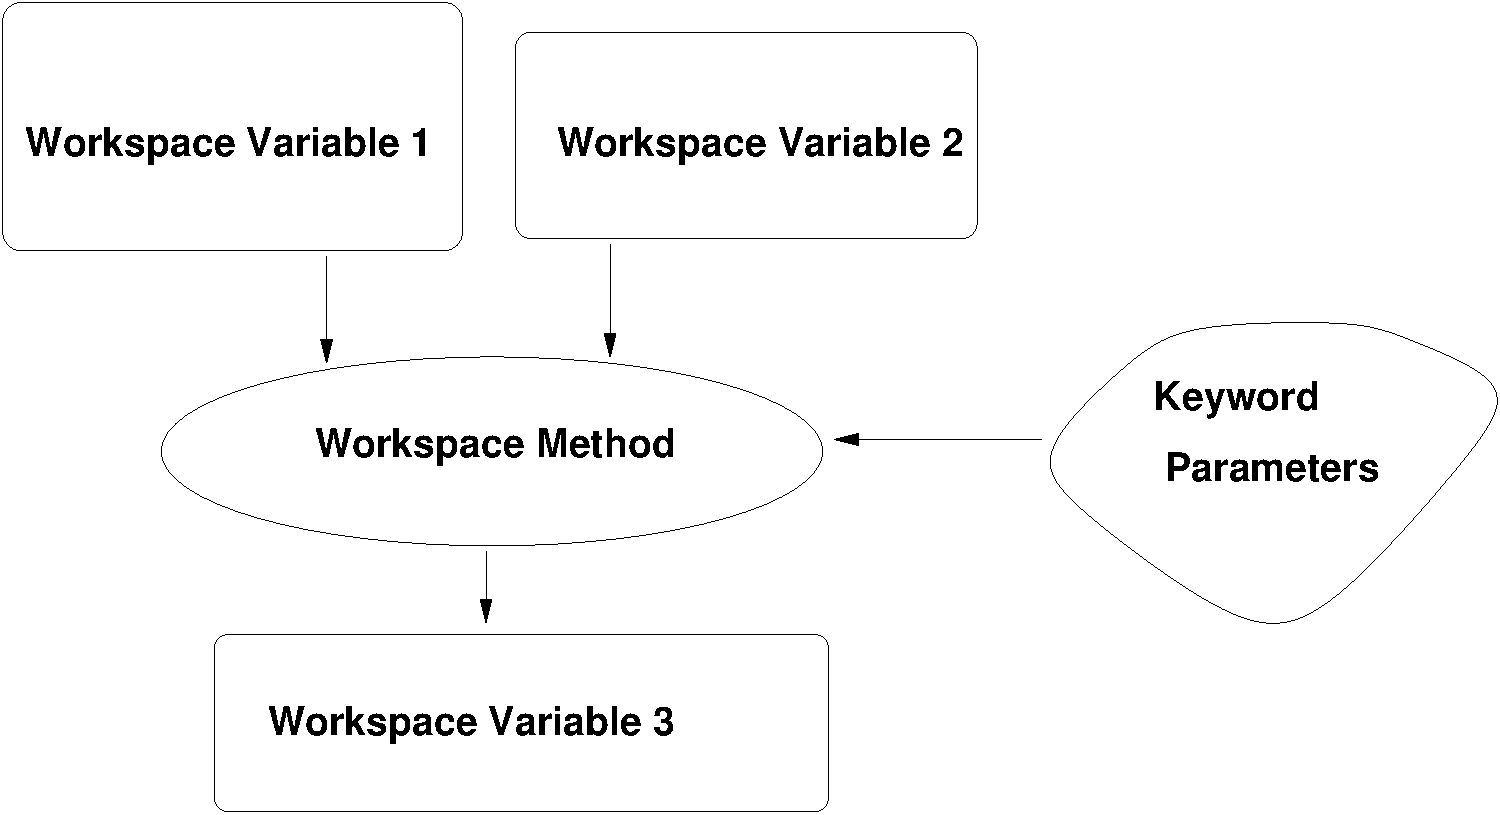
\includegraphics[width=\hsize,draft=false]{concept/method}
    \caption{\textindex{Specific
        workspace methods} act on specific workspace variables to
        generate other specific workspace variables. Additional input
        parameters can be specified as keyword parameters in the
        controlfile.}
    \label{fig:method}
  \end{center}
\end{figure}

It is important to note that the controlfile has a fixed and
well-defined syntax. This syntax is understood by the ARTS parser.
The great advantage of this concept is that it is very easy to add
new workspace variables and new workspace methods. The program has
an internal lookup table which lists all workspace methods, as well
as their input variables, output variables, and keyword
parameters. To add a new method, one just has to add an entry to
this lookup table, and write the code for the method itself. No
further changes to the program are necessary. In particular, no
changes to the program logic or to the parser. How such an extension
can be made practically is described in Section \ref{sec:development}.


\section{Generic Workspace Methods}
%=================================
\label{sec:concept:generic}

Generic methods (Figure \ref{fig:generic_method}) allow the user of
the program even more freedom than specific methods. A generic method
is for example \artsstyle{MatrixSet}, which can be used to set any
workspace variable which is a matrix. For example
\begin{quote}
  \artsstyle{MatrixSet(z\_surface){0.0}}
\end{quote}
will set all elements of \artsstyle{z\_surface} to 0.0 (as long as
\artsstyle{nrows} and \artsstyle{ncols} are set).

\begin{figure}
  \begin{center}
    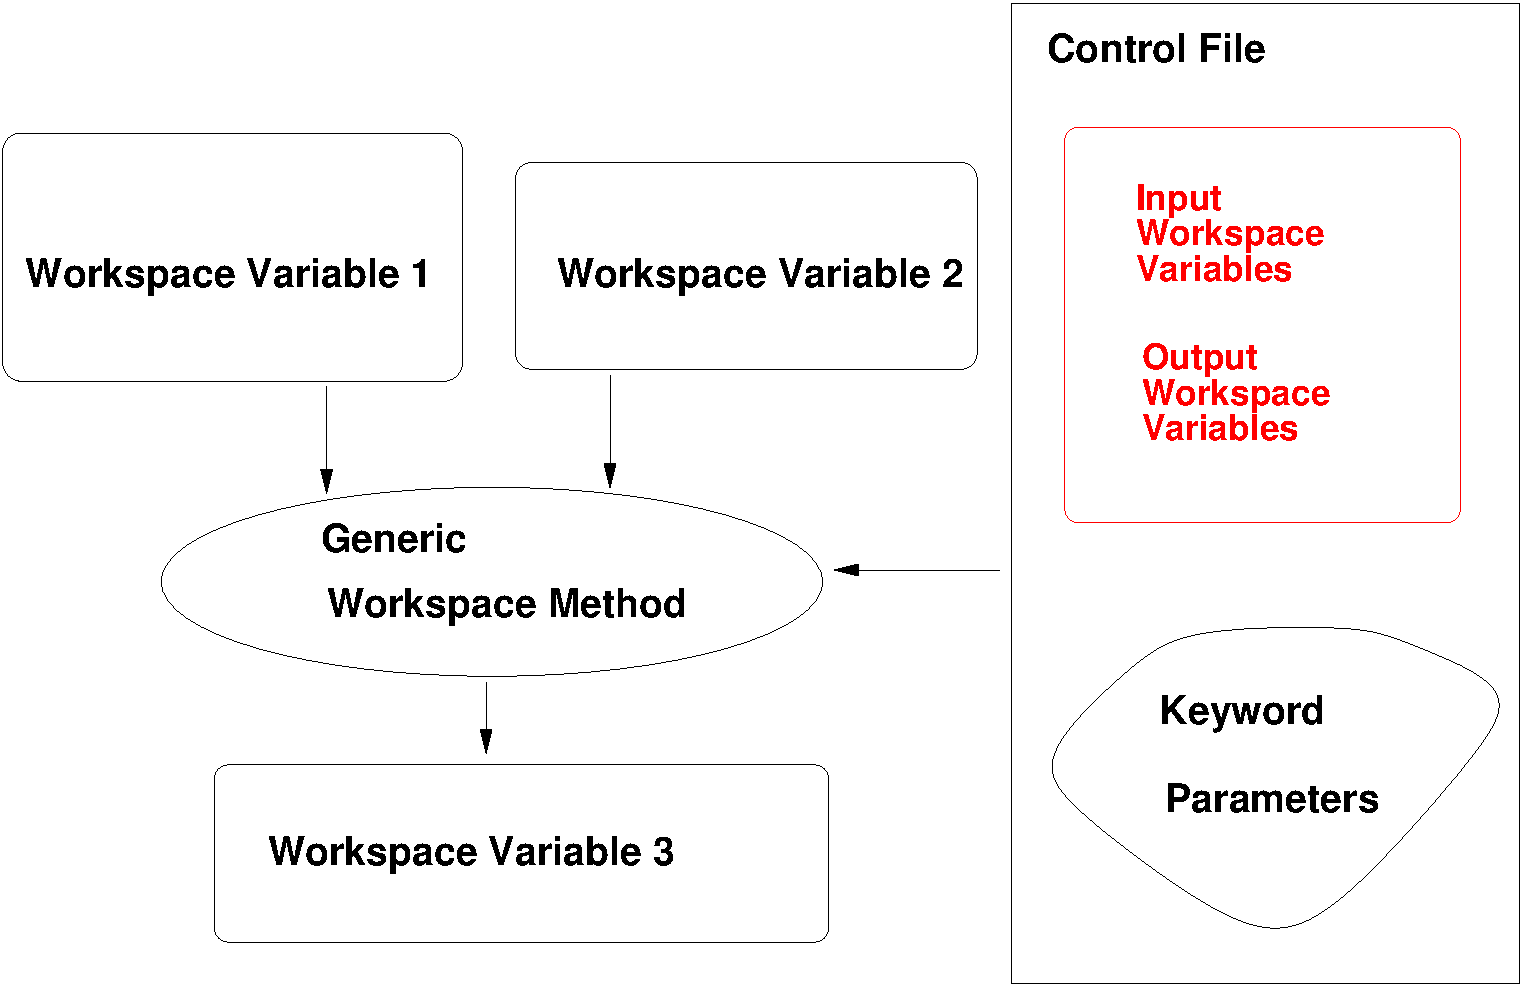
\includegraphics[width=\hsize,draft=false]{concept/generic_method}
    \caption{For \textindex{generic
      workspace methods} the workspace variables to act on are
        specified in the controlfile.}
    \label{fig:generic_method}
  \end{center}
\end{figure}

Some methods are even more flexible, the are super generic. This means
that they can take any workspace variable as input. The most commonly
used such methods are the XML file methods. A workspace variable is
read from a file in this way
\begin{quote}
  \artsstyle{ReadXML(f\_grid)\{"frequency\_grid"\}}
\end{quote}
Generic methods are particularly useful for IO operations like in the
example above. No new IO methods are necessary for new workspace
variables, as long as they are of standard types already known to the
program (for example vectors or matrices). 



\section{Agendas}
%=================================
\label{sec:concept:agendas}

Agendas are a special incarnation of a workspace method. In the
controlfile an arbitrary number of workspace methods can be added to
an agenda. On invocation, the agenda executes its methods one
after the other. The inputs and outputs defined for the agenda must
be satisfied by the invoked workspace methods. E.g., if an agenda
has \artsstyle{f\_grid} in its list of output workspace variables, a
workspace method which generates \artsstyle{f\_grid} must be added to
the agenda in the controlfile.

Even though it is possible to execute agendas directly from the
controlfile with the \artsstyle{AgendaExecute} method, the more common
and intended use case is the internal invocation by other workspace
methods. This adds a grave amount of flexibility to arts. The
\artsstyle{RteStd} method for example calculates (besides other
components) the emission term. Without the means of an agenda, it
would only be possible to use always the same method for the emission
calculation. By the use of an agenda the user can choose between
different methods to calculate the emission and plug them into the
emission agenda in the control file:

{\small
\begin{verbatim}
AgendaSet(emission_agenda){
  emissionPlanck{}
}
\end{verbatim}
}

\noindent
\artsstyle{RteStd} internally calls the \artsstyle{emission\_agenda} and
uses the user selected method for calculating the emission term.



\section{Practical hints}
%=================================
\label{sec:concept:practical}

The subdirectory \fileindex{tests} contains some example controlfiles.
You should study them to learn more about how the program works. You
can also run these controlfiles like this:
\begin{quote}
\begin{verbatim}
  arts TestAbs.arts
\end{verbatim}
\end{quote}
This assumes that you are inside the directory where the controlfiles
are, and that the \artsstyle{arts} executable is in your path.  You can
also run all of the examples, by saying
\begin{quote}
\begin{verbatim}
  make check
\end{verbatim}
\end{quote}

ARTS offers a number of useful command line parameters. In general,
there is a short form and a long form for each parameter. The short
form consists of a minus sign and a single letter, whereas the long
form consists of two minus signs and a descriptive name. To get a full
list, type
\begin{quote}
\begin{verbatim}
  arts -h
\end{verbatim}
\end{quote}
or
\begin{quote}
\begin{verbatim}
  arts --help
\end{verbatim}
\end{quote}
Most useful at the beginning should be the \artsstyle{-d}
(\artsstyle{--describe}), \artsstyle{-m} (\artsstyle{--methods}), \artsstyle{-w}
(\artsstyle{--workspacevariables}), and \artsstyle{-i} (\artsstyle{--input}) flags.
For instance, the \artsstyle{-d} (\artsstyle{--describe}) flag gives you online
documentation for any workspace method or workspace variable. Usage:
\begin{quote}
\begin{verbatim}
  arts -d f_grid
\end{verbatim}
\end{quote}
will print documentation about the workspace variable \artsstyle{f\_grid}, which
happens to be the monochromatic frequency grid.

But what methods and variables are available? You can find out by
typing
\begin{quote}
\begin{verbatim}
  arts -m all
\end{verbatim}
\end{quote}
which will list all workspace methods, or by typing 
\begin{quote}
\begin{verbatim}
  arts -w all
\end{verbatim}
\end{quote}
which will list all workspace variables. As you can see, these lists
are quite long. But you can get more specific information:
\begin{quote}
\begin{verbatim}
  arts -m f_grid
\end{verbatim}
\end{quote}
will give you a list of all methods that can generate the workspace
variable \artsstyle{f\_grid}. Specific and generic methods are listed
separately. Generic methods are in this case all methods producing a
Vector, since \artsstyle{f\_grid} belongs to this group. A similar task is
performed by the \artsstyle{-i} (\artsstyle{--input}) flag, with the difference
that \artsstyle{arts -i f\_grid} will list those methods that require
\artsstyle{f\_grid} as \emph{input}, whereas \artsstyle{arts -m f\_grid} lists
those that produce \artsstyle{f\_grid} as output. Finally,
\begin{quote}
\begin{verbatim}
  arts -w surfaceFlat
\end{verbatim}
\end{quote}
will give you all variables required by the method \artsstyle{abs\_coefCalc}
(the variable \artsstyle{f\_grid} happens to be one of them).

Using these command line parameters, it is easy to build up a
controlfile. The trick is, to start at the end. Say you want to
compute absorption coefficients. First of all, you have to find out
in which workspace variable these are stored. Look at the list
produced by \artsstyle{arts -w all}. You can use \artsstyle{arts -d} to look at
some candidates a bit more closely. This way, you will find out that
\artsstyle{abs\_coef} is the variable you are looking for.

In the next step, you can use \artsstyle{arts -m abs\_coef} to find all methods
that can calculate \artsstyle{abs\_coef}. So, you will find the method
\artsstyle{abs\_coefCalc}. Now you can use \artsstyle{arts -w abs\_coefCalc} to find out the
required input variables of that method. Then you can use the
\artsstyle{-m} flag again, to find the methods producing these variables,
and so on.

%%% Local Variables: 
%%% mode: latex
%%% TeX-master: "uguide"
%%% End: 

\chapter{Importing and exporting data}
 \label{sec:inout}


 \starthistory
 ? & ?.\\
 \stophistory

Sorry, so far just a few words about supported data formats.\\ \\

\FIXME{Extend this chapter.}


\section{Data formats}

\subsection{XML files}

% FIXME: OLE: Extend this
XML is the default file format for exchanging data with ARTS. Two flavors are
supported: Plain text and binary. In the plain format all data is stored in
the XML file. For binary, the structure of the data is stored in the XML file
and the data itself in binary format in a separate file.

\subsection{NetCDF files}

% FIXME: OLE: Extend this
NetCDF input and output is supported for a subset of the data types available
in ARTS.

\subsection{Gridded fields}

\subsubsection{Naming convention for grids}

% FIXME: OLE: Extend this
\begin{alltt}
\small
\input{gridded_field_gridnames.txt}
\end{alltt}



%%% Local Variables: 
%%% mode: latex
%%% TeX-master: "main"
%%% End: 

\chapter{Description of the atmosphere}
 \label{sec:atmosphere}

\starthistory
 120831 & Revised by Patrick Eriksson.\\ 
 020315 & First version by Patrick Eriksson.\\
\stophistory

\graphicspath{{Figs/atmosphere/}}

This section discusses the model atmosphere: how it is defined, its boundaries
and the variables describing the basic properties. One aspect that can cause
confusion is that several vertical coordinates must be used
(Section~\ref{sec:fm_defs:altitudes}). The main vertical coordinate is pressure
and atmospheric quantities are defined as a function of pressure
(Section~\ref{sec:fm_defs:grids}), but the effective vertical coordinate from a
geometrical perspective (such as the determination of propagation paths) is the
radius (Section~\ref{sec:fm_defs:atmdim}). Pressures and radii are linked by
specifying the geometrical altitudes (\builtindoc{z\_field}).


\section{Altitude coordinates}
%===================
\label{sec:fm_defs:altitudes}

\begin{description}
  
\item[Pressure\index{pressure}] The main altitude coordinate is
  pressure. This is most clearly manifested by the fact that the
  vertical atmospheric grid consists of equal-pressure levels.
  The vertical grid is consistently denoted as the pressure grid and
  the corresponding workspace variable is \wsvindex{p\_grid}. The
  choice of having pressure as main altitude coordinate results in
  that atmospheric quantities are retrieved as a function of pressure,
  not as a function of geometrical altitude.
  
\item[Pressure altitude\index{pressure altitude}] A basic assumption
  in ARTS is that atmospheric quantities (temperature, geometric
  altitude, species VMR etc.) vary linearly with the logarithm of the
  pressure. This corresponds roughly to assuming a linear variation
  with altitude. 

\item[Radius\index{radius}] Geometrical altitudes are
  needed to determine the propagation path through the atmosphere etc.
  The main geometrical altitude coordinate is the distance to the
  centre of the coordinate system used, the radius. This is a natural
  consequence of using a spherical or polar coordinate system. The
  radius is used inside ARTS for all geometrical calculations.
  
\item[Geometrical altitude\index{geometrical altitude}] The term geometrical
  altitude signifies here the difference in radius between a point and the
  reference ellipsoid (Section \ref{sec:fm_defs:geoid}) along the vector to the
  centre of the coordinate system (Equation \ref{eq:fm_defs:zsurface}). This is
  consistent with the usage of geocentric latitudes (see below). Hence, the
  altitude is not measured along the local zenith direction.
\end{description}



\section{Atmospheric dimensionality}
%===================
\label{sec:fm_defs:atmdim}

The structure of the modelled atmosphere can be selected to have different
degree of complexity, the \textindex{atmospheric dimensionality}. There exist
three options, 1D, 2D and 3D, where 1D and 2D can be seen as special cases of
3D. The significance of these different atmospheric dimensionalities and the
geometrical coordinate systems used are described below in this section. The
atmospheric dimensionality is selected by setting the workspace variable
\wsvindex{atmosphere\_dim} to a value between 1 and 3. The atmospheric
dimensionality is most easily set by the functions \wsmindex{AtmosphereSet1D},
\wsmindex{AtmosphereSet2D} and \wsmindex{AtmosphereSet3D}.

\begin{figure}
 \begin{center}
  \includegraphics*[width=0.98\hsize]{atm_dim_1d}
  \caption{Schematic of a 1D atmosphere. The atmosphere is 
    here spherically symmetric. This means that the radius of the
    ellipsoid, the surface and all the pressure levels are constant
    around the globe. The fields are specified by a value for each
    pressure level. The extension of the cloud box is either from
    the surface up to a pressure level, or between two pressure
    levels (which is the case shown in the figure). The figure indicates
    also that the surface must be above the lowermost pressure
    level. (``Geoid'' in the legend should be ``Ellipsoid''.)}
  \label{fig:fm_defs:1d}  
 \end{center}
\end{figure}
% This figure was produced by the Matlab function mkfigs_atm_dims.

\begin{figure}
 \begin{center}
  \includegraphics*[width=0.98\hsize]{atm_dim_2d}
  \caption{Schematic of a 2D atmosphere. The radii (for the surface
    and the pressure levels) vary here linear between the latitude
    grid points. The atmospheric fields vary linearly along the
    pressure levels and the latitude grid points (that is, along the
    dotted lines). Inside the grid cells, the fields have a bi-linear
    variation. No cloud box is included in this figure.
    (``Geoid'' in the legend should be ``Ellipsoid''.)}
  \label{fig:fm_defs:2d}
 \end{center}
\end{figure}
% This figure was produced by the Matlab function mkfigs_atm_dims.

\begin{description}
  
\item[\textindex{1D}\,\,\,] A 1D atmosphere can be described as being
  spherically symmetric. The term 1D is used here for simplicity and historical
  reasons, not because it is a true 1D case (a strictly 1D atmosphere would
  just extend along a line). A spherical symmetry means that atmospheric fields
  and the surface extend in all three dimensions, but they have no latitude and
  longitude variation. This means that, for example, atmospheric fields vary
  only as a function of altitude and the surface constitutes the surface of a
  sphere. The radial coordinate is accordingly sufficient when dealing with
  atmospheric quantities. The latitude and longitude of the sensor are normally
  of no concern, but when required the sensor is considered to be placed at
  latitude and longitude zero $([\Lat,\Lon]=[0,0])$. The sensor is assumed to
  by directed towards the North pole, corresponding to an azimuth angle of
  0\degree. A 1D atmosphere is shown in Figure~\ref{fig:fm_defs:1d}.
  
\item[\textindex{2D}\,\,\,] In contrast to the 1D and 3D cases, a 2D atmosphere
  is only strictly defined inside a plane. More in detail, this case be seen as
  observations restricted to the plane where the longitude equals 0\degree\ or
  180\degree. A polar system\index{polar coordinate system}, consisting of a
  radial and an angular coordinate, is applied. The angular coordinate is
  denoted as latitude, and matches the 3D latitude in the range
  $[-90\degree,+90\degree]$, but for 2D there is no lower or upper limit for
  the latitude coordinate. The 2D case is most likely used for satellite
  measurements where the atmosphere is observed inside the orbit plane. The 2D
  ``latitude'' can then be taken as the angular distance along the satellite
  track. A 2D-latitude of e.g.\ 100\degree\ will then correspond to a
  2D-latitude of 80\degree. The atmosphere is normally treated to be undefined
  outside the considered plane, but some scattering calculations may treat the
  surrounding atmosphere in an simplified manner. A 2D atmosphere is shown in
  Figure~\ref{fig:fm_defs:2d}.

\item[\textindex{3D}\,\,\,] In this, the most general, case, the atmospheric
  fields vary in all three spatial coordinates, as in a true atmosphere
  (Figures~\ref{fig:fm_defs:3d}). A
  \textindex{spherical coordinate system} is used where the dimensions are
  radius (\Rds), latitude (\Lat) and longitude (\Lon), and a position is given
  as $(\Rds,\Lat,\Lon)$. With other words, the standard way to specify a
  geographical position is followed. The valid range for latitudes is
  $[-90\degree,+90\degree]$, where +90\degree corresponds to the North pole
  etc. Longitudes are counted from the Greenwich meridian with positive values
  towards the east. Longitudes can have values from -360\degree to +360\degree.
  When the difference between the last and first value of the longitude grid is
  $360\degree$ then the whole globe is considered to be covered. The user
  must ensure that the atmospheric fields for \Lon\ and $\Lon+360\degree$ are
  equal. If a point of propagation path is found to be outside the range of the
  longitude grid, this will results in an error if not the whole globe is
  covered. When possible, the longitude is shifted with 360\degree\ in the
  relevant direction.
  

\end{description}

\begin{figure}[t]
 \begin{center}
  \includegraphics*[angle=-90,width=0.98\hsize]{atm_dim_3d}
  \vspace*{-15mm}
  \caption{Schematic of a 3D atmosphere. Plotting symbols as in 
    Figure \ref{fig:fm_defs:2d}. Radii and fields are here defined to
    vary linearly along the latitude and longitude grid points. This
    means that the radius of a pressure level has a
    bi-linear variation inside the area limited by two latitude and
    longitude grid values, while the atmospheric fields have a
    tri-linear variation inside the grid cells. }
  \label{fig:fm_defs:3d}
 \end{center}
\end{figure}
% This figure was produced by the Matlab function mkfigs_atm_dims.

% \begin{figure}[p]
%  \begin{center}
%   \includegraphics*[width=0.98\hsize]{atm_dim_3dcross}
%   \caption{A latitudinal, or longitudinal, cross section of a 3D atmosphere. 
%     Plotting symbols as in Figure \ref{fig:fm_defs:1d}. Radii and
%     fields inside the cross section match the definitions for 2D.
%     The vertical extension
%     of the cloud box is defined identical for 1D and 3D. The horizontal 
%     extension of the cloud box is between two latitude and longitude grid
%     positions, where only one of the dimensions is visible in this figure.}
%   \label{fig:fm_defs:3dcross}
%  \end{center}
% \end{figure}
% % This figure was produced by the Matlab function mkfigs_atm_dims.



\section{Atmospheric grids and fields}
%===================
\label{sec:fm_defs:grids}

As mentioned above, the vertical grid of the atmosphere consists of a
set of layers with equal pressure, the pressure grid
(\wsvindex{p\_grid}).  This grid must of course always be specified.
The upper end of the pressure grid gives the practical upper limit of
the atmosphere as vacuum is assumed above. With other words, no
absorption and refraction take place above the uppermost pressure
level.

A \textindex{latitude} grid (\wsvindex{lat\_grid}) must be specified for 2D and
3D. For 2D, the latitudes shall be treated as the angular distance along the
orbit track, as described above in Section \ref{sec:fm_defs:atmdim}. The
latitude angle is throughout calculated for the vector going from the centre of
the coordinate system to the point of concern. Hence, the latitudes here
correspond to the definition of the geocentric latitude, and not geodetic
latitudes (see Section \ref{sec:ppath:geoid}). This is in accordance to the
definition of geometric altitudes (Section~\ref{sec:fm_defs:altitudes}). For
3D, a \textindex{longitude} grid (\wsvindex{lon\_grid}) must also be specified.
Valid ranges for latitude and longitude values are given in Section
\ref{sec:fm_defs:atmdim}. If the longitude and latitude grids are not used for
the selected atmospheric dimensionality, then the longitude grid (for 1D and
2D) and the latitude grid (for 1D) must be set to be empty.


The atmosphere is treated to be undefined outside the latitude and longitude
ranges covered by the grids, if not the whole globe is covered. This results in
that a propagation path is not allowed to cross a latitude or longitude end
face of the atmosphere, if such exists, it can only enter or leave the
atmosphere through the top of the atmosphere (the uppermost pressure level).
See further Section \ref{sec:fm_defs:ppaths}. The volume covered by the grids
is denoted as the \textindex{model atmosphere}.

The basic atmospheric quantities are represented by their values at each
crossing of the involved grids (indicated by thick dots in Figure
\ref{fig:fm_defs:2d}), or for 1D at each pressure
level (thick dots in Figure \ref{fig:fm_defs:1d}). This representation is
denoted as the field\index{atmospheric field} of the quantity. The field must,
at least, be specified for the geometric altitude of the pressure levels
(\wsvindex{z\_field}), the temperature (\wsvindex{t\_field}) and considered
atmospheric species (\builtindoc{vmr\_field}). The fields are assumed to be
piece-wise linear functions vertically (with pressure altitude as the vertical
coordinate, Section \ref{sec:fm_defs:altitudes}), and along the latitude and
longitude edges of 2D and 3D grid boxes. For points inside 2D and 3D grid
boxes, multidimensional linear interpolation is applied (that is, bi-linear
interpolation for 2D etc.). Note especially that this is also valid for the
field of geometrical altitudes (\builtindoc{z\_field}). Fields are rank-3
tensors. For example, the temperature field is $T=T(\Prs,\Lat,\Lon)$. That
means each field is like a book, with one page for each pressure grid point,
one row for each latitude grid point, and one column for each longitude grid
point. In the 1D case there is just one row and one column on each page. The
representation of atmospheric fields, and other quantities, is discussed
further in Section~\ref{sec:wfuns:basis}, where the concept of basis
functions\index{basis function} is introduced. In short, the basis functions
give the mapping from the set of discrete values to the continuous
representation of the quantity.



\section{Geo-location of 1D and 2D}
%===================
\label{sec:fm_defs:geoloc}

For 1D and 2D atmospheres, \builtindoc{lat\_grid} and \builtindoc{lon\_grid} do
not contain true geographical positions (they are either empty or
\builtindoc{lat\_grid} contains transformed data). However, some operations
require that the positions is known, and this \index{geo-location} is handled
by \wsvindex{lat\_true} and \wsvindex{lon\_true}. See the built-in
documentation for further information on how to specify these variables.



\section{Hydrostatic equilibrium}
%===================
\label{sec:fm_defs:hse}

There is no general demand that the model atmosphere fulfils hydrostatic
equilibrium. That is, \builtindoc{t\_field} and \builtindoc{z\_field} can be
specified independently of each other. On the other hand, ARTS provides means
for ensuring that a model atmosphere matches hydrostatic equilibrium by the
method \wsmindex{z\_fieldFromHSE}. The method considers that gravitation varies
with latitude and altitude, and \builtindoc{lat\_true} and
\builtindoc{lon\_true} must be set for 1D and 2D.

Hydrostatic equilibrium gives only constrain for the distance between the
pressure levels, not for the absolute geometrical altitudes. For this reason, a
``reference point'' must be introduced. This is done by setting the pressure of
this point by \wsvindex{p\_hse} (common for all latitude and longitudes). The
geometrical altitudes matching \builtindoc{p\_hse} are taken from the original
values in \wsvindex{z\_field}. 


\section{The reference ellipsoid and the surface}
%===================
\label{sec:fm_defs:surf}

Geometrical altitudes are specified as the vertical distance to the reference
ellipsoid (\wsvindex{refellipsoid}), discussed further in Section
\ref{sec:fm_defs:geoid}. The lower boundary of the atmosphere is denoted as the
surface. The surface is specified by its geometrical altitude on the latitude
and longitude grids. The workspace variable holding these data is called
\wsvindex{z\_surface}.

It is not allowed that there is an altitude gap between the surface and
the lowermost pressure level.  That is, the surface pressure must be
smaller than the pressure of the lowermost vertical grid level. On
the other hand, it is not necessary to match the surface and the first
pressure level, the pressure grid can extend below the surface level.


\section{The cloud box}
%===================
\label{sec:fm_defs:cloudbox}
In order to save computational time, calculations involving scattering are
limited to a special atmospheric domain. This atmospheric region is denoted as
the \textindex{cloud box}. The cloud box is discussed here as it acts as an
additional atmospheric limit when calculating propagation paths (see Section
\ref{sec:fm_defs:rte}).

The cloud box is defined to be rectangular in the used coordinate
system, with limits exactly at points of the involved grids. This
means, for example, that the vertical limits of the cloud box are two
pressure levels. For 3D, the horizontal extension of the cloud box
is between two points of the latitude grid and likewise in the
longitude direction. The latitude
and longitude limits for the cloud box cannot be placed at the end
points of the corresponding grid as it must be possible to calculate
the incoming intensity field. The cloud box is activated by setting
the variable \wsvindex{cloudbox\_on} to 1.  The limits of the cloud
box are stored in \wsvindex{cloudbox\_limits}.  It is recommended to
use the method \wsmindex{CloudboxOff} when no scattering calculations
shall be performed. This method assigns dummy values to all workspace
variables not needed when scattering is neglected.

When the radiation entering the cloud box is calculated this is done
with the cloud box turned off. This to avoid to end up in the
situation that the radiation entering the cloud box depends on the
radiation coming out from the cloud box. {\bf It is the task of the
  user to define the cloud box in such way that the link between the
  outgoing and ingoing radiation fields of the cloud box can be
  neglected}. The main point to consider here is radiation reflected
by the surface. To be formally correct there should never be a gap
between the surface and the cloud box. This is the case as radiation
leaving the cloud box can then be reflected back into the cloud box by
the surface. If it is considered that the surface is a scattering object
it is clear that the surface should in general be part of the cloud
box. However, for many cases it can be accepted to have a gap between
the surface and the cloud box, with the gain that the cloud box can be
made smaller. Such a case is when the surface is treated to act as
blackbody, the surface is then not reflecting any radiation.
Reflections from the surface can also be neglected if the zenith
optical thickness of the atmosphere between the surface and cloud box
is sufficiently high.


%%% Local Variables: 
%%% mode: latex
%%% TeX-master: "uguide"
%%% End: 

\chapter{Radiative transfer basics}
 \label{sec:rte_basics}

\starthistory
 130218 & First version by Patrick Eriksson.\\
\stophistory

This chapter introduces some basic radiative transfer nomenclature and
equations. The radiative transfer equation is here presented in general terms,
while special cases and solutions are discussed in later parts of the document.



\section{Stokes dimensionality}
%==============================================================================
\label{sec:fm_defs:polarisation}

The full polarisation state of radiation can be described by the Stokes vector,
and is the formalism applied in ARTS. The vector can be defined in different
ways, but it has always four elements. The Stokes vector, \StoVec, is here
written as
\begin{equation}
  \label{eq:fm_defs:stokevec}
  \StoVec = \left[
  \begin{array}{c}
   \StoI\\ \StoQ \\ \StoU\\ \StoV
  \end{array}
  \right],
\end{equation}
where the first component (\StoI) is the full intensity of the
radiation, the second component (\StoQ) is the difference between
vertical and horizontal polarisation, the third component (\StoU) is the
difference for $\pm$45$^\circ$ polarisation and the last component
(\StoV) is the difference between left and right circular polarisation.
That is:
\begin{eqnarray}
  \StoI &=&   \Iv + \Ih = \Ipff + \Imff = \Ilhc + \Irhc, \\
  \StoQ &=&   \Iv - \Ih,                                 \\
  \StoU &=&   \Ipff - \Imff,                             \\
  \StoV &=&   \Ilhc - \Irhc,                             
\end{eqnarray}
where \Iv, \Ih, \Ipff, and \Imff\ are the intensity of the component linearly
polarised at the vertical, horizontal, +45\degree\ and -45\degree\ direction,
respectively, and \Irhc, and \Ilhc\ are the intensity for the right- and
left-hand circular components. Further details on polarisation and the
definition of the Stokes vector are found in \theory,
Section~\ref{T-sec:polarization}.

ARTS is a fully polarised forward model, but can be run with a smaller number
of Stokes components. The selection is made with the workspace variable
\wsvindex{stokes\_dim}. For example, gaseous absorption and emission are in
general unpolarised, and if not particle and surface scattering have to be
considered it is sufficient to only include the first Stokes components in the
simulations (ie.\ \builtindoc{stokes\_dim} set to 1). In this case, to include
higher order Stokes components results only in slower calculations. Simulations
where \builtindoc{stokes\_dim} is two or higher are denoted as
\textindex{vector radiative transfer}, while \textindex{scalar radiative
  transfer} refers to the case when only the first Stokes component is
considered.
 



\section{The radiative transfer equation}
%==============================================================================
\label{sec:rteq}

The radiative transfer problem can only be expressed in a general manner as a
differential equation. One version for vector radiative transfer is
\begin{equation}
  \label{eq:VRTE0}
  \frac {\DiffD\StoVec(\Frq,\PPos,\PDir)}{\DiffD \PpathLng} =
    -\ExtMat(\Frq,\PPos,\PDir) \StoVec(\Frq,\PPos,\PDir) +
    \aSrcVec{e}(\Frq,\PPos,\PDir) + \aSrcVec{s}(\Frq,\PPos,\PDir),  
\end{equation}
where \Frq\ is frequency, \PPos\ represents the atmospheric position, \PDir\ is
the propagation direction (at \PPos), \PpathLng\ is distance along \PDir,
\ExtMat\ is the propagation matrix, \aSrcVec{e}\ represents the emission at
the point, and \aSrcVec{s}\ covers the scattering from other directions into
the propagation direction.



\subsection{Propagation effects}
\label{sec:rteq:propmat}

Three mechanisms contribute to the elements of the propagation matrix:
absorption, scattering and magneto-optical effects. Absorption and scattering
can together be denoted as extinction, referring to that these two mechanisms
result in a decrease of the intensity (\StoI). A common name for \ExtMat\ is
also the extinction matrix. The extinction processes also affect the \StoQ,
\StoU\ and \StoV\ elements of the Stokes vector. If the degree of polarisation
(\DgrPlr)
\begin{equation}
  \label{eq:degreeofpol}
  \DgrPlr = \frac{\sqrt{\StoQ^2+\StoU^2+\StoV^2}}{\StoI}
\end{equation}
is kept constant or not depend on symmetry properties of the attenuating media.
For example, absorption of atmospheric gases is not changing \DgrPlr\ as long
as the molecules have no preferred orientation, which is a valid assumption
beside when there is a significant Zeeman effect. Non-polarising absorption
corresponds to that the propgation matrix can be written as $\AbsCoef\IdnMtr$,
where \AbsCoef\ is the absorption coefficient and \IdnMtr\ is the identity
matrix.

There are also examples on effects that change the polarisation state of the
Stokes vector without affecting \StoI. These effects are caused by an
interaction with the magnetic field, and are thus denoted magneto-optical.
Ionospheric Faraday rotation can (approximately) be seen as a pure
magneto-optical effect, while the Zeeman effect cause both non-isotropic
absorption and has magneto-optical aspects.

As Equation~\ref{eq:VRTE0} indicates, there are two source mechanisms that can
act to increase the intensity: emission and scattering.


\subsection{Absorbing species and scattering particles}
\label{sec:rteq:absspecies}

The complexity of the radiative transfer is largely dependent on whether scattering
must be considered or not. For this reason, ARTS operates with two classes of
atmospheric matter:
\begin{description}
\item[Absorbing species] This class covers atmospheric matter for which
  scattering can be neglected. The set of ``species'' to consider is described
  by the workspace variable \wsvindex{abs\_species}, and the associated
  atmospheric fields are gathered into \wsvindex{vmr\_field}. As the name
  indicates, this later variable is mainly containing volume mixing ratio (VMR)
  data, but as this unit is not applicable in all cases also other units are
  accepted. That is, the unit for the fields varies, for gases it is VMR, while
  particle mass concentrations are given in $kg/m^3$ and electron density in
  $m^{-3}$. 
\item[Particles] This second class treats all matter causing significant
  scattering (and likely also adding to the absorption). The amount of
  scattering matter is given as particle number density fields ($m^{-3}$),
  denoted as \wsvindex{pnd\_field}. The \wsvindex{pnd\_field} is provided per
  scattering element (see Chapter \ref{sec:clouds} for definition). The
  corresponding optical properties of the particles are given by
  \wsvindex{scat\_data} containing one set of single scattering properties
  for each scattering element. Particles can be grouped into scattering
  species, each characterized by a mass density ($kg/m^3$) or flux ($kg/(m^2s$)
  field that is converted into particle number density fields before solving the
  radiative transfer equation.
\end{description}
Atmospheric quantities are not hard-coded to belong to any of these matter
classes, as the practical division depends on the conditions of the
simulations. The general rule is that for the shorter the wavelengths, a higher
number of atmospheric constituents must be treated as ``particles''. For
thermal infrared and microwave calculations, molecules and electrons (and
likely also aerosols) can be treated as absorbing species. It can also be
possible to place some hydrometeors in this class. For example,
non-precipitating liquid clouds can be treated as purely absorbing in the
microwave region.
Related to the division between absorbing species and particles is:
\begin{description}
\item[Clear-sky] In ARTS, the term ``clear-sky'' refers to the case when the
  influence of ``particles'' can be ignored, and only ``absorbing species'' are
  of relevance. Hence, a clear-sky calculation can involve e.g.\ cloud water
  droplets, but on the condition that the wavelength is such that scattering
  can be neglected.
\end{description}
The propagation effects of absorbing species and of (scattering) particles are
kept separated.
The total propagation matrix is 
\begin{equation}
  \label{eq:propmattotal}
  \ExtMat = \aAbsMat{a} + \aExtMat{p}, 
\end{equation}
where $a$ and $p$ refers to absorbing species and particles, respectively, and
the symbol \AbsMat\ is used for the first term to remind about that the only
extinction process covered by this matrix is absorption (but including
magneto-optical effects). As workspace variable, \aAbsMat{a}\ is denoted as
\wsvindex{propmat\_clearsky}, obtained by the
\wsaindex{propmat\_clearsky\_agenda} agenda. \aExtMat{p}\ is obtained
internally from \builtindoc{scat\_data}.



\subsection{Emission and absorption vectors}
\label{sec:rteq:evec}

One of the general assumptions in ARTS is that local thermodynamic equilibrium
(LTE) can be assumed. For the moment there exists no method in ARTS to handle
deviations from LTE, but this can be changed in the future.
On the condition of LTE, the emission vector ($\VctStl{j}_e$) in
Equation~\ref{eq:VRTE0} can be written as
\begin{equation}
  \label{eq:evec1}
  \aSrcVec{e} = \Planck \AbsVec,
\end{equation}
where \Planck\ is the Planck function (a scalar value), describing blackbody
radiation. For non-LTE, the emission vector
is instead
\begin{equation}
  \label{eq:evec_withnlte1}
  \aSrcVec{e} = \Planck\aAbsVec{s},
\end{equation}
where the source term \aAbsVec{s}\ contains both LTE and non-LTE effects.
We code non-LTE not as above but with the concept of ``relative additional'' non-LTE effects.  
This additional non-LTE effect is named \wsvindex{nlte\_source} and it has the form
\begin{equation}
  \label{eq:nlte_source}
  \aSrcVec{n} = \Planck\left(\aAbsVec{s}\oslash\AbsVec-1\right).
\end{equation}
(Note that the operator means that we are using element-wise division.  Below, the dot means element-wise multiplication.)
The idea here is that \aSrcVec{e} in Equation~\ref{eq:evec2} is never directly used
but instead
\begin{equation}
  \label{eq:evec_withnlte2}
  \aSrcVec{e} = \AbsVec\odot\left(\Planck + \aSrcVec{n}\right).
\end{equation}

The quantity \AbsVec\ is denoted as the absorption vector. For clear-sky
calculations the absorption vector is given by \aAbsMat{a}, as in this case the
emission vector can be calculated as
\begin{equation}
  \label{eq:evec2}
  \aSrcVec{e} = \aAbsMat{a}\EmsVec,
\end{equation}
where \EmsVec\ can be seen as the emission source vector, defined as
\begin{equation}
  \EmsVec = [\Planck,0,0,0]^T.
\end{equation}
Hence, as only the first element of \EmsVec\ is non-zero, the absorption
vector is in this case equal to the first column of \aAbsMat{a}.
The absorption vector can not be extracted from \aExtMat{p}\ as this
propagation matrix covers also scattering and \wsvindex{scat\_data}
must also contain such data.

In summary, the total absorption vector in ARTS is obtained as
\begin{equation}
  \label{eq:evec3}
  \AbsVec = \aAbsVec{a} + \aAbsVec{p}
\end{equation}
where \aAbsVec{a}\ is the first column of \aAbsMat{a}\, and \aAbsVec{p}\ is the
absorption vector due to particles.




\subsection{Main cases}
\label{sec:rteq:cases}
%
The two equations below are discussed thoroughly in \ref{T-sec:rte_theory} of
\theory. This including that for some conditions also the ``n2-law of
radiance'' must be considered to obtain completely exact results (see also
Section~\ref{sec:fm_defs:unit}).

The equations below treat a single frequency and a single direction,
at a time, and can be said to describe monochromatic pencil beam radiative
transfer. For simplicity, the frequency and direction are left out from many of
the equations in this user guide.

\subsubsection{Clear-sky radiative transfer}
%
If we for the moment assume that scattering can be totally neglected, then
Equation~\ref{eq:VRTE0} can be simplified to
\begin{equation}
  \label{eq:VRTE1}
  \frac{\DiffD\StoVec(\Frq,\PPos,\PDir)}{\DiffD \PpathLng} =
  \aAbsMat{a}(\Frq,\PPos,\PDir)\left[ \EmsVec(\Frq,\PPos,\PDir)- 
  \StoVec(\Frq,\PPos,\PDir)\right] \quad 
  \left( = -\aAbsMat{a}\StoVec + \Planck\aAbsVec{a}\right).
\end{equation}
Cases where Equation~\ref{eq:VRTE1} is valid, are in ARTS denoted as clear-sky
radiative transfer (implying LTE if nothing else is stated). The discussion of
such radiative transfer calculations is continued in Section~\ref{sec:rte}.


\subsubsection{Radiative transfer with scattering}
%
Some additional conditions are required to put scattering into the picture. If
scattering is of incoherent and elastic nature, the extension of 
Equation~\ref{eq:VRTE1} is
\begin{eqnarray}
  \label{eq:VRTE2}
  \frac {\DiffD\StoVec(\Frq,\PPos,\PDir)}{\DiffD \PpathLng} &=&
    -\ExtMat(\Frq,\PPos,\PDir) \StoVec(\Frq,\PPos,\PDir) +
     \Planck\AbsVec(\Frq,\PPos,\PDir) + \\ \nonumber
    &&+ \int_{4\pi} \PhaMat(\Frq,\PPos,\PDir,\PDir')
    \StoVec(\Frq,\PPos,\PDir')\,\DiffD\PDir' ,
\end{eqnarray}
where \PhaMat{} is the scattering (or phase) matrix.  ARTS includes several
modules to handle scattering, introduced in the last part of this document.\\






\chapter{Complete calculations}
 \label{sec:complcalcs}

\starthistory
 130219 & First version by Patrick Eriksson.\\
\stophistory

\graphicspath{{Figs/rte/}}

This chapter outlines how complete radiative transfer simulations are
performed. ARTS is not only performing atmospheric radiative transfer, also
sensor characteristics can be considered. As a consequence, the topics of this
chapter include the distinction between monochromatic pencil beam and ``full''
calculations, and how the sensor is introduced.



\section{Overview}
%
An attempt to illustrate a ``standard'' ARTS calculation is found in Figure~
\ref{fig:ycalc_flow}. The figure shows that most calculation tasks are handled
by an agenda. For example, \builtindoc{ppath\_agenda} has the task of
determining the propagation path for the given observation geometry. In
principle, the agenda could solve the task by loading data from a file, but
most likely it will use some of the dedicated workspace methods. These
workspace methods are targeted towards different observation types, for
example, radio link calculations require special consideration. Anyhow, the
main message here is that by using the agenda concept, a very high degree of
flexibility can be achieved and new features can be added fairly simply. On the
other hand, the concept require that the user actually apply methods that make
sense for the agenda. The code of ARTS performs some consistency checks of the
agenda output, but this can only catch some types of mistakes.

Complete radiative transfer calculations are normally performed by
\wsmindex{yCalc}. This method incorporates sensor responses and has the
variable \wsvindex{y} as main output. The letter y here refers to the
measurement vector, \MsrVct, found in the formalism of
\citet{rodgers:90,rodgers:00} (see also Sec.~\ref{T-sec:formalism:wfuns} of
\theory). The vector can hold anything from a single value, to a high number of
spectra appended. The spectra in the last case can correspond to a limb
sounding sequence (hence measured for different zenith angles), or even be
measured by different sensors. In any case, the data in \MsrVct\ contain likely
significant impact of different parts of the sensor used, such as the angular
weighting by the antenna pattern. 

\begin{figure*}[p]
 \begin{center}
  \includegraphics*[clip,trim=25 30 25 40,width=0.99\hsize]{ycalc_flow}\\
  {\small (For caption see top of the next page.)}
 \end{center}
\end{figure*}
% This figure was produced by LibreOffice draw: ycalc_flow.odg

\begin{figure}[t]
  \caption{A flowchart of a radiative transfer calculation (on previous page),
    using \wsmindex{yCalc} or \wsmindex{iyCalc}. The figure assumes that
    \wsaindex{iy\_main\_agenda} holds \wsmindex{iyEmissionStandard}, that
    represents the most complex case. Some important input data are shown in
    orange, and main output are shown in green. The two main methods are
    plotted as grey boxes, while agendas are shown as ovals. For cases when
    \builtindoc{iy\_sub\_agenda} not is defined (the most common situation),
    the agendas communicate directly with \builtindoc{iy\_main\_agenda}. For
    connections between methods and agendas the arrows show the direction of
    output (calculated) data. Every call of an agenda involves also some input
    data (settings), but this aspect has been ignored for clarity reasons. Data
    entering an agenda along a common line indicates mutually independent
    options. For example, absorption can be calculated "on-the-fly" from basic
    spectroscopic data or be extracted from a pre-calculated look-up table (see
    bottom-right corner). The dotted lines indicate that some methods and
    agendas can make further calls of \builtindoc{iy\_main\_agenda}.}
  \label{fig:ycalc_flow}
\end{figure}

On the other hand, atmospheric radiative transfer is performed for
monochromatic frequencies, along pencil beam directions. The outcome of one
such calculation is the Stokes vector for each frequency considered, and as
workspace variable this quantity is denoted as \wsvindex{iy}. Please, note the
distinction to \builtindoc{y}, that can contain information from a number of
monochromatic pencil beam calculations, as shown in
Section~\ref{sec:fm_defs:seqsandblocks}.

Further, the term ``iy'' is not restricted to the final outcome of atmospheric
radiative transfer, it is also used to indicate that quantities and operations
are of monochromatic pencil beam character. For example, the agenda returning
the radiation entering the atmosphere from space is named as
\builtindoc{iy\_space\_agenda} to indicate that the agenda output is directly
associated with the calculation of \builtindoc{iy}. If only a single
\builtindoc{iy} is of concern, the radiative transfer can be performed by
\wsmindex{iyCalc}, having a smaller set of input arguments than
\builtindoc{yCalc}.

The output is not restricted to \builtindoc{y} or \builtindoc{iy}, also some
auxiliary data can be extracted as described in Section~\ref{sec:fm_defs:aux}.
In addition, \builtindoc{yCalc} can also provide weighting functions
(Chapter~\ref{sec:wfuns}).








\section{Compulsory sensor and data reduction variables}
%==============================================================================
\label{sec:fm_defs:sensor1}

The instrument real or hypothetical, that detects the simulated radiation is
denoted as the sensor\index{sensor, the}. The forward model is constructed in
such way that a sensor must exist. For cases when only monochromatic pencil
beam radiation is of interest, the positions and directions for which the
radiation shall be calculated are given by specifying an imaginary sensor with
infinite frequency and angular resolution. The workspace variables for the
sensor that always must be specified are \builtindoc{sensor\_response},
\builtindoc{sensor\_pos}, \builtindoc{sensor\_los} and
\builtindoc{mblock\_dlos\_grid}. These variables are presented separately
below.


\subsection{Sensor position\index{sensor position}}
%===================
\label{sec:fm_defs:sensorpos}

The observation positions of the sensor are stored in
\wsvindex{sensor\_pos}. This is a matrix where each row corresponds to
a sensor position. The number of columns in the matrix equals the
atmospheric dimensionality (1 column for 1D etc.). The columns of the
matrix (from first to last) are geometrical altitude, latitude and longitude.
Accordingly, row $i$ of \builtindoc{sensor\_pos} for a 3D case is
$(\aAlt{i},\aLat{i},\aLon{i})$. The sensor position can be set to any
value, but the resulting propagation paths (also dependent on
\builtindoc{sensor\_los}) must be valid with respect to the model
atmosphere (see Section~\ref{sec:fm_defs:ppaths}). An obviously
incorrect choice is to place the senor below the surface altitude. If
the sensor is placed inside the model atmosphere, any sensor
line-of-sight is allowed, this including the cases that the sensor is
placed on the surface looking down, and that the sensor is placed
inside the cloud box. 

One or several spectra can be calculated for each position as described in
Section~\ref{sec:fm_defs:seqsandblocks}. The corresponding workspace variable
for single pencil beam calculations is \wsvindex{rte\_pos}, that is an input
argument to e.g.\ \wsaindex{iy\_main\_agenda} and \wsmindex{iyCalc}.



\subsection{Line-of-sight\index{line-of-sight}}
%===================
\label{sec:fm_defs:los}

The viewing direction of the sensor, the line-of-sight, is described
by two angles, the zenith angle (\ZntAng) and the azimuth angle
(\AzmAng). The zenith angle exists for all atmospheric
dimensionalities, while the azimuth angle is defined only for 3D.
The term line-of-sight is not only used in connection with the sensor,
it is also used to describe the local propagation direction along the
path taken by the observed radiation
(Section~\ref{sec:fm_defs:ppaths}).  The zenith and azimuth angles
are defined in an identical way in both of these contexts (sensor
pointing direction; local propagation direction). This is expected as
the position of the sensor is the end point of the propagation path.
The sensor line-of-sight is the direction the antenna is pointed to
receive the radiation. The line-of-sight for propagation paths is
defined likewise, it is the direction in which a hypothetical sensor
must be placed to receive the radiation along the propagation path at
the point of interest. This means that the line-of-sight and the
photons are going in opposite directions. As a true sensor has a
finite spatial resolution (described by the antenna pattern),
theoretically there is an infinite number of line-of-sights associated
with the sensor, but in the forward model, spectra are only calculated
for a discrete set of directions. If a sensor line-of-sight is
mentioned without any comments, it refers to the direction in which
the centre of the antenna pattern is directed.

\begin{figure}
 \begin{center}
  \begin{minipage}[c]{0.6\textwidth}
   \includegraphics*[width=0.99\hsize]{za_and_aa_angles}
  \end{minipage}%
  \begin{minipage}[c]{0.4\textwidth}
   \caption{Definition of zenith angle, \ZntAng, and azimuth angle, 
       \AzmAng, for a line-of-sight. The figure shows a line-of-sight
       with a negative azimuth angle.}
   \label{fig:fm_defs:los}
  \end{minipage}
 \end{center}
\end{figure}           
 
The \textindex{zenith angle}, \ZntAng, is simply the angle between the
line-of-sight and the zenith direction (Figure~\ref{fig:fm_defs:los}).
The valid range for 1D and 3D cases is $[0,180\degree]$. In the case
of 2D, zenith angles down to -180\degree\ are also allowed, where the
distinction is that positive angles mean a viewing direction towards
higher latitudes, and negative angles mean a viewing direction towards
lower latitudes. It should be mentioned that the zenith and nadir
directions are here defined to be along the line passing the centre of
the coordinate system and the point of concern
(Section~\ref{sec:ppath:geoid}). A nadir observation,
$\ZntAng=180\degree$, is thus a measurement towards the centre of the
coordinate system.

The \textindex{azimuth angle}, \AzmAng, is given with respect to the
\textindex{meridian plane}.  That is, the plane going through the
north and south poles of the coordinate system $(\Lat=\pm90\degree)$
and the sensor. The valid range is $[-180\degree,180\degree]$ where
angles are counted clockwise; 0\degree means that the viewing or
propagation direction is north-wise and +90\degree\ means that the
direction of concern goes eastward. This definition does not work for
position on the poles. To cover these special cases, the definition is
extended to say that for positions on the poles the azimuth angle
equals the longitude along the viewing direction. For example, if
standing on any of the poles and the viewing direction is towards
Greenwich, the azimuth angle is 0\degree.

The sensor line-of-sights are stored in \wsvindex{sensor\_los}. This workspace
variable is a matrix, where the first column holds zenith angles and the second
column is azimuth angles. For 1D and 2D there is only one column in the matrix,
while for 3D a row $i$ of the matrix is $(\aZntAng{i},\aAzmAng{i})$. The number
of rows for \builtindoc{sensor\_los} must be the same as for
\builtindoc{sensor\_pos}. The correspondance to \builtindoc{rte\_pos} is
\wsvindex{rte\_los}.


\subsection{Sensor characteristics and data reduction}
%===================
\label{sec:fm_defs:sensorchar}

The term ``sensor characteristics''\index{sensor characteristics} is
used here as a comprehensive term for the response of all sensor parts
that affect how the field of monochromatic pencil beam intensities are
translated to the recorded spectrum. For example, the antenna pattern,
the side-band filtering and response of the spectrometer channels are
normally the most important characteristics of a microwave heterodyne
radiometer. Any processing of the spectral data that takes place
before the retrieval is denoted as \textindex{data reduction}. The
most common processing is to represent the original spectra with a
smaller set of values, that is, a reduction of the data size. The most
common data reduction techniques is binning and Hotelling
transformation by an eigenvector expansion.

In ARTS, the influence of sensor characteristics and data reduction is
incorporated by transfer matrices\index{sensor transfer matrix}. The
application of these transfer matrices assumes that each step is a
linear operation, which should be the case for the response of the
parts of a well designed instrument. Non-linear data reduction could
be handled by special workspace methods.

The sensor and data reduction are described as a series of units, each having
its own transfer matrix. There is only one compulsory transfer matrix and it is
\wsvindex{sensor\_response}. There are several workspace variables associated
with this transfer matrix where \wsvindex{antenna\_dim} and
\wsvindex{mblock\_dlos\_grid} are the compulsory ones.

The variable \builtindoc{antenna\_dim} gives the dimensionality of the antenna
pattern\index{antenna pattern dimensionality}, where the options are 1 and 2,
standing for 1D and 2D, respectively. A 1D antenna dimensionality means that
the azimuth extension of the antenna pattern is neglected, there is only a
zenith angle variation of the response. A 2D antenna pattern is converted to a
1D pattern by integrating the azimuth response for each zenith angle. 

See further Chapter~\ref{sec:sensor}, where inclusion of sensor characteristics
is described in .



\section{Measurement sequences and blocks}
%===================
\label{sec:fm_defs:seqsandblocks}

The series of observations modelled by the simulations is denoted as the
\textindex{measurement sequence}. That is, a measurement sequence covers all
spectra recorded at all considered sensor positions. A measurement sequence
consists of one or several \textindex{measurement block}s. A measurement block
can be treated as a measurement cycle that is repeated, an integer number of
times, to form the measurement sequence.

A measurement block covers one or several recorded spectra, depending
on the measurement conditions and the atmospheric dimensionality. A
block can consist of several spectra when there is no effective motion
of the sensor with respect to the atmospheric fields. It should be
noted that for 1D cases, a motion along a constant altitude has no
influence on the simulated spectra as the same atmospheric fields are
seen for a given viewing direction. It is favourable, if possible, to
handle all spectra as a single block, instead of using a block for
each sensor position. This is the case as the antenna patterns for the
different line-of-sights are normally overlapping and a pencil beam
spectrum can be used in connection with several measurement spectra to
estimate the intensity field. If a measurement sequence is divided
into several blocks even if a single block would be sufficient, pencil
beam spectra for basically identical propagation paths can be
calculated several times, which of course will increase the
computational time. To summarise, for cases when the sensor is not in
motion, or with a 1D atmosphere and a sensor not moving vertically,
the aim should be to use a single block for the measurement sequence.

If not a single block is used, the standard option should be that the
blocks cover one spectrum each. There could exist reasons to select an
intermediate solution, to let the extent of the blocks be several
spectra (but not the full measurement sequence). This could be the
case when the atmospheric dimensionality is 2D or 3D, and the sensor
is moving but the movement during some subsequent spectra can be
neglected. 

The pencil beam spectra for each line-of-sight are appended vertically to form
a common vector, \aMpiVct{b}. Values are put in following the order in
\builtindoc{f\_grid}. Hence, the frequencies for this vector are
\begin{equation}
  \aMpiVct{b} = 
  \left[ \begin{array}{c} 
     \left[
          \begin{array}{c} \aFrq{1}\\\vdots\\\aFrq{n} \end{array} 
     \right] \\
     \vdots \\
     \left[
          \begin{array}{c} \aFrq{1}\\\vdots\\\aFrq{n} \end{array} 
     \right]
     \end{array} \right]
  \label{eq:fm_defs:freqs_of_ib}
\end{equation}
where \aFrq{i} is element $i$ of \builtindoc{f\_grid} and $n$ the length of the
same vector. The order of the angles inside \builtindoc{mblock\_dlos\_grid} is
followed when looping the pencil beam directions

The workspace variable \builtindoc{sensor\_response} is here denoted as
\aSnsMtr{b}. It is applied on each \aMpiVct{b} and the results are
appended vertically, following the order of the positions in
\builtindoc{sensor\_pos}
\begin{equation}
  \MsrVct = \left[ \begin{array}{c} \aSnsMtr{b}\aMpiVct{{b,1}} \\ 
                                    \aSnsMtr{b}\aMpiVct{{b,2}} \\
                                    \vdots                     \\
                                    \aSnsMtr{b}\aMpiVct{{b,n}} 
            \end{array} \right]
  \label{eq:fm_defs:measseq}
\end{equation}
where $1$ indicates the first sensor position etc. 

It should be noted that the compulsory sensor variables give no
information about the content of the obtained \MsrVct, as it is not
clear which parts and features the block transfer matrix covers. If
\aSnsMtr{b} only incorporates the antenna pattern, the result is a set
of hypothetical spectra corresponding to a point inside the sensor. On
the other hand, if \aSnsMtr{b} includes the whole of the sensor and an
eigenvector data reduction, the result is not even a spectrum in
traditional way, it is just a column of coefficients with a vague
physical meaning.





\part{Atmospheric properties}
%-----
\chapter{Gas absorption}
 \label{sec:absorption}

\graphicspath{{Figs/abs/}}

\starthistory
  2013-06-21 & New intro and general revision. Added CIA part. --- Stefan Buehler\\
  2012-08-28 & Updated to propmat\_clearsky --- by Richard Larsson. \\
  2011-07-05 & Added intro and sections on abs in RT and abs
               calculation. Also revised lookup table section. First 
               attempt of a complete absorption
               chapter for ARTS2. --- Stefan Buehler\\
  2003-03-28 & Documentation for WSM abs\_fieldCalc
               extended by Stefan Buehler after comment from Sreerekha
               T.\ R.. \\
  2003-03-10 & Lookup tables added by Stefan Buehler.\\
  2002-06-04 & Restarted for ARTS-1-1 by Stefan Buehler.
\stophistory

\startsymbolswithunits
  \AbsCoef     & m$^{-1}$          &                          & Scalar gas absorption coefficient\\
  \Mpi         & $\frac{\mbox{W}}{\mbox{m$^2$ Hz sr}}$ & \wsvindex{iy}  & Intensity\\
  \PpathLng    & m                 &                         & Path length element\\
  \aDen{i}     & molec/m$^{-3}$          &                          & Number density of species $i$\\
  \aAbsXsec{i} & m$^2$/molec    & \wsvindex{abs\_xsec\_per\_species}    & Absorption cross-section of\\
&&&                                                               absorbing species $i$\\ 
  \aAbsXsec{i,j} & m$^5$/molec$^2$  & \wsvindex{abs\_cia\_data}         & Binary absorption cross-section of \\
&&&                                                              absorbing  species pair ($i$,$j$) \\ 
  \ExtMat      & m$^{-1}$ (4$\times$4) & \wsvindex{propmat\_clearsky}    & Clear-sky propagation matrix
 \label{symtable:absorption}     
\stopsymbolswithunits

\section{Introduction}

When calculating radiative transfer, the local absorption 
at each point in the atmosphere has to be known.  Furthermore, if one
also wants to calculate Jacobians, then the partial absorption
for different atmospheric components (different
absorption species) also has to be known.   

This chapter discusses different practical aspects of absorption in
ARTS. Sections \ref{sec:absorption:quantities} and
\ref{sec:absorption:agendas} introduce the main physical quantities
and the main agendas, respectively. Section
\ref{sec:absorption:abs-rt} explains how absorption is handled inside
radiative transfer calculations.  Section
\ref{sec:absorption:calculating} discusses how absorption is actually
calculated, and how the calculation is set up.  Finally, Section
\ref{sec:absorption:lookup} describes how absorption is stored in a
lookup table, and how it is extracted again.

Here in the User Guide we focus on practical aspects of absorption in
ARTS. But absorption calculations also have a deep theoretical
background, particularly the line-by-line calculations and the
continuum models.  Some of this background is discussed in \theory,
Chapter \ref{T-sec:abs_theory}. 


\section{Key physical quantities}
\label{sec:absorption:quantities}

The scalar gas absorption coefficient \AbsCoef\ has units of 1/m.  You
can think of it as being defined by the Lambert-Beer law
\begin{equation}
  \Mpi_1 = \Mpi_0 e^{-\AbsCoef \PpathLng},  
\end{equation}
where \Mpi\ is intensity and \PpathLng\ is the distance through a
homogeneous medium with absorption coefficient \AbsCoef.  

Absorption is additive, so the total absorption is the sum of the
partial absorptions of all absorbers.  For an individual absorber, we
can define another important quantity, the absorption cross-section
\aAbsXsec{i}, as
\begin{equation}
  \aAbsXsec{i} = \frac{\aAbsCoef{i}}{\aDen{i}},
\end{equation}
where subscript $i$ denotes the absorber and \aDen{i} is the partial
number density of that absorber.  Absorption cross-sections depend
less strongly on pressure than absorption coefficients, and are
therefore more suitable for storing in a lookup table.

Some processes create polarized absorption, which is described by a
4$\times$4 matrix, in ARTS called propagation matrix
(\wsvindex{propmat\_clearsky}, already introduced in Section \ref{sec:rteq}).
This variable is used by the ARTS RT
functions to describe absorption.  In the absence of polarizing
effects it is simply equal to $\AbsCoef \IdnMtr_4$, where $\IdnMtr_4$
is the 4$\times$4 identity matrix. 

Both, gases and particles in the atmosphere absorb, and the total absorption is
the sum of these two contributions.
This chapter only deals with absorption of non-scattering matter, i.e., gas
absorption in the first place (but can also include absorption by grey-body
particles and polarization changes by electrons).
%But this chapter is only about the gas absorption.

\section{Agendas}
\label{sec:absorption:agendas}

There are two key agendas related to absorption in ARTS:
\wsaindex{propmat\_clearsky\_agenda} and
\wsaindex{abs\_xsec\_agenda}.  They fulfill different purposes and
complement each other.  Agenda propmat\_clearsky\_agenda is called by
RT methods when they need absorption (more precisely the clear-sky
propagation matrix, as defined above). Hence, this agenda is the
interface between the RT part and the absorption part. Is is explained
further in the next section. 

The other agenda, abs\_xsec\_agenda, is called when absorption is
actually calculated (either inside propmat\_clearsky\_agenda, if
absorption is handled on-the-fly, or before, when the absorption
lookup table is generated).  This agenda is just for the scalar gas
absorption part and describes in detail the line-by-line absorption
calculation and various continua.  It is explained further in Section
\ref{sec:absorption:calculating}.  You will likely need both of the
above agendas for your ARTS RT simulation.


\section{Gas absorption in radiative transfer simulations}
\label{sec:absorption:abs-rt}

The interface between the RT part of ARTS and the
absorption part of ARTS is the agenda
\wsaindex{propmat\_clearsky\_agenda} (see Figure \ref{fig:absorption:pmat_outside}).  RT functions execute this
agenda whenever they need local absorption matrices.  In a typical
ARTS run, the agenda will be executed many times over, for different
points in the atmosphere.  See the built-in documentation for the
exact input and output arguments of the agenda.  The idea is that
input arguments are the local atmospheric conditions (temperature,
pressure, trace gas volume mixing ratios, magnetic field, etc.).

\begin{figure}
 \begin{center}
  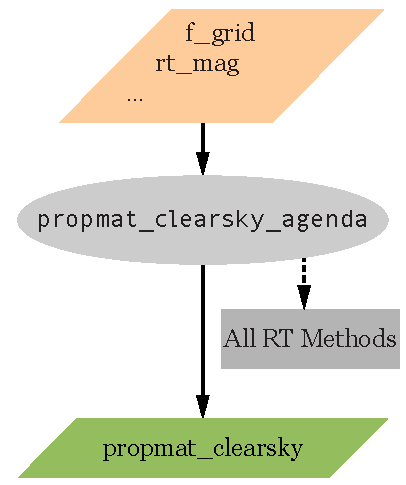
\includegraphics[scale=0.7]{propmat_clearsky_agenda}
  \caption{An outside view of propmat\_clearsky\_agenda.}
  \label{fig:absorption:pmat_outside}
 \end{center}
\end{figure}

The output of the agenda is a single variable,
\wsvindex{propmat\_clearsky}, a tensor with dimensions of absorption
species, frequency, Stokes dimension and Stokes dimension (Stokes
dimension of one thus emulates scalar absorption).  The physical
quantity corresponding to this variable is the clear-sky propagation
matrix \aAbsMat{a}\, as defined in Equation
\ref{eq:propmattotal}. It describes all non-scattering extinction
effects, that is, absorption and related polarization effects.

An inside view of propmat\_clearsky\_agenda is given in Figure
\ref{fig:absorption:pmat_inside}.  The agenda can contain a number of
different workspace methods that in some way or other compute
propmat\_clearsky. See the built-in documentation of the individual
methods to learn more. File \fileindex{agendas.arts}, one of the
standard include-controlfiles, predefines some typical alternatives
how propmat\_clearsky\_agenda can be set for different purposes.

\begin{figure}
 \begin{center}
  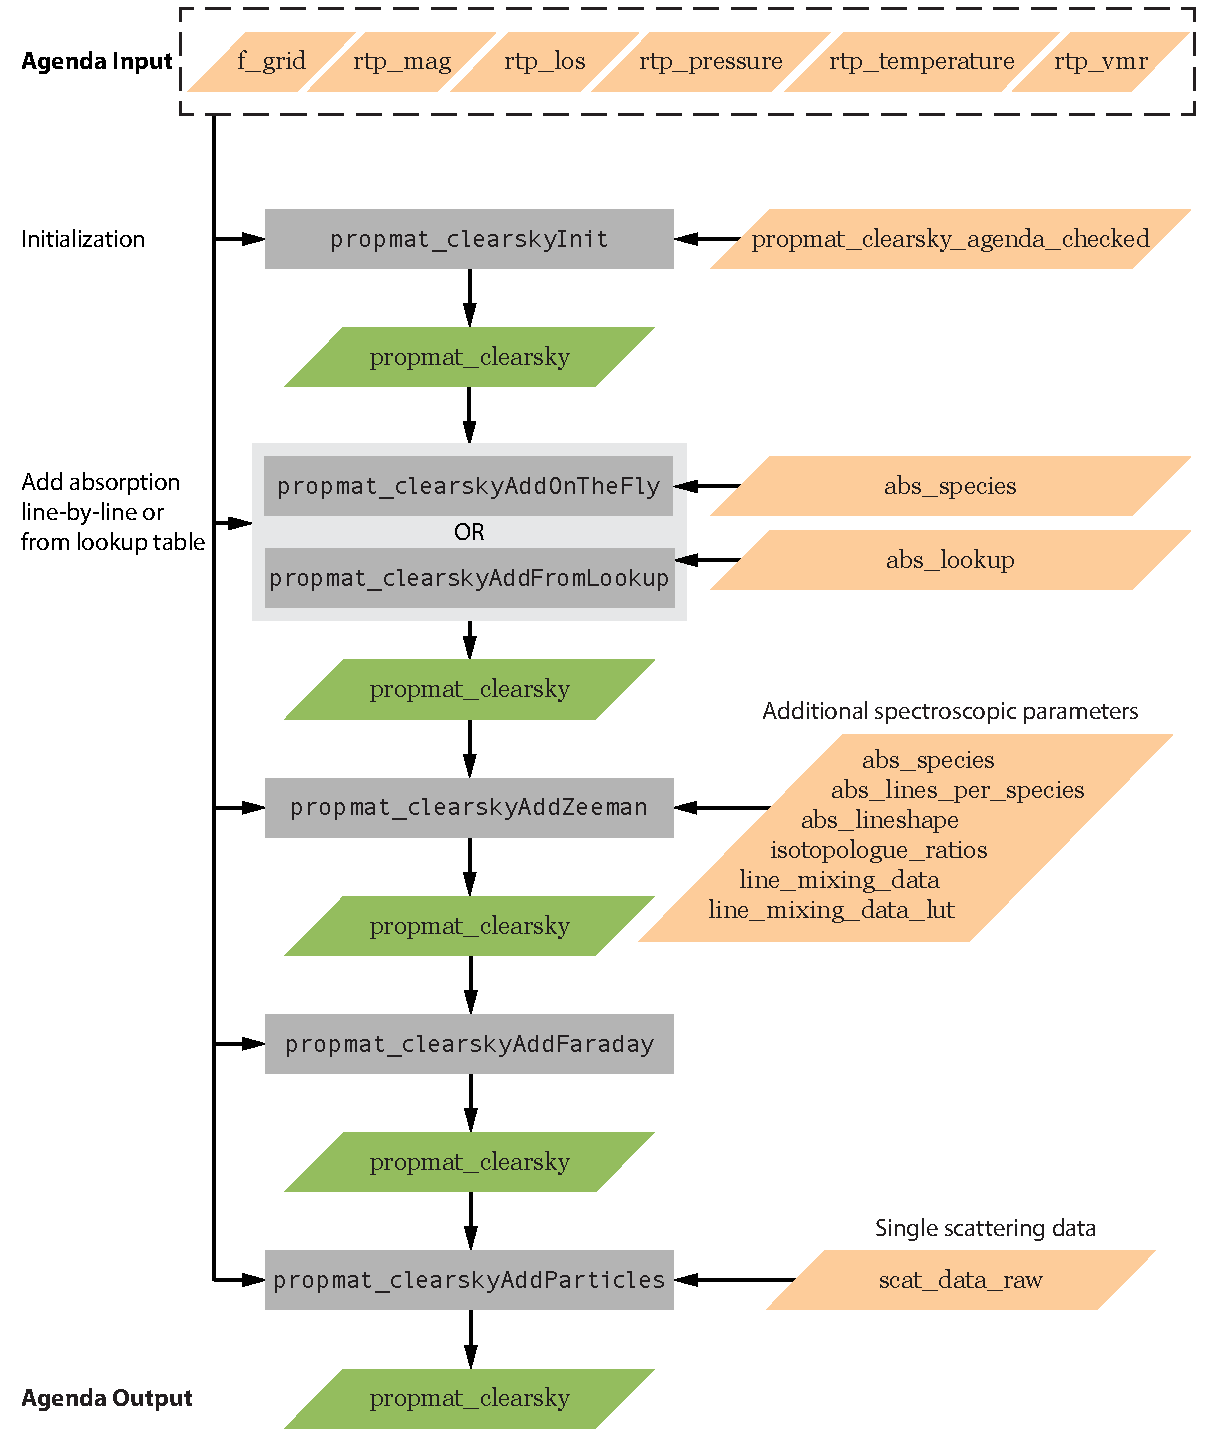
\includegraphics[scale=0.7]{propmat_clearsky_agenda_detail}
  \caption{An inside view of propmat\_clearsky\_agenda. At the same
    time, this gives an outside view of abs\_xsec\_agenda, as input to
    \wsmindex{propmat\_clearskyAddOnTheFly} in the context of
    on-the-fly absorption generation.}
  \label{fig:absorption:pmat_inside}
 \end{center}
\end{figure}



\section{Calculating gas absorption}
\label{sec:absorption:calculating}

This section deals with calculating gas absorption matrices in
ARTS.  This can typically occur in three different contexts:
as on-the-fly absorption matrix calculation within the radiative transfer
calculation,
% (see Section \ref{sec:absorption:abs-rt}), %this reference is more confusing than helping
when preparing
a gas absorption lookup table (see Section \ref{sec:absorption:lookup}),
or when the user is only interested in the absorption itself (see Section
\ref{sec:absorption:abs-only}).

In all these cases, the same agenda is used to actually calculate
absorption: abs\_xsec\_agenda. Outside views of this agenda are shown
in Figure \ref{fig:absorption:pmat_inside} (as input to
\wsmindex{propmat\_clearskyAddOnTheFly} in the context of on-the-fly
absorption generation) and Figure \ref{fig:absorption:xsec_in_lookup}
(as input to \wsmindex{abs\_lookupCalc} in the context of absorption
lookup table generation).

\begin{figure}
 \begin{center}
  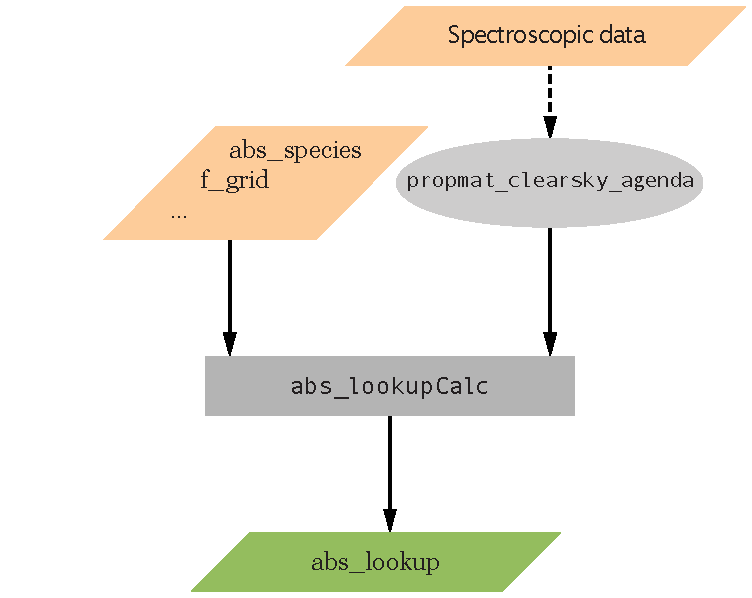
\includegraphics[scale=0.7]{abs_lookupCalc}
  \caption{An outside view of abs\_xsec\_agenda, in the context of
    absorption lookup table generation.}
  \label{fig:absorption:xsec_in_lookup}
 \end{center}
\end{figure}

An inside view of abs\_xsec\_agenda is given in Figure
\ref{fig:absorption:xsec_inside}.  The agenda can contain a number of
different workspace methods that in some way or other compute
abs\_xsec. See the built-in documentation of the individual methods to
learn more. As for propmat\_clearsky\_agenda, file
\fileindex{agendas.arts} predefines some typical alternatives also for
abs\_xsec\_agenda.

\begin{figure}
 \begin{center}
  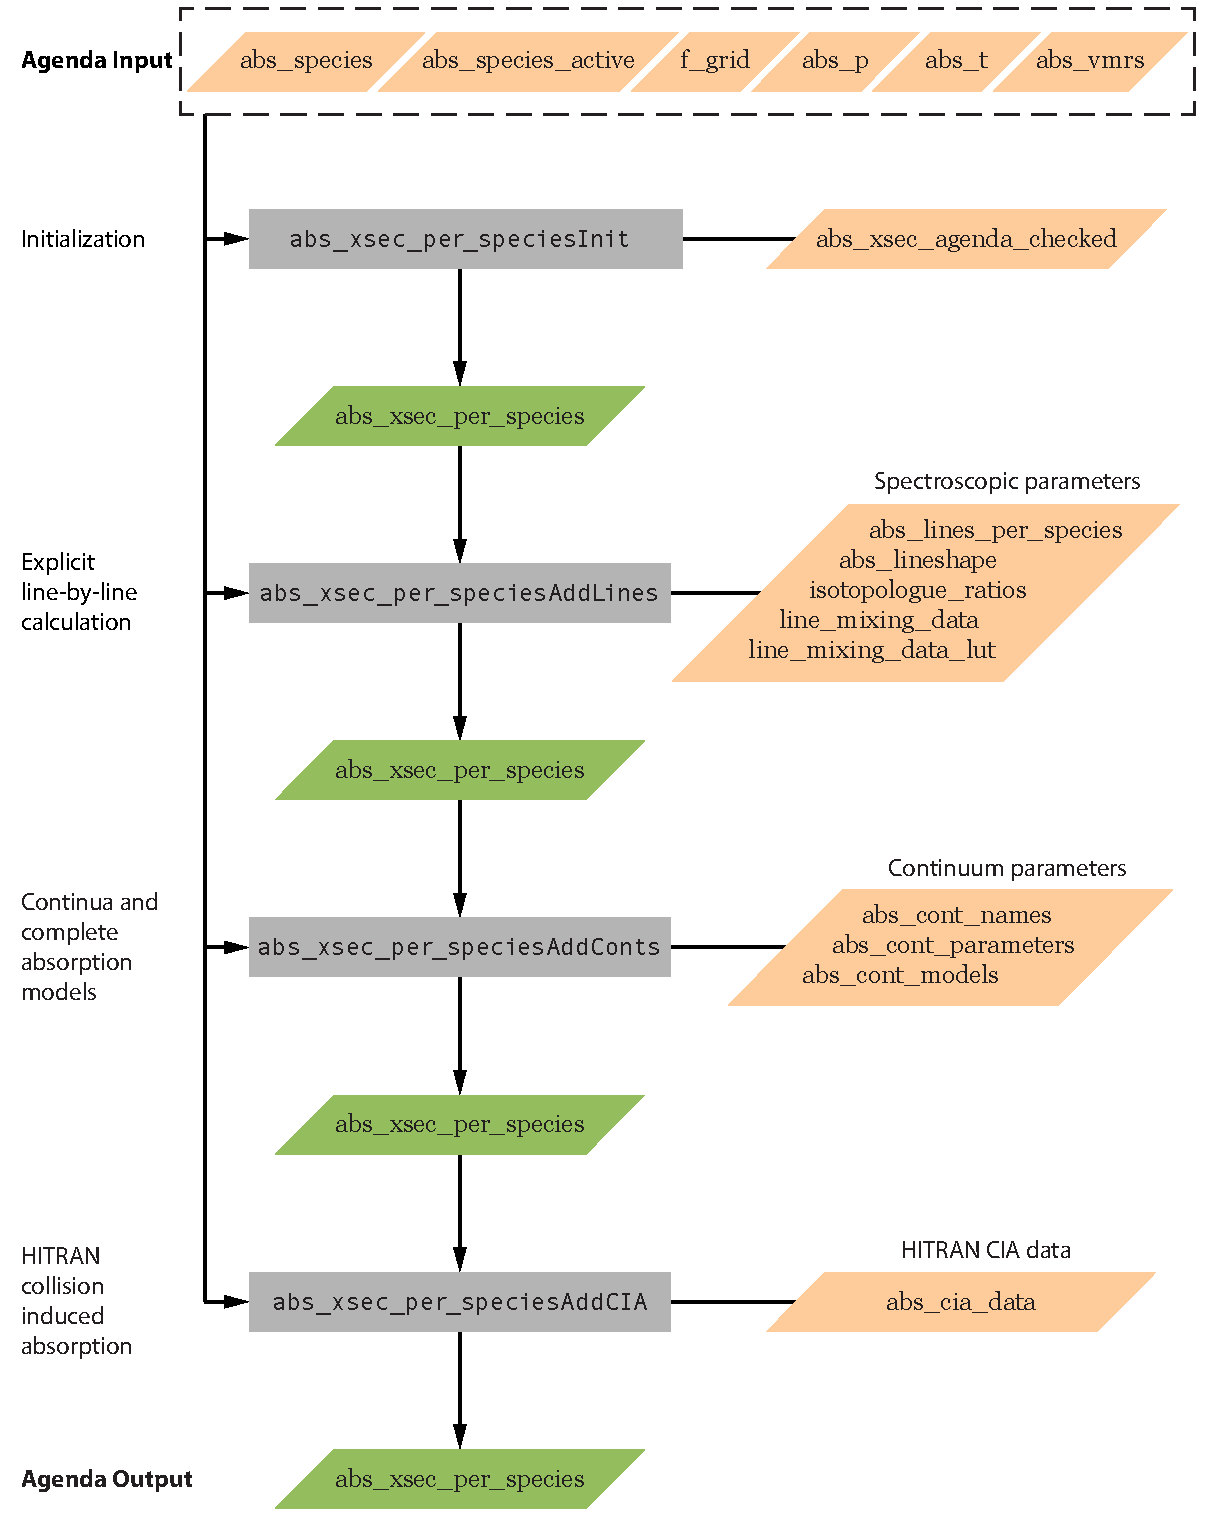
\includegraphics[scale=0.7]{abs_xsec_agenda}
  \caption{An inside view of abs\_xsec\_agenda.}
  \label{fig:absorption:xsec_inside}
 \end{center}
\end{figure}


\subsection{Absorption species}

Absorption is additive, so the total absorption is simply the sum of
all partial absorptions.  And the partial absorption for gases that
have spectral lines can be calculated as a sum over the absorption of
each spectral line, plus some more or less empirical continuum terms.

An absorption species in ARTS is an abstract entity that has a partial
absorption matrix associated with it, and that usually can be
associated with a volume mixing ratio of a corresponding gas (the VMRs
are stored in variable \wsvindex{vmr\_field}). Total absorption is the
sum of the partial absorptions of all absorption species. Absorption
species are defined in the ARTS controlfile by special `tags', which
are stored in the variable \wsvindex{abs\_species}, and set by the
method \wsmindex{abs\_speciesSet}.

The absorption species tags specify the different considered absorbers, which can
be gaseous species but also free electrons and (grey-body) particles.
For gaseous species, they also describe the model that should be used to
calculate the absorption for each of the species.
There are three types of tags, those for explicit line-by-line
calculations, those for continua and complete absorption models, and a special
Zeeman effect tag.
An example of the first kind is \verb|"H2O-18"|, which identifies a
particular isotopologue of water vapor. An example of the second kind is
\verb|"H2O-ForeignContCKDMT100"|, which identifies a particular continuum
model. An example of the third is \verb|"O2-Z"|, which identifies that special Zeeman
routines should be used.
Tags can be combined, if they refer to the same molecule
(different isotopologues are allowed). Even continuum tags can be combined
with explicit line-by-line tags, if they refer to the same molecule.

It should be noted that isotopologue ratios are taken into account
implicitly when line strengths are calculated, so even if you make
calculations for individual isotopologues, the VMR numbers in the
variable \wsvindex{vmr\_field} should not be adjusted for the isotopologue
ratio (the isotopologue ratio can be changed instead; see
Section~\ref{sec:absorption:isoratio}). As an example, to make a line-by-line
calculation for all ozone isotopologues, you could represent them in different
ways by
\wsmindex{abs\_speciesSet}.
\begin{code}
a) abs_speciesSet(species=["O3"])
b) abs_speciesSet(species=
                  ["O3-666, O3-668, O3-686, O3-667, O3-676"])
c) abs_speciesSet(species= 
                  ["O3-666", "O3-668", "O3-686", "O3-667", "O3-676"])
\end{code}
Options (a) and (b) are equivalent, you will have one ozone species
that represents all isotopologues, and that will be associated with a
single VMR field in \wsvindex{vmr\_field}.  With option (c) you have
five different ozone species, so you have to supply five different VMR
fields. If those five fields are identical (exactly same numerical
values), you will get the same total absorption as with options (a)
and (b).

Overall, the tag mechanism allows quite complex absorption setups. The built-in
documentation for \wsmindex{abs\_speciesSet} gives a detailed explanation of the
tag syntax and some examples.

Particularly note, that order of the species list matters as absorption line
data is assigned to species in their order within the \wsvindex{abs\_species}
list and no line record is assigned to more than one species.
It is furthermore important to note that there is no `intelligence' in ARTS that
checks that the chosen tag combinations make sense, so the user should
know what s/he is doing, or follow one of the many examples in
the ARTS \fileindex{controlfiles} directory.

\subsection{Explicit line-by-line calculations}

For absorption species with explicit line-by-line calculation the
calculation involves the steps summarized in Table
\ref{tab:absorption:lbl}, which contains the steps that are common to all the
three contexts in which explicit line-by-line calculations can occur as well
as the steps that are specific to each of those cases. 
The list of variables and methods in the
table is not complete. The idea is to give an overview over the
important ones and show how they work together. Missing are
particularly the input variables that describe the atmospheric
conditions, and continuum description variables, which normally do not
have to be set by the user anyway.

\begin{table}
\footnotesize
\renewcommand{\arraystretch}{1.5}
\newcounter{rownum}
\newcommand{\mylabel}[1]{\refstepcounter{rownum} \label{#1}}
\begin{tabularx}{\hsize}{l>{\raggedright\arraybackslash\hsize=0.5\hsize}X
                          >{\raggedright\arraybackslash\hsize=1.5\hsize}X}
\hline
\# & Step & Variables and Methods \\
\hline
%---------------------------------------------------------------------
\mylabel{step:lineshape}
\arabic{rownum} & 
Define line shape function(s) to use. &
Variable:
\wsvindex{abs\_lineshape}. \newline
Methods:
\wsmindex{abs\_lineshapeDefine} (same shape for all species),
\wsmindex{abs\_lineshape\_per\_tgDefine} (different shapes for different
species). \\
%---------------------------------------------------------------------
\mylabel{step:readline}
\arabic{rownum} &
Read spectral line data (the order of the first two steps does not
matter). &
Variable: \wsvindex{abs\_lines}. \newline
Methods: 
\wsmindex{abs\_linesReadFromArts},
\wsmindex{abs\_linesReadFromSplitArtscat},
\wsmindex{abs\_linesReadFromHitran},
\wsmindex{abs\_linesReadFromHitranPre2004},
\wsmindex{abs\_linesReadFromJpl},
\wsmindex{abs\_linesReadFromMytran2} (different methods are for
different catalogue formats). For the ARTS internal format, the
standard method \wsmindex{ReadXML} works also, but does not allow to
select a frequency range, as the others do. \\
%---------------------------------------------------------------------
\mylabel{step:splitline}
\arabic{rownum} &
Split line data for different absorption species. &
Variable: \wsvindex{abs\_lines\_per\_species}. \newline
Methods:
\wsmindex{abs\_lines\_per\_speciesCreateFromLines}. Alternatively, read
lines from different catalogues for different species directly with
\wsmindex{abs\_lines\_per\_speciesReadFromCatalogues}. \\
%---------------------------------------------------------------------
\mylabel{step:optline}
\arabic{rownum} &
Optimize line data. (optional)&
Variable: \wsvindex{abs\_lines\_per\_species}. \newline
Methods: Add mirror lines for VVW line shape with
\wsmindex{abs\_lines\_per\_speciesAddMirrorLines} (see \theory,
Chapter \ref{T-sec:abs_theory}). Remove lines that are outside the
line shape cutoff with \wsmindex{abs\_lines\_per\_speciesCompact}. \\
%---------------------------------------------------------------------
\multicolumn{3}{>{\raggedright\arraybackslash\hsize=2\hsize}X}{The
  first four steps are preparation, and typically 
  have to be done only once per ARTS run. The fifth step is the actual
  absorption calculation, which can occur in different contexts.} \\
%---------------------------------------------------------------------
\mylabel{step:calc}
\arabic{rownum}a &
Calculate absorption on-the-fly. &
Agenda: \wsaindex{propmat\_clearsky\_agenda}. \newline
Variable: \wsvindex{propmat\_clearsky}, which is nitialized in \wsmindex{propmat\_clearskyInit}.\newline
Methods: \wsmindex{propmat\_clearskyAddOnTheFly} (the core method for on-the-fly
absoprtion calculation inlcuding line-by-line and continuum absorption), \newline
\wsmindex{propmat\_clearskyAddZeeman} (see Sec.~\ref{sec:absorption:zeeman}), \newline
\wsmindex{propmat\_clearskyAddFaraday} (see Sec.~\ref{sec:absorption:faraday}), \newline
\wsmindex{propmat\_clearskyAddParticles} (see Sec.~\ref{sec:absorption:particles}). \newline
Alternative:
\wsmindex{propmat\_clearskyAddFromLookup} instead of \wsmindex{propmat\_clearskyAddOnTheFly}
(extract absorption from pre-calculated lookup table, see
Sec.~\ref{sec:absorption:lookup}). Note that the lookup
table cannot contain absorption for Zeeman tagged species, Faraday rotation, and
particles due to their directional dependencies.\\
%---------------------------------------------------------------------
\arabic{rownum}b &
Calculate absorption lookup table. &
Variable: \wsvindex{abs\_lookup}. \newline
Methods: \wsmindex{abs\_lookupCalc}. Alternative: Load lookup table
from file with \wsmindex{ReadXML}, it then has to be adapted to the
current calculation (and checked) with \wsmindex{abs\_lookupAdapt}. \\ 
%---------------------------------------------------------------------
\arabic{rownum}c &
Calculate absorption only (no RT). &
Variable: \wsvindex{propmat\_clearsky\_field}, \wsvindex{abs\_coef}. \newline
Methods, high level: \wsmindex{propmat\_clearsky\_fieldCalc}. \newline
Methods, low level: \newline
\wsmindex{abs\_xsec\_per\_speciesInit}, \newline
\wsmindex{abs\_xsec\_per\_speciesAddLines} (the core method for the
actual line-by-line calculation, used internally by all higher level methods),\newline
\wsmindex{abs\_xsec\_per\_speciesAddConts} (add continua or complete absorption
models, see Section \ref{sec:absorption:continua}),\newline
\wsmindex{abs\_xsec\_per\_speciesAddCIA} (add collision induced absorption, see
Section \ref{sec:absorption:cia}),\newline
\wsmindex{abs\_coefCalcFromXsec} (calculate absorption coefficients
from absorption cross-sections). \\
%---------------------------------------------------------------------
\hline
\end{tabularx}
\caption{Steps for line-by-line absorption calculation, and associated
    ARTS workspace variables and methods.}
\label{tab:absorption:lbl}
\end{table}

See the built-in documentation of the various variables and methods
for more information.  It is on purpose not repeated here, for better
maintainability.  If you are viewing this pdf file on a computer, just
click on a variable or method name to get to the corresponding
built-in documentation. Further input data and parameters required (not only)
for line-by-line calculations is described in Section~\ref{sec:absorption:input}.

\subsection{Continua and complete absorption models}
\label{sec:absorption:continua}

ARTS includes many absorption continua and complete absorption models,
which are described in \theory, Chapter \ref{T-sec:abs_theory}.  The
common property of all of these is that they do not use the standard
ARTS line-by-line calculation mechanism.  They may include spectral
lines, but then these lines are hardwired into the absorption model
itself.  Consequently, the first four steps in Table
\ref{tab:absorption:lbl} are not needed for these models.  

The pure continua are intended to be used together with an explicit ARTS
line-by-line calculation, the complete models are intended to be used alone.
To select a continuum or complete absorption model, simply use the
corresponding tag with \wsmindex{abs\_speciesSet}.  Currently available
models are listed in Table \ref{tab:absorption:continua}.

\begin{table}
\centering
\footnotesize
\begin{tabular}{ll}
\hline  
Class & Tag name \\
\hline  
%---------------------------------------------------------------------

Water vapor continua
& H2O-SelfContStandardType \\
& H2O-ForeignContStandardType \\
& H2O-ForeignContMaTippingType \\
& H2O-ContMPM93 \\
& H2O-SelfContCKD222 \\
& H2O-ForeignContCKD222 \\
& H2O-SelfContCKD242 \\
& H2O-ForeignContCKD242 \\
& H2O-SelfContCKD24 \\
& H2O-ForeignContCKD24 \\
& H2O-SelfContCKDMT100 \\
& H2O-ForeignContCKDMT100 \\
& H2O-SelfContCKDMT252 \\
& H2O-ForeignContCKDMT252 \\
& H2O-ForeignContATM01 \\[1ex]

Complete water vapor models
& H2O-CP98 \\
& H2O-MPM87 \\
& H2O-MPM89 \\
& H2O-MPM93 \\
& H2O-PWR98 \\[1ex]

Carbon dioxide continua 
& CO2-CKD241 \\
& CO2-CKDMT100 \\
& CO2-CKDMT252 \\
& CO2-SelfContPWR93 \\
& CO2-ForeignContPWR93 \\
& CO2-SelfContHo66 \\
& CO2-ForeignContHo66 \\[1ex]

Oxygen continua 
& O2-CIAfunCKDMT100 \\
& O2-v0v0CKDMT100 \\
& O2-v1v0CKDMT100 \\
& O2-visCKDMT252 \\
& O2-SelfContStandardType \\
& O2-SelfContMPM93 \\
& O2-SelfContPWR93 \\[1ex]

Complete oxygen models & O2-PWR98 \\
& O2-PWR93 \\
& O2-PWR88 \\
& O2-MPM93 \\
& O2-MPM92 \\
& O2-MPM89 \\
& O2-MPM87 \\
& O2-MPM85 \\
& O2-TRE05 \\[1ex]

Nitrogen continua & N2-SelfContMPM93 \\
& N2-SelfContPWR93 \\
& N2-SelfContStandardType \\
& N2-SelfContBorysow \\
& N2-CIArotCKDMT100 \\
& N2-CIAfunCKDMT100 \\
& N2-CIArotCKDMT252 \\
& N2-CIAfunCKDMT252 \\
& N2-DryContATM01 \\[1ex]

Condensate absorption models & liquidcloud-MPM93 \\
& icecloud-MPM93 \\
& rain-MPM93 \\

%---------------------------------------------------------------------
\hline  
\end{tabular}
\caption{ARTS continua and complete absorption models. The molecular
  species can be inferred from the start of the tag name.  See
  \theory, Chapter \ref{T-sec:abs_theory} for more information on the
  various models.}
\label{tab:absorption:continua}
\end{table}

The names should be fairly self-explanatory and can be used to find
background information on the various models in \theory.  The
condensate absorption models are a bit special and perhaps need some
extra explanation. They are absorption parameterizations by Liebe, and
allow the inclusion of condensate in the (rare) cases where scattering
is not important. Their general applicability is therefore fairly limited.

The behavior of the continua and complete absorption models can be
modified by passing them some additional parameters, stored in the
variables \wsvindex{abs\_cont\_names}, \wsvindex{abs\_cont\_models},
and \wsvindex{abs\_cont\_parameters}. Basically,
\builtindoc{abs\_cont\_names} identifies the model,
\builtindoc{abs\_cont\_models} contains switches that select different
behavior (for example taking only the lines, or only the continuum
part of a complete model), and \builtindoc{abs\_cont\_parameters} can
contain numerical parameters. 

Yes, the nomenclature for these additional continuum parameters,
particularly \builtindoc{abs\_cont\_models}, is confusing. However,
most users will never have to deal with these variables
explicitly. They are set to default values in the include file
\fileindex{continua.arts}. Users should therefore always include this file  at
the start of their controlfiles with
\begin{code}
  INCLUDE "continua.arts"
\end{code}
Unless you work on continuum model development or verification, you
should never have to modify these default settings.

The core method to calculate continua and complete absorption models
is \wsmindex{abs\_xsec\_per\_speciesAddConts}.  Users normally do not
have to call this method explicitly, since it is used implicitly by
higher level methods, such as \wsmindex{propmat\_clearskyAddOnTheFly} and
\wsmindex{propmat\_clearsky\_fieldCalc}.

\subsection{Collision-induced absorption}
\label{sec:absorption:cia}

Collisions of centro-symmetric molecules, e.g., \chem{O_2},
\chem{N_2}, \chem{H_2}, \chem{CO_2}, and \chem{CH_4}, possessing no permanent
electric dipole create a transient dipole, which causes so-called collision-induced
absorption (CIA). Absorption strength of CIA is characterized by its dependency
on the molecular density of both molecular species involved in the collision.

Recently, the well-known HITRAN spectral line catalogue has started to
offer also tabulated binary absorption cross-sections for CIA.  This is
described in detail in \citet{richard:12}, and also in the documentation that
comes with the data themselves.

Binary absorption cross-sections
\aAbsXsec{i,j} have to be multiplied with the number densities of both involved
molecular species to yield absorption coefficients:
\begin{equation}
\aAbsCoef{i,j} =  \aAbsXsec{i,j} \, \aDen{i} \, \aDen{j},
\end{equation}
where $i$ and $j$ denote the two different absorbing species. As a
consequence, \aAbsXsec{i,j} has units of m$^5$/molec$^2$ in ARTS (the
original HITRAN units are different).

Using CIA in ARTS is easy. First of all, include one or more CIA tags
in your absorption species list (\wsvindex{abs\_species}). All valid
tags are listed in Table \ref{tab:absorption:cia_ranges}. Secondly,
read in WSV \wsvindex{abs\_cia\_data}, which contains the tabulated
binary absorption cross-sections, from a file. This will usually be the
file \fileindex{hitran\_cia2012\_adapted.xml.gz}, which is included in the
\shortcode{arts-xml-data}, but the original HITRAN data files can also be
read. Finally, use WSM \wsmindex{abs\_xsec\_per\_speciesAddCIA} in
abs\_xsec\_agenda to add the CIA absorption. For usage examples, look
in directory \fileindex{controlfiles/artscomponents/cia} that is part
of the ARTS distribution.

Figure \ref{fig:absorption:cia} shows all CIA continua that are
currently available in ARTS (left) and separately the ones that are
relevant for Earth's atmosphere (right). The valid frequency and
temperature ranges for these data, as available in ARTS, are listed in
Table \ref{tab:absorption:cia_ranges}. Outside the covered frequency ranges, the
binary absorption cross-sections are set to zero, while exceeding the valid
temperature range will produce \verb|NaN| values and eventually trigger a
runtime error.

To make the HITRAN data work in ARTS, some modifications were necessary,
specifically:

\begin{description}
\item[N$_2$-N$_2$:] The two high-frequency datasets were merged into one.
\item[O$_2$-O$_2$:] Three apparently separate datasets that really
  belong together were merged. UV/Vis dataset were removed.
\item[CO$_2$-CO$_2$:] Caveat: This is only the self continuum of
  CO2. The CO2-air continuum has strong features above 250\,cm$^{-1}$ that
  are present in CKD\_MT (also available in ARTS as one of the
  continuum and full absorption models), but are missing here.
  %The HITRAN data also generally looks weird. It is only in the alternative
  %folder, and \citet{richard:12} basically recommend not to use it. Conclusion:
  %No changes, but usage not recommended.
  Furthermore, \citet{richard:12} point out that for molecules with more than two atoms
  further mechanisms affecting CIA exist, which are not covered by the simple
  models used. They hence state that ``these data should be used very
  carefully''. Conclusion: No changes, but use with care.

  Also note that no data exists at frequencies below 30\,GHz (1\,cm$^{-1}$)
  though some significant absorption is still present at the limiting frequency.
  For those low frequencies, the CO2-SelfContPWR93 continuum (see
  Table~\ref{tab:absorption:continua}) can be used as an alternative (we
  estimated that to be valid at least up to about 100\,GHz, but deviating
  significantly above 500\,GHz).
\item[O2-N2, O2-CO2:] These UV/Vis-only datasets were removed.

\begin{table}
    \caption{Absorption species tags, frequency ranges, and
      temperature ranges for HITRAN CIA data as implemented in
      ARTS. (These data contain some modifications from the original
      HITRAN data, which are described in the text.)} 
    \label{tab:absorption:cia_ranges}
    \centering
    \begin{tabular}{llll}
\hline
    CIA tag& Spectral range [cm$^{-1}$]& Temp range [K]& No. of datasets\\
\hline
  N2-CIA-N2-0& 0.02 -- 554.00& 40.00 -- 400.00& 10\\
  N2-CIA-N2-1& 1850.00 -- 3000.09& 228.20 -- 362.50& 10\\
  N2-CIA-H2-0& 0.02 -- 1886.00& 40.00 -- 400.00& 10\\
  N2-CIA-CH4-0& 0.02 -- 1379.00& 40.00 -- 400.00& 10\\
  H2-CIA-H2-0& 20.00 -- 10000.00& 200.00 -- 3000.00& 113\\
  H2-CIA-He-0& 20.00 -- 20000.00& 200.00 -- 9900.00& 334\\
  H2-CIA-CH4-0& 0.02 -- 1946.00& 40.00 -- 400.00& 10\\
  H2-CIA-H-0& 100.00 -- 10000.00& 1000.00 -- 2500.00& 4\\
  He-CIA-H-0& 50.00 -- 11000.00& 1500.00 -- 10000.00& 10\\
  O2-CIA-O2-0& 1150.00 -- 1950.00& 193.40 -- 353.40& 15\\
  CO2-CIA-CO2-0& 1.00 -- 250.00& 200.00 -- 800.00& 7\\
  CH4-CIA-CH4-0& 0.02 -- 990.00& 40.00 -- 400.00& 10\\
  CH4-CIA-Ar-0& 1.00 -- 697.00& 70.00 -- 296.00& 5\\
\hline
\end{tabular}
\end{table}


\end{description}

\begin{figure}
 \begin{center}
  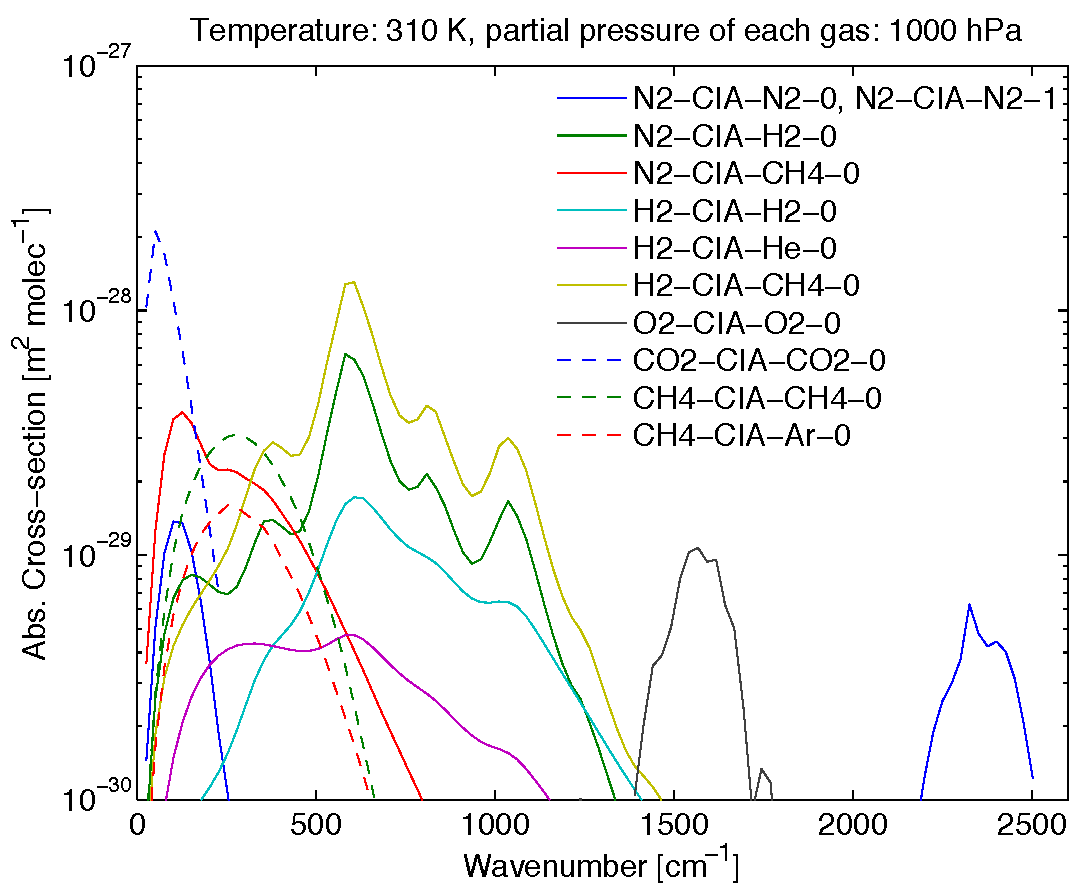
\includegraphics[width=.46\hsize]{plot_all_arts_cia_generic_1}
  \hspace{\fill}
  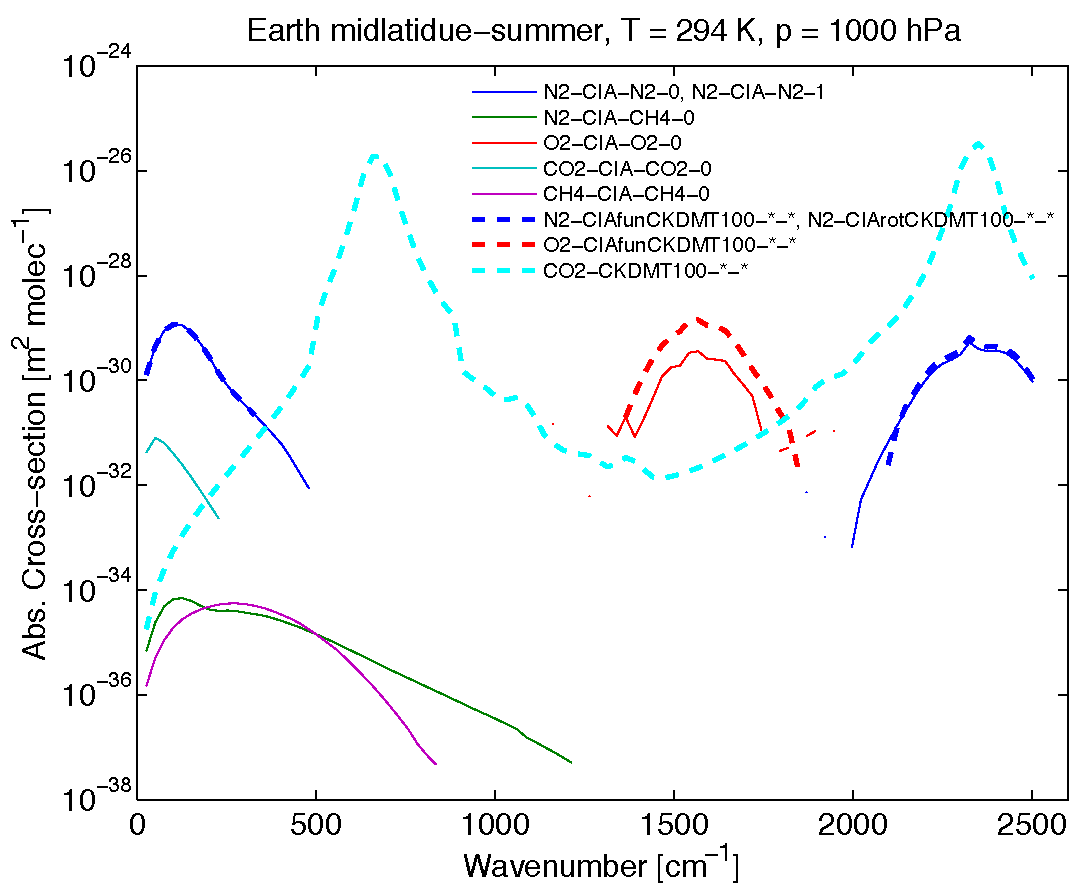
\includegraphics[width=.46\hsize]{plot_earth_continua_1_1}
  \caption{Left: All HITRAN CIA continua that are implemented in ARTS
    (each gas here has a partial pressure of 1000\,hPa). Right: Only
    the ones that are relevant for Earth (for Earth surface
    conditions).}
  \label{fig:absorption:cia}
 \end{center}
\end{figure}

\subsection{Zeeman calculations}
\label{sec:absorption:zeeman}

The Zeeman effect is calculated in the method \wsmindex{propmat\_clearskyAddZeeman}.
If this method is included in the \builtindoc{propmat\_clearsky\_agenda}, then species with the
tag "\verb|-Z|" will be calculated as Zeeman species. If the method is not included,
then these species will simply be ignored. Note that the order within the tag
string is important: the Zeeman tag must directly follow the molecular species
tag. That is, \verb|O2-Z-66| will be counted as Zeeman splitting on the
O$^{16}$O$^{16}$ molecule, whereas \verb|O2-66-Z| will not work the same way, or even at all.

The physics and internal workings of the Zeeman calculations follow the scheme
presented in \citet{larsson:xx} %FIXME: update bibtex reference when accepted.
%Larsson et al., submitted 2013 to JQSRT, \textit{A treatment of the Zeeman
%effect using Stokes formalism and its implementation in the Atmospheric
%Radiative Transfer Simulator ARTS}.

In order to calculate Zeeman splitting, additional line parameters that are not
readily available in, e.g., HITRAN are necessary. These include $g_s$ [-], the
relative Land\'{e} factor, and $S$ [-], the molecular total spin. These
variables must therefore be read to the WSV \wsvindex{isotopologue\_quantum}.
This variable is of type \builtindoc{SpeciesAuxData}, and a file providing
that kind of data would, e.g., look like:
\begin{code}
<arts format="ascii" version="1">
  <SpeciesAuxData version="1" nelem="1" nparam="3">
    @ O2-66 2.002064 1 1
  </SpeciesAuxData>
</arts>
\end{code}
In this example, \verb|@| indicates the beginning of a new data record, \verb|O2-66|
specifies what isotopologue is associated with the data, the number
\verb|2.002064| is the relative Land\'{e} factor, and the molecule got $S=1$.
The last value indicates what Hund case is used in the calculations. For oxygen,
Hund case b is used, indicated b the number "1". Presently, Hund case a, indicated
by number "0" also works for some molecules. It is up to the user to assure the
correct quantum numbers for each case are set properly.
The supported molecules in ARTS so far for Zeeman calculations are
\begin{itemize}
\item O$_2$, case b
\item NO, case a/b
\item OH, case a
\item ClO, case a
\item HO$_2$, case b
\item NO$_2$, case b
\end{itemize}
but only O$_2$ is tested beyond initial modeling results.

Beside the additional line parameters, it is also necessary to input the magnetic
field into the model. This can be done following:
\begin{code}
GriddedField3Create(B)
  ReadXML(B,"B_1comp.xml.gz")
  GriddedFieldLatLonRegrid( B, lat_grid, lon_grid, B )
  GriddedFieldPRegrid( B, p_grid, B )
  FieldFromGriddedField( mag_w_field, p_grid, lat_grid, 
                         lon_grid, B )
\end{code}
where \verb|B_1comp.xml.gz| contains the (atmospheric) profile or field for one
components of the magnetic field. 
Since the magnetic field is usually not dependent on the pressure,
it is also possible to use the  
\begin{code}
 GriddedFieldZToPRegrid(*)
\end{code}
functionality to input altitude-gridded magnetism.
Input needs to be provided for each non-zero
magnetic field component separately into the respective WSVs \wsvindex{mag\_w\_field}, 
\wsvindex{mag\_v\_field}, and \wsvindex{mag\_u\_field}. For more information on
magnetic field format in ARTS see Section~\ref{sec:atm:vecfields}.

Lastly, it is necessary to take phase effects into account when calculating the
Zeeman effect. It is therefore important that \wsvindex{abs\_lineshape} is
chosen such that it allows for this information to be provided. One
suitable line shape can be defined through
\begin{code}
abs_lineshapeDefine( abs_lineshape, "Faddeeva_Algorithm_916", 
                     "VVH", 750e9 )
\end{code}

\subsection{Internal line-mixing}
\label{sec:absorption:line-mixing}

Line mixing is implemented as the \verb|-LM-| species tag.  Added to 
a species, ARTS knows that it should look for lines with
line mixing data attached to them when it calculates the spectral cross sections.
Note that each line is initialized without any line mixing data, and with a tag 
state that says they are not to be line mixed.  If this is not changed before the
absorption calculations are performed, the line will regardless of species tag still
act like if it were not line mixed.  Also note that it is possible to calculate line mixing
in conjuncture with the Zeeman effect, but that it is not possible to calculate the line mixing
of individual Zeeman lines, which as far as we know when writing this is unimportant.

The possible tags on species \verb|X| that activates the line mixing module are thus
\verb|X-LM-*|, and \verb|X-Z-LM-*|.
The supported ways to ensure that the line record contains information on
how to calculate line mixing, thus not ignoring it, are 
\begin{itemize}
 \item Read an ARTS catalogue file with line mixing parameters.
 \item Read LBLRTM line catalogue containing line mixing parameters using 
 \verb|abs_linesReadFromLBLRTM(*)|.
 \item Read a line database that does not have line mixing, but use the 
 \verb|line_mixing_dataMatch(*)| method to inject line mixing data into the line record.
\end{itemize}
There is no preferred method in ARTS --- each work the same when they reach the absorption
calculations --- but we urge the user to be sure that line mixing data and the line database
are of the same origin, as the calculations will be of poor quality if this is not the case.

Example control file meta flow for code calculating line mixing using \verb|abs_linesReadFromLBLRTM|:
\begin{code}
# Define your atmospheric species,
abs_speciesSet(species=["O2-Z-LM","CO2-LM"])

# read from a line database,
abs_linesReadFromLBLRTM(filename="aer", 
    fmin=1e1,fmax=1e20)
\end{code}
Note that this meta flow is very similar to using an ARTS catalogue with line mixing.
These methods are easy, because they identity what line mixing method will be used 
directly from the catalogue.
It should be noted that LBLRTM also gives the non-resonant term of the molecular oxygen
spectra as a low frequency line.  If it is desired to calculate this term, the lower
frequency range must contain the line as per the definition of our reading routines.

Example control file meta flow for code calculating line mixing using \verb|line_mixing_dataMatch|:
\begin{code}
# Define your atmospheric species,
abs_speciesSet(species=["O2-Z-LM","CO2-LM"])

# Read from a line database,
abs_linesReadFromHITRAN(filename="HITRAN2012.par", 
    fmin=1e1,fmax=1e20)

# Sort the line records into the format ARTS wants
abs_lines_per_speciesCreateFromLines

# Create a way to temporally store O2 line mixing data.
ArrayOfLineMixingRecordCreate(lm_o2)
ReadXML(lm_o2,"o2.xml")

# Create a way to temporally store CO2 line mixing data.
ArrayOfLineMixingRecordCreate(lm_co2)
ReadXML(lm_co2,"co2.xml")

# Match the line mixing data with O2 and Zeeman effect
line_mixing_dataMatch(
    species_tag="O2-Z-LM",
    line_mixing_records=lm_o2
    line_mixing_tag=LM*)

# Match the line mixing data with O2 and Zeeman effect
line_mixing_dataMatch(
    species_tag="CO2-LM",
    line_mixing_records=lm_co2,
    line_mixing_tag=LM*)
\end{code}
The latter method is much more complicated than reading directly from the catalogue.
This is because the user has to ensure what type of line mixing is going on
and then parse that data properly to ARTS.  In order for ARTS to know what line the user 
wants to line mix, a series of line database matching 
based on the quantum numbers of the line is necessary.
This means that it only works for those species and catalogue formats
for which we have implemented quantum number reading.
This list is small but growing, and if you need help adding another species, 
let us know via the mailing list.

There are three \verb|line_mixing_tag| supported at this point:
\verb|"LL"|, \verb|"NR"| and \verb|"L2"|.  These refer to LBLRTM, and second order line mixing.
Setting these tags will tell ARTS how to calculate the line mixing of any particular line.
The data is matched from \verb|ArrayOfLineMixingRecord|,
which must contain a \verb|SpeciesTag|, a
\verb|QuantumNumberRecord|, and a vector that is the correct length for the method selected

Example of correct input data for using the second order approach ("L2"):
\begin{code}
<?xml version="1.0"?>
<arts format="ascii" version="1">
<Array type="LineMixingRecord" nelem="38">
<LineMixingRecord>
<SpeciesTag>"O2-66-*-*"</SpeciesTag>
<QuantumNumberRecord>
<Upper><QuantumNumbers nelem="3"> 
  J 1/1 N 1/1 v1 0/1 
</QuantumNumbers></Upper>
<Lower><QuantumNumbers nelem="3"> 
  J 2/1 N 1/1 v1 0/1 
</QuantumNumbers></Lower>
</QuantumNumberRecord>
<Vector nelem="10">
2.65e-06
-1.32e-07
-8.35e-12
8.43e-13
0.000545
0.00017
300
0.8
1.6
1.6
</Vector>
</LineMixingRecord>
</Array>
</arts>
\end{code}
The format of the above data is thusly: \shortcode{SpeciesTag},
\shortcode{QuantumNumberRecord}, \shortcode{Vector}, 
The above input will cause the \verb|O2-66-*-*| line with
upper quantum numbers $J=1$, $N=1$ and $\nu_1=0$ and with
lower quantum numbers $J=2$, $N=1$ and $\nu_1=0$ to match.
If this is the only input file, the described line is the only
line experiencing line mixing in your calculations. If there
were more lines in the file, these would also experience line mixing.
In order of appearance in the vector, its format is 
first order zeroth phase correction [Pa$^{-1}$], 
first order first phase correction [Pa$^{-1}$],
second order zeroth absorption correction [Pa$^{-2}$],
second order first absorption correction [Pa$^{-2}$],
second order zeroth line-center correction [Hz Pa$^{-2}$],
second order first line-center correction [Hz Pa$^{-2}$],
standard temperature for corrections [K],
first order phase temperature correction exponential term [-],
second order absorption temperature correction exponential term [-], and
second order line-center temperature correction exponential term [-].
The format of the vector is fixed according to necessary information found 
in \citet{makarov11:_60-ghz_jqsrt},
the naming scheme of the variables above can also be understood from the same work.
Note that first order line mixing, as per the MPM/PWR complete oxygen models, 
can be achieved with the correct input by letting the second order terms be nil.



Example of correct input data for using the LBLRTM approach ("LL" and "NR"):
\begin{code}
<?xml version="1.0"?>
<arts format="ascii" version="1">
<Array type="LineMixingRecord" nelem="38">
<LineMixingRecord>
<SpeciesTag>"O2-66-*-*"</SpeciesTag>
<QuantumNumberRecord>
<Upper><QuantumNumbers nelem="3"> 
  J 1/1 N 1/1 v1 0/1 
</QuantumNumbers></Upper>
<Lower><QuantumNumbers nelem="3"> 
  J 2/1 N 1/1 v1 0/1 
</QuantumNumbers></Lower>
</QuantumNumberRecord>
<Vector nelem="12">
200
250
296
340
-0.004433034295584e-4
-0.003982500863558e-4
-0.003628075993092e-4
-0.003341074759437e-4
0
0
0
0
</Vector>
</LineMixingRecord>
</Array>
</arts>
\end{code}
In this format, the first four values are a temperature grid in Kelvin.
For "LL" the following four values are the first order
line mixing coefficients at these temperature grid points [in units 1/Pa], 
and the last four are the second order line mixing coefficients at these temperature grid points [in units 1/Pa$^2$].
For "NR" the following four values are the first order
non-resonant term at these temperature grid points [in units 1/Pa], 
and the last four are the second order non-resonant terms
at these temperature grid points [in units 1/Pa$^2$].
ARTS will use linear interpolation to get proper coefficients between and slightly outside grid points.

\textit{Warning:} There appears to be some errors in the quantum number encoding
in HITRAN04 and HITRAN08 that makes the line mixing module wrong.  The newer
HITRAN2012 has fixed these issues.

\subsection{Faraday rotation}
\label{sec:absorption:faraday}

Faraday rotation is a change of polarization state of radiation in interaction
with (free) electrons in presence of a static magnatic field. For further
details on theory and usage in ARTS see Section~\ref{sec:faraday}.
Here we only give a short summary how to setup the calculation of Faraday
contribution to the absorption (or better: propagation) matrix
\wsvindex{propmat\_clearsky}.

First, to include Faraday rotation effects
\wsmindex{propmat\_clearskyAddFaraday} must be included in the
\builtindoc{propmat\_clearsky\_agenda}. Second, a species tag
\verb|"free_electrons"| needs to be contained in \wsvindex{abs\_species}.
Correspondingly, a field of electron densities is required in
\builtindoc{vmr\_field}.

For usage examples, check \fileindex{controlfiles/artscomponents/faraday} that
is part of the ARTS distribution.

\subsection{Absorbing particles}
\label{sec:absorption:particles}

% what are particles doing here? what for / when is this useful?
As pointed out before, this chapter deals with absorption by non-scattering
matter. In first place this refers to gases, while particles (aerosols, clouds,
precipitation) are considered to (also) scatter radiation and are handled
differently (see Chapters~\ref{sec:clouds}, \ref{sec:scattering:doit}, and
\ref{sec:scattering:mc}).
However, when particles are small compared to the wavelength of the radiation
they act as broadband grey-body absorbers and can be treated similarly to
continuum absorption by gases.

This is reflected in ARTS providing a few continuum models for condensed
matter (see Tab.~\ref{tab:absorption:continua}), which essentially are
particles, too.
It is tedious, though, to implement those kind of particle continua for a wide
range of different base materials as become of interest when being interested in
other than the Earth's atmosphere.

% concept (using scat_data/pnd_field-type data exists - make use of that)
In the ARTS scattering modules, particles are represented by single scattering
property data (\builtindoc{scat\_data}) and particle concentrations
(particle number densitity fields \builtindoc{pnd\_field}).
% These data usually originate from scattering theory (e.g., Mie theory,
% T-matrix model, Discrete dipole approximation) convolved with size
% distribution models and veetical and horizontal concentration distribution
% information.
The single scattering data originate from scattering theory
programs (e.g., Mie theory, T-matrix model, Discrete Dipole Approximation) and
their preparation typically requires significant efforts. Comprehensive data for
hydrometeors in the Earth atmosphere, but also clouds, dust and the like for
other planets is available from the \shortcode{arts-xml-data} package.
It is appealing to apply this data in non-scattering calculations (e.g. at low
frequencies, where the scattering contribution is negligible) in a consistent
manner. The ARTS method for that is \wsmindex{propmat\_clearskyAddParticles} and
its application is described in the following.

% how to setup
% - per particle type one "particle" tag in abs_species
% - corresponding pnd field into vmr_field
% - one entry per particle type into scat_data_single
% - (directional dependent absorption, polarized absoprtion)
To consider grey-body particle absorption, the user has to include
\wsmindex{propmat\_clearskyAddParticles} in the
\builtindoc{propmat\_clearsky\_agenda}. Furthermore, for each scattering element
(see Section~\ref{sec:clouds:intro} for how a scattering element is defined) 1) a
\verb|"particles"| tag needs to be added to \builtindoc{abs\_species}, 2) the
corresponding concentration field has to be added to \builtindoc{vmr\_field},
and 3) its single scattering data have to be added to
\wsvindex{scat\_data}. This can be done each-by-each using
\builtindoc{ReadXML} and \builtindoc{Append} methods, but a dedicated method
\wsmindex{ScatElementsToabs\_speciesAdd} is available performing these three
steps for one scattering element at once. \wsmindex{ScatElementsToabs\_speciesAdd}
adds the raw number density field to \builtindoc{vmr\_field\_raw}, i.e., the raw
concentration fields can be converted to internal atmospheric grids together
with the gas concentration fields using, e.g., \builtindoc{AtmFieldsCalc}.
Single scattering data of all individual scattering elements is added to one and
the same scattering species, specifically to the last one of these in the
\builtindoc{scat\_data} array.
Note that \wsmindex{ScatElementsToabs\_speciesAdd} is essentially doing the same
as \builtindoc{ScatElementsPndAndScatAdd}, but for non-scattering instead for
scattering-in-cloudbox cases (where in non-scattering setups the concentration
data is stored together with gas concentrations in \builtindoc{vmr\_field},
while for scattering setups it is stored separately in
\builtindoc{pnd\_field}), and that for the single scattering data and
concentration fields the exact same data can be applied.

% caveats: not to be used together with cloudbox - it's either or.
% plus/pro: in contrast to particles as continuum model, it consiers direction
% dependent and polarized absorption as occuring e.g. for non-spherical particles.
Beside being able to re-use particle data from scattering cases, this method is
also advantageous compared to the particles-as-continuum-models implementations
as it allows for directional dependent absorption and for polarization effects
that occur, e.g., with non-spherical particles.

In the default case, absorption by particles is applied both in the extinction
and emission terms of the radiative transfer equation, i.e. both right hand
terms in Equation~\ref{eq:VRTE1}. However, using a flag,
\wsmindex{propmat\_clearskyAddParticles} can apply total particle extinction
instead. It shall be noted, that while this applies the correct extinction, it
also creates an unphysical emission term. Hence, this option shall only be
applied when the source term is negligible, as e.g. for occultation
measurements.

Be aware that both \wsmindex{propmat\_clearskyAddParticles} and the scattering methods
use \wsvindex{scat\_data} to store the particle single scattering data.
Hence, it is straight-forward that these methods can not be applied
simultaneously. In one ARTS run, all particles are handled either as scattering
entities (when using the scattering modules) or as grey-body absorbers (when
applying \wsmindex{propmat\_clearskyAddParticles}). Trying to use both in
parallel results in a runtime error.

For a setup example check \fileindex{TestAbsParticle.arts} in
\fileindex{controlfiles/artscomponents/absorption/}. See the built-in
documentation of the individual methods for further information.


\subsection{Further input data and parameters for calculating gas absorption}
\label{sec:absorption:input}

\subsubsection{Spectral line data}
\label{sec:absorption:linecat}

Important input to the line-by-line calculations is the spectral line data,
usually provided by spectroscopic catalogues. ARTS has its own format for the
spectral line data, but is also capable of handling data from other catalogues
like HITRAN (both pre- and post-2004 formats) and JPL (see Table
\ref{tab:absorption:lbl}, step \ref{step:readline}).
Section~\ref{T-sec:abs_theory:catalogue_formats} of \theory\ contains more
information on the internal format of the spectral line data.  It also contains
theoretical background for the calculation itself.

\subsubsection{Isotopologue ratios}
\label{sec:absorption:isoratio}

Isotopologue ratios (mostly) from HITRAN and valid for Earth atmosphere are
stored in ARTS source code. These data are necessary for working with HITRAN data
(as HITRAN line strengths are weighted with isotopologue abundance). However,
it is convenient for the user to be able to change isotopologue ratio values,
e.g., when modeling absorption in other planets' atmospheres.

The WSV \wsvindex{isotopologue\_ratios} holds the isotopologue ratios applied in
the absorption calculation. They have to be set by the user. It is possible to
apply the ARTS built-in values mentioned above using
\wsmindex{isotopologue\_ratiosInitFromBuiltin}. Alternatively, they can be read
from file using \builtindoc{ReadXML}. For easy manipulation, the user might
initialize \wsvindex{isotopologue\_ratios} from built-in data, write the
\wsvindex{isotopologue\_ratios} structure to file using \builtindoc{WriteXML},
modify the data accordingly, and read in the manipulated file.
Files with isotopologue ratios for a couple of planetary atmospheres are
provided with the \shortcode{arts-xml-data} package.

It shall be noted, that only isotopologue ratios of the species used in the
absorption calculation need to be given. Reading in from file resets the full
list of isotopologue ratios (i.e., the values for all absorption species known to
ARTS) with species not given in the input data set to \verb|NaN|.

\subsubsection{Partition functions}
\label{sec:absorption:partition}

Partition functions are currently still hard-coded into ARTS. That is, no
settings related to those have to be or can be done on the user level. For more
information on theoretical background as well as the source and implementation
in ARTS see Section \ref{T-sec:abs_theory:species_data} of \theory.


\section{The gas absorption lookup table}
\label{sec:absorption:lookup}

\subsection{Introduction}

Calculating gas absorption matrix spectra in a line by line way
is quite an expensive thing to do. Sometimes contributions from
thousands or ten thousands of lines have to be summed up. To make
matters worse, this has to be done over and over again for each point
in the atmosphere.

Actually, the absorption matrix depends not directly on position,
but on the atmospheric state variables:
\begin{itemize}
\item Pressure
\item Temperature
\item Concentrations of absorbing matter (i.e., gases, absorbing particles, free
electrons)
\item Magnetic field
\end{itemize}

The basic idea of the lookup table is to pre-calculate absorption for
discrete combinations of these variables, and then use interpolation
to extract absorption for the actual atmospheric state. Due to the nature of
the Zeeman and Faraday effects (also particle absorption), particularly due to
their directional dependence, those are not implemented in the lookup table.
Thus, we can ignore the magnetic field.

The lookup table concept and implementation is described only very
briefly here in the user guide. Much more details and validation
results can be found in \citet{buehler:absor:11}.

\subsection{Lookup table concept}

The fundamental law of Beer\footnote{According to C.\ Melsheimer,
  Beer's law is: `The taller the glass, the darker the brew, the less
  the amount of light that comes through'. He might have been quoting
  someone else, there, but I do not know whom.} states that extinction
is proportional to the intensity of radiation, and to the amount of
absorbing substance:
\begin{equation}
  \label{eq:lookup:beer}
  \frac{d \Mpi}{d \PpathLng}
  =
  - \Mpi \sum_i \aAbsXsec{i} \aDen{i}
  =
  - \Mpi \sum_i \aAbsCoef{i}
  =
  - \Mpi \AbsCoefTot
\end{equation}
where the meaning of the symbols is defined in Table
\ref{symtable:absorption}. 

As one can see from the above equation, a large part of the pressure
dependence of \aAbsCoef{i} comes from \aDen{i}. (If one assumes
constant volume mixing ratio of species $i$, then \aDen{i} is
proportional to the total pressure according to the ideal gas law.) 
Therefore, the lookup table should store \AbsXsec, rather than
\AbsCoef. We then have to worry only about the dependence of \AbsXsec\
on the atmospheric state variables.

\subsubsection{Pressure dependence}

The pressure dependence is the most important dependence of
\AbsXsec. It comes from the fact that the width of the line shape
functions is governed by pressure broadening. We have to store the
\aAbsXsec{i} on some pressure grid and interpolate if we need them for
intermediate values.

\subsubsection{Temperature dependence}

This is the next effect to take into account. Both the line widths and
the line intensities depend on temperature. Of course, only certain
combinations of pressure and temperature occur in the Earth's
atmosphere. Hence, storing the \aAbsXsec{i} in a two dimensional table
as a function of pressure and temperature would waste a lot of memory (and
computation time).
Instead, they are stored for a reference temperature and set of
temperature perturbations for each pressure level. E.g., if the set of
perturbations is $[-10,\, 0,\, +10]$, then the \aAbsXsec{i} would be stored
for three different temperatures for each pressure level:
$[T_\mathrm{R}(p)-10\,\mbox{K},\, T_\mathrm{R}(p),\, T_\mathrm{R}(p)+10\,\mbox{K}]$, where
$T_\mathrm{R}(p)$ is the reference temperature for each pressure level.

\subsubsection{Trace gas concentration dependence}

This is a second order effect. The width of the line depends not only
on total pressure, but also on the partial pressure of one or more
trace gases. In theory this is always the case, because the broadening
is different for each combination of collision partners. However, in
practice trace gas concentrations in the Earth's atmosphere are
normally so low that this can be safely neglected. An important
exception is water vapor in the lower troposphere, which can reach
quite high volume mixing ratios. Therefore, the effect of water vapor
mixing ratio on water vapor absorption (self broadening), as well as
on oxygen absorption (for example according to the parameterization by
\citet{pwr:93}) may not be negligible.

This is handled by storing water vapor perturbations.  In contrast to
the temperature case, the water vapor perturbations are
multiplicative, not additive.  Hence, if the set of perturbations is
$[0,\, 1,\, 10]$, then the \aAbsXsec{i} would be stored for three
different H$_2$O VMRs for each pressure/temperature grid point: $[0,\,
\mathrm{VMR_R}(p,T),\, 10*\mathrm{VMR_R}(p,T)]$, where
$\mathrm{VMR_R}(p,T)$ is the reference water vapor VMR for each
pressure/temperature grid point.

\subsubsection{Interpolation}

The interpolation scheme is quite important for the accuracy of the
lookup table.  In particular, higher order interpolation gives
considerably better accuracy for the same table grid spacing.  The
interpolation orders in the ARTS implementation of the lookup table
can be chosen by the user.  The settings that are recommended, and set
as defaults in file \fileindex{general.arts}, are quite high
interpolation orders of 5, 7, and 5 for pressure, temperature, and
water vapor, respectively.  Such high orders are only appropriate
because the function to be interpolated (the \aAbsXsec{i}) is very smooth.

\subsection{Workspace variables and methods}

The gas absorption lookup table is implemented by the class
\typeindex{GasAbsLookup}, which resides in the files
\fileindex{gas\_abs\_lookup.cc} and \fileindex{gas\_abs\_lookup.h}.

The lookup table itself is stored in the workspace variable
\wsvindex{abs\_lookup}.  It can be generated with the method
\wsmindex{abs\_lookupCalc}.  ARTS also includes some methods that
automatically set input parameters for \builtindoc{abs\_lookupCalc},
such as grid ranges and reference profiles of pressure, temperature,
and trace gas concentrations.  These methods are
\wsmindex{abs\_lookupSetup}, \wsmindex{abs\_lookupSetupBatch}, and
\wsmindex{abs\_lookupSetupWide}.  The first two will take into account
the actual atmospheric state, or set of atmospheric states, for the
calculation. The third alternative simply sets up a table that should
cover most reasonable atmospheric conditions.
\citet{buehler:absor:11} as well as the built-in documentation contains more
information on these setup methods.

Alternatively, the table can be loaded from a file with
\builtindoc{ReadXML}.  After loading, the method
\wsmindex{abs\_lookupAdapt} has to be called. It will make sure that
the lookup table agrees exactly with your calculation. For example, it
has to check that the frequencies that you want to use are included in
the set of frequencies for which the table has been calculated.  There
is no interpolation in frequency. This is on purpose, because the gas
absorption spectrum is the quantity that changes most rapidly as a
function of frequency. Frequency interpolation here could be quite
dangerous. The \builtindoc{abs\_lookupAdapt} method also checks that all used
species (apart from Zeeman, Faraday, and particle species) are present in the
table, reduces the table to the used species, and sorts the table species data in
exactly the same way that they occur in your calculation. It sets the variable
\wsvindex{abs\_lookup\_is\_adapted} to flag that the table is now ok. 

When the table has been successfully adapted, one can extract
absorption matrices with the method
\wsmindex{propmat\_clearskyAddFromLookup}. This will extract
\emph{absorption matrices}, i.e., the cross-sections stored in the
table are not only interpolated to the desired atmospheric conditions,
but are also multiplied with the partial number density of the present
absorbers.

The \builtindoc{propmat\_clearskyAddFromLookup} method is meant to
be used inside the agenda \wsaindex{propmat\_clearsky\_agenda},
which is applied in several places where absorption matrices are
needed, both inside the scattering box and outside.

\subsection{Format of the lookup table}
Usually the user does not need to bother with it, as ARTS provides methods to
create, read and write, and extract data from the lookup table. However,
sometimes one desires to analyze, e.g., the absorption cross-section data
calculated and stored in the lookup table. Therefore we give a short description
of the format of the absorption lookup table here. More detailed information can
be found in the source code, where the \typeindex{GasAbsLookup} class is
implemented -- specifically in \fileindex{gas\_abs\_lookup.h}.

The absorption lookup table is a compound type variable comprising of (in this
order; variable type of each entry shown in parantheses)
\begin{itemize}
\item \textbf{species:} an array of the species tags the lookup table is valid for
(ArrayOfArrayOfSpeciesTag)
\item \textbf{nonlinear\_species:} an array indicating the species that require non-linear treatment
(ArrayOfIndex)
\item \textbf{f\_grid:} the frequency grid (Vector)
\item \textbf{p\_grid:} the pressure grid (Vector)
\item \textbf{vmrs\_ref:} the reference profiles of volume mixing ratios (VMRs) for all species
associated with the pressure (Matrix; dimension: [number of species, number of
pressure levels])
\item \textbf{t\_ref:} the reference temperature profile associated with the
pressure grid (Vector)
\item \textbf{t\_pert:} the temperature perturbations (Vector)
\item \textbf{nls\_pert:} the VMR perturbations of the non-linear species in
terms of fractional units of the reference VMRs (Vector)
\item \textbf{xsec:} the absorption cross-sections (Tensor4; dimension: [number
of temperature perturbations, number of species (and non-linear species
perturbations), number of frequencies, number of pressure levels])
\end{itemize}

\section{Stand-alone gas absorption calculation}
\label{sec:absorption:abs-only}

Within the RT calculations, gas absorption is calculated or extracted locally,
i.e., for a specific point in the atmosphere or in other words for a specific
set of pressure, temperature, and trace gas VMR. However, sometimes it is of
interest to explicitly calculate and output absorption, e.g., for testing and
validating modules of the absorption calculation,  for model comparisons, for
plotting and analyzing absorption coefficients, etc.
Table \ref{tab:absorption:lbl}, step \ref{step:calc}c lists high- and low-level
workspace methods for this purpose.
In particular, the method \wsmindex{propmat\_clearsky\_fieldCalc} provides the
absorption matrices, i.e., polarized absorption coefficients, per species tag
group for an entire atmospheric scenario and the complete frequency grid.

%%% Local Variables: 
%%% mode: latex 
%%% TeX-master: "uguide"
%%% End:

% LocalWords:  Atmosperic

\chapter{Refractive index}
 \label{sec:rindex}

\starthistory
  120918 & Started (Patrick Eriksson).\\
\stophistory

\FIXME{Write a proper introduction. Comment on that this is not the complex
refractive index, also covering absorption.} \dots

Refractive index\index{refractive index} (here restricted to the real part of
the refractive index, which is basically a complex quantity with the imaginary
part expressing absorption) describes several effects of matter on propagation
of electromagnetic waves. This particularly includes changes of the propagation
speed of electromagnetic waves, which leads to a delay of the signal as well as
a change of the propagation direction, a bending of the propagation path. The
latter is commonly called refraction.

Several components in the atmosphere contribute to refraction, hence to the
refractive index: the gas mixture(``air''), solid and liquid constituents
(clouds, precipitation, aerosols), and electrons. ARTS includes mechanisms for
deriving the contributions from gases and electrons with the available methods
described in the Sections below. ARTS does not consider
refraction by solid and liquid particle as their refractive index is not known
to ARTS (when scattering is considered, ARTS gets their single scattering
properties as input, see Chapter~\ref{sec:clouds}). However, the contribution of
solid and liquid constituents to the refractive index is commonly neglected in
radiative transfer models and is expected to have only small effects.

Refractivity ($N$) describes the deviation of the refractive index of a medium
\Rfr from the vacuum refractive index (\Rfr$_\mathrm{vacuum}=1$): $N=\Rfr-1$.
Contributions of the different components to refractivity are additive.
Therefore, all ARTS methods that provide refractive index, calculate
refractivity and sum it up with the input refractive index.

Within ARTS, refractive index is required for calculations of refracted
propagation paths and related parameters (e.g., deriving viewing angle for a
given tangent altitude). \FIXME{for more?}


%\section{Monochromatic and group refractive index}

Whenever refractive index is required, e.g., at each point along a propagation
path, it is evaluated according to the mechanism specified by
\wsaindex{refr\_index\_air\_agenda}. \wsaindex{refr\_index\_air\_agenda}
provides both the monochromatic refractive index \wsvindex{refr\_index\_air},
in the following denoted as \Rfr, as well as the group refractive index
\wsvindex{refr\_index\_air\_group}, denoted as \Rfr$_{g}$.
\wsvindex{refr\_index\_air} differs from \wsvindex{refr\_index\_air\_group}
in case of dispersion\index{dispersion}, which e.g. leads to diverging
propagation paths at different frequencies.

\FIXME{Describe where each variable is used. Expand \dots}

\section{Gases}
%
For calculating the contribution to the refractive index from atmospheric
gases, the following workspace methods are currently available in ARTS:
\wsmindex{refr\_index\_airMWgeneral}, \wsmindex{refr\_index\_airThayer} and
\wsmindex{refr\_index\_airIR}. All of them are non-dispersive, i.e.,
monochromatic and group refractive index are identical. They are supposed to be
applied as alternatives, not in addition to each other.

\wsmindex{refr\_index\_airMWgeneral} provides refractivity due to different gas
mixtures as occuring in planetary atmospheres and is valid in the microwave
spectral region. It uses the methodology introduced by
\citet{newell65:_absolute_jap} for calculating refractivity of the gas mixture
at actual pressure and temperature conditions based on the refractivity of the
individual gases at reference conditions. Reference refractivities are from
\citet{newell65:_absolute_jap} and available for N$_2$, O$_2$, CO$_2$, H$_2$,
and He. Any mixture of these gases can be taken into account. The missing
contribution from further gases (e.g. water vapor) is roughly accounted for by
normalising the calculated refractivity from the five reference gases to a
volume mixing ratio of 1. More details on the applied formulas are given in
Section~\ref{T-sec:rindex:mwgeneral} of \theory.
%Chapter~\ref{T-sec:ppaththeory} of \theory

\wsmindex{refr\_index\_airThayer} calculates the microwave ``air''
refractivity in the Earth's atmosphere taking into account refractivity of
``dry air'' and water vapour. All other gases are assumed to have a negligible
contribution. More details are given in Section~\ref{T-sec:rindex:thayer} of
\theory.

\wsmindex{refr\_index\_airIR} derives the infrared ``air'' refractivity in the
Earth's atmosphere considering only refractivity of ``dry air''. More details
are given in Section~\ref{T-sec:rindex:IR} of \theory.

\section{Free electrons}
 \label{sec:rindex:freee}
%
Free electrons, as exist in the ionosphere, affect propagating radio waves
in several ways. Free electrons will have an impact of the propagation speed of
radio waves, hence a signal can be delayed and refracted. This section
consideres only the refraction effect (neglecting influences of any magnetic
field). For effects on polarisation state of the
waves in presence of a static magnetic field, i.e., Faraday rotation, see
Section~\ref{sec:faraday}.

\wsmindex{refr\_index\_airFreeElectrons} derives this contribution of free
electrons to the refractive index. The method is only valid when the radiative
transfer frequency is large enough (at least twice the plasma frequency).
Information on theoretical background and details on the applied formulas are
provided in Section~\ref{T-sec:rindex:freee} of \theory.



\graphicspath{{Figs/clouds/}}

\chapter{Description of clouds}
 \label{sec:clouds}

\starthistory
 050913 & Created and written by Claudia Emde\\ 
\stophistory

\section{Introduction}

In the Earth's atmosphere we find liquid water clouds consisting of
approximately spherical water droplets and cirrus clouds consisting of
ice particles of diverse shapes and sizes. We also find different
kinds of aerosols. In order to take into account this variety, the
model allows to define several \emph{particle types}. A particle type
is either a specified particle or a specified particle distribution,
for example a particle ensemble following a gamma size distribution.
The particles can be completely randomly oriented, azimuthally
randomly oriented or arbitrarily oriented. For each particle type
being a part of the modeled cloud field, a data file containing the
single scattering properties ($\langle\ExtMat_i\rangle$,
$\langle\AbsVec_i\rangle$, and $\langle\PhaMat_i\rangle$), and the
appropriate particle number density field is required. The particle
number density fields are stored as \typeindex{GField3}, including the
field stored in a three-dimensional tensor and also the appropriate
atmospheric grids (pressure, latitude and longitude grid). For each
grid point in the cloud box the single scattering properties are
averaged using the particle number density fields.  In the scattering
database the single scattering properties are not always stored in the
same coordinate system. For instance for randomly oriented particles
it makes sense to store the single scattering properties in the
so-called scattering frame in order to reduce memory requirements. 
The following section describes in detail the \typeindex{SingleScatteringData}
class.  The consequent section describes how to realize different
kinds of size distributions in the ARTS frame by defining appropriate
particle number density fields. 


\section{\textindex{Single scattering properties}}
\label{sec:clouds:ssp}

\subsection[Coordinate systems]{\textindex{Coordinate systems}: The
  \textindex{laboratory frame} and the \textindex{scattering frame} }
\label{sec:clouds:coordinate_sytems}

For radiative transfer calculations we need a coordinate system to
describe the direction of propagation. For this purpose we use the
laboratory frame, which is also shown in
\theory, Figure \ref{T-fig:RT_theory_coordinates}.  The z-axis corresponds to the
local zenith direction and the x-axis points towards the
north-pole. The propagation direction is described by the local zenith
angle $\theta$ and the local azimuth angle $\phi$.  This coordinate
system is the most appropriate frame to describe the propagation
direction and the polarization state of the radiation.  However, in
order to describe scattering of radiation by a particle or a particle
ensemble, it makes sense to define another coordinate system taking
into consideration the symmetries of the particle or the scattering
medium, as one gets much simpler expressions for the single scattering
properties.  For macroscopically isotropic and mirror-symmetric
scattering media it is convenient to use the scattering frame, in
which the incidence direction is parallel to the z-axis and the x-axis
coincides with the scattering plane, that is, the plane through the
unit vectors \VctStl{\hat{n}^{\inc}}\ and \VctStl{\hat{n}^{\sca}}. The
scattering frame is illustrated in
Figure \ref{fig:scattering:part_frame}. For symmetry reasons the single
scattering properties defined with respect to the scattering frame can
only depend on the scattering angle $\Theta$,
\begin{equation}
  \label{eq:scat_angle}
  \Theta=\arccos(\hat{\PDir}^{\inc} \cdot {\hat{\PDir}^{\sca}}),
\end{equation}
between the incident and the scattering direction.

\begin{figure}[htbp]
 \begin{center}
   \includegraphics*[width=0.4\hsize]{part_frame}
   \caption{Illustration of the scattering frame. The z-axis coincides with the incident direction $\hat{\PDir}^{\inc}$. The scattering angle $\Theta$ is the angle between  $\hat{\PDir}^{\inc}$ and $\hat{\PDir}^{\sca}$.}
   \label{fig:scattering:part_frame}  
 \end{center}
\end{figure}

\subsection{Scattering datafile structure}
\label{sec:clouds:ARTS_SSP_structure}
 
The single scattering properties are pre-calculated, for example by
using the T-matrix 
code by \citet{Mishchenko:02}, and stored in data-files. Different
methods for the calculation of single scattering properties are
reviewed in \citet{emde05:_phdthesis}. 

The format of the scattering database allows space reduction due to
symmetry for certain special cases, e.g. random orientation or
horizontal alignment. The file format is XML. The data is stored in a
class called \typeindex{SingleScatteringData}, which resides in
the files \fileindex{optproperties.h}. The class consists of the
following 
fields (compare also Table \ref{tab:scattering:datastructure}):

\begin{itemize}
\item  {\sl enum} \shortcode{ptype}: An attribute which contains
  information about the 
  data type, which is the classification of the kind of hydrometeor
  species (randomly oriented, general case~...). This attribute is
  needed in the radiative transfer function to be able to extract
  the physical phase matrix, the physical extinction matrix and the
  physical absorption vector from the data. 
  
  Possible values of ptype are:
  
  \shortcode{PARTICLE\_TYPE\_GENERAL} = 10 \\
  \shortcode{PARTICLE\_TYPE\_MACROS\_ISO} = 20\\
  \shortcode{PARTICLE\_TYPE\_HORIZ\_AL} = 30\\
  
  A more detailed description of the different cases is given below.

\item {\sl String} \shortcode{description}: Here the particle type
  should be specified 
  explicitly. We can have the case randomly oriented particles, but
  furthermore we also have to specify the exact particle properties
  (i.e. size and shape distribution). This can be a longer text
  describing how the scattering properties were generated. It should
  be formatted for direct printout to screen or file.
  
\item {\sl Vector} \shortcode{f\_grid}: Frequency grid [Unit: Hz].
  
\item {\sl Vector} \shortcode{T\_grid}: Temperature grid [Unit: K].
  
\item {\sl Vector} \shortcode{za\_grid}:
  \begin{enumerate}
  \item \shortcode{p10, p30}: Zenith angle grid (Range: 0.0\degree $\le$ za $\le$ 180.0\degree).
  \item \shortcode{p20}: Scattering angle grid (Range: 0.0\degree $\le$ za $\le$ 180.0\degree).
  \end{enumerate}
  
\item {\sl Vector} \shortcode{aa\_grid}: Azimuth angle grid.
  \begin{enumerate}
  \item \shortcode{p10}: Range: -180.0\degree $\le$ aa $\le$ 180.0\degree
  \item \shortcode{p20}: Not needed, since optical properties depend only on
    scattering angle (dummy grid).
  \item \shortcode{p30}: Only half of the grid is required (Range: 0.0\degree $\le$ aa $\le$ 180.0\degree)
  \end{enumerate}
  
  The angular grids have to satisfy the following conditions:
  \begin{itemize}
  \item They have to be equidistant.
  \item The value of the data must be the same for the first and the
    last grid-point. This condition is required for the integration
    routine.
  \item If we only have to store a part of the grid, for example
    \shortcode{za\_grid} only from 0\degree to 90\degree, these two values (0\degree, 90\degree) must be
    grid-points. 
  \end{itemize}
  
\item {\sl Tensor7} \shortcode{pha\_mat\_data}: Phase matrix data
  \EnsAvr\PhaMat\ [Unit: m$^2$]. The dimensions of the data array are:  
  
  \shortcode{[frequency temperature za\_sca aa\_sca za\_inc aa\_inc matrix\_element]}
  
  The order of matrix elements depends on the chosen case. For most
  cases we do not need all matrix elements (see description of cases
  below).

\item {\sl Tensor5} \shortcode{ext\_mat\_data}: Extinction matrix data
  \EnsAvr\ExtMat\ [Unit: m$^2$]. The dimensions are: 

  \shortcode{[frequency temperature za\_inc aa\_inc matrix\_element]}
  
  Again, the order of matrix elements depends on the chosen case.

\item {\sl Tensor5} \shortcode{abs\_vec\_data}: Absorption vector data
  \EnsAvr\AbsVec\ [Unit: m$^2$]. 
  
  The absorption vector is also precalculated. It could be calculated
  from extinction matrix and phase matrix. But this calculation takes
  long computation time, as it requires an angular integration over
  the phase matrix. For the cases with symmetries (e.g., random
  orientation) the data files will not become too large even if we
  store additionally the absorption vector. The dimensions are: 
  
 \shortcode{[frequency temperature za\_inc aa\_inc vector\_element]}
\end{itemize}

\begin{table}
\label{tab:scattering:datastructure}
\caption{Structure of single scattering data files}
\begin{flushleft}
\begin{tabular}{llll}
\hline
\multicolumn{1}{c}{Symbol}&Type&Dimensions&Description \\
\hline
  &enum& & specification of particle type \\
  &String& & short description of particle type \\
\Frq & Vector & (\Frq) & frequency grid \\
\Tmp  & Vector & (\Tmp) & temperature grid \\
\ZntAng & Vector & (\ZntAng) & zenith angle grid \\
\AzmAng & Vector & (\AzmAng) & azimuth angle grid \\
\EnsAvr{\PhaMat}  & Tensor7 & (\Frq, \Tmp, \ZntAng, \AzmAng,
$\ZntAng'$, $\AzmAng'$, $i$ )  & phase matrix \\ 
\EnsAvr{\ExtMat} & Tensor5  & (\Frq, \Tmp, \ZntAng, \AzmAng, $i$ ) & extinction matrix \\
\EnsAvr{\AbsVec} & Tensor5 & (\Frq, \Tmp, \ZntAng, \AzmAng, $i$ ) & absorption vector\\
\hline
\end{tabular}
\end{flushleft}
\end{table}

\subsection{Definition of \textindex{particle types}}
\label{sec:clouds:particle_types}

\subsubsection{Macroscopically isotropic and mirror-symmetric scattering
  media (p20)}
For macroscopically isotropic and mirror-symmetric scattering media
(totally randomly oriented particles) the optical properties are
calculated in the so-called scattering frame as shown in
Figure \ref{fig:scattering:part_frame}. In this coordinate 
system the z-axis corresponds to the incident direction and the
xz-plane coincides with the scattering plane. Using this frame only
the scattering angle, which is the angle between incident and
scattered direction is needed. Furthermore the number of matrix
elements of both matrices, phase matrix and extinction matrix, can be
reduced (see \citet{Mishchenko:02}, p.90). To calculate the
particle optical properties it is convenient to use Mishchenko's
T-matrix code for randomly oriented particles \citep{Mishchenko:98}
which returns the averaged phase matrix and extinction matrix. 
The only drawback is that the single scattering data has
to be transformed from the particle frame representation to the
laboratory frame representation. These transformations are described
in the appendix of \citet{emde05:_phdthesis}.

Only six elements of the transformed phase matrix, which is commonly
called scattering matrix \ScaMat, are different. Therefore the size of
\shortcode{pha\_mat\_data} is: 

\shortcode{[N\_f N\_T N\_za\_sca 1 1 1 6]}\\
The order of the matrix elements is as follows: {\sl F11, F12, F22,
  F33, F34, F44}\\
The extinction matrix is in this case diagonal and independent of
direction and polarization. That means that we need to store only one
element for each frequency. Hence the size of
\shortcode{ext\_mat\_data} is
 
\shortcode{[N\_f N\_T 1 1 1]}\\
The absorption vector is also direction and polarization
independent. Therefore the size of \shortcode{abs\_vec\_data} for this
case is the same as \shortcode{ext\_mat\_data}: 

\shortcode{[N\_f N\_T 1 1 1]}

\paragraph{Horizontally aligned plates and columns (p30)}

For particle distributions of horizontally aligned plates and columns
that are oriented randomly in the azimuth the angular dimension can be
reduced by one, if we rotate the coordinate system appropriately. For
this case we use the T-matrix code for single particles in fixed
orientation and average phase matrix and extinction matrix manually
like in the general case.

The phase matrix (and also extinction matrix and absorption vector)
become independent of the incident azimuth angle in this
frame. Furthermore, regarding the symmetry of this case, it can be
shown that for the scattered directions we need only half of the
angular grids, as the two halves must contain the same
data. \shortcode{pha\_mat\_data} therefore has the following size:

\shortcode{[N\_f N\_T N\_za\_sca N\_aa\_sca N\_za\_inc/2+1 1 16]}\\
We store \shortcode{za\_sca} for all grid points from 0\degree to 180\degree,
\shortcode{aa\_sca} from 0\degree to 
180\degree, and \shortcode{za\_inc} from 0\degree to 90\degree. This means that the
zenith angle grid 
has to include 90\degree as grid-point. The order of the matrix elements is
the same as in the general case. For this case it can be shown that the extinction matrix has only
three elements {\sl Kjj}, {\sl K12(=K21)}, and {\sl K34(=-K43)}. 
Because of azimuthal symmetry, it can not depend on the azimuth
angle. Hence the size of \shortcode{ext\_mat\_data} is 

\shortcode{[N\_f N\_T N\_za/2+1 1 3]}\\
The absorption coefficient vector has only two elements {\sl a1} and
{\sl a2}. This means that the size of \shortcode{abs\_vec\_data} is 

\shortcode{[N\_f N\_T N\_za/2+1 1 2]}

\paragraph{General case (p10)}

If there are no symmetries at all we have to store all 16 elements of
the phase matrix. The average phase matrix has to be generated from
all individual phase matrices of the particles in the distribution
outside ARTS. The individual phase matrices are calculated using
Mishchenko's T-matrix code for single particles in fixed orientation
\citep{Mishchenko:00}. 
We have to store all elements for all angles in the grids. The size of
\shortcode{pha\_mat\_data} is therefore: 

\shortcode{[N\_f N\_T N\_za\_sca N\_aa\_sca N\_za\_inc N\_aa\_inc 16]}\\
The matrix elements have to be stored in the following order: {\sl Z11,
  Z12, Z13, Z14, Z21, Z22,~...} Seven extinction matrix elements are
independent (cp. \citet{Mishchenko:02}, p.55). The elements being equal for
single particles should still be the equal for a distribution as we
get the total extinction just by adding. Here we need only the
incoming grids, so the size of ext\_mat\_data is: 

\shortcode{[N\_f N\_T N\_za\_inc N\_aa\_inc 7]}\\
The absorption vector in general has four components (cp. Equation
(2.186) in \citet{Mishchenko:02}). The size of abs\_vec\_data is
accordingly: 

\shortcode{[N\_f N\_T N\_za\_inc N\_aa\_inc 4]}

\paragraph{Generating single scattering properties}
It is very convenient to use the Python module PyARTS, which has been
developed especially for ARTS and which is freely available at
\href{http://www.sat.ltu.se/arts/tools/}
{\url{http://www.sat.ltu.se/arts/tools/}}. This
module can be used to generate single scattering properties for
horizontally aligned as well as for randomly oriented particles in the
ARTS data-file-format. PyARTS has been developed by C. Davis, who has
implemented the Monte Carlo scattering algorithm in ARTS (see
\theory, Section \ref{T-sec:montecarlo}).
The ATMLAB package includes functions to generate single scattering
properties for spherical particles (Mie-Theory). 


\section[Particle size distributions]{Representation of the \textindex{particle size distribution}}
\label{sec:clouds:size_distr}

The particle size has an important impact on the scattering and
absorption properties of cloud particles as shown for instance in 
\citep{emde04:_doit_jgr}.  Clouds contain a whole range of
different particle sizes, which can be described by a size
distribution giving the number of particles per unit volume per unit
radius interval as a function of radius.  It is most convenient to
parameterize the size distribution by analytical functions, because in
this case optical properties can be calculated much faster than for
arbitrary size distributions. The T-matrix code for randomly oriented
particles includes several types of analytical size distributions,
e.g., the gamma distribution or the log-normal distribution.  This
section presents the size distribution parameterizations, which were
used for the ARTS simulations included in this thesis.

\subsection{Mono-disperse particle distribution}

The most simple assumption is, that all particles in the cloud have
the same size.  In order to study scattering effects like polarization
or the influence of particle shape, it makes sense to use this most
simple assumption, because one can exclude effects resulting from the
particle size distribution itself.  

Along with the single scattering properties we need the particle
number density field, which specifies the number of particles per
cubic meter at each grid point, for ARTS scattering simulations.  For
a given \imc\ and mono-disperse particles the particle number density
$n^p$ is simply
\begin{equation}
\label{eq:pnd_mono}
  n^p (\imc, r) =\frac{\imc}{m} = \frac{\imc}{V\rho}
    =\frac{3}{4\pi}\frac{\imc}{\rho r^3},  
\end{equation}
where $m$ is the mass of a particle, $r$ is its equal volume sphere
radius, $\rho$ is its density, and $V$ is its volume.
     
\subsection{Gamma size distribution}
\label{sec:clouds:gamma_distr}

A commonly used distribution for radiative transfer modeling in cirrus
clouds is the \emph{gamma distribution}
\begin{equation}
  n(r) = a  r^\alpha \exp(-br).
\label{eq:gamma_distr}
\end{equation}
The dimensionless parameter $\alpha$ describes the width of the
distribution. The other two parameters can be linked to the effective
radius \Reff\ and the ice mass content \imc\ as follows:
\begin{eqnarray}
  b &= \frac{\alpha+3}{\Reff},\\
  a &= \frac{\imc}{4/3\pi\rho b^{-(\alpha+4)}\Gamma[\alpha+4]},
\label{eq:gamma_coeff}
\end{eqnarray}
where $\rho$ is the density of the scattering medium and $\Gamma$ is
the gamma function. For cirrus clouds $\rho$ corresponds to the bulk
density of ice, which is approximately 917 kg/m$^3$.

Generally, the effective radius \Reff\ is defined as the average
radius weighted by the particle cross-section
\begin{equation}
  \label{eq:Reff}
  \Reff= \frac{1}{\EnsAvr{A}} \int_{r_{min}}^{r_{max}} {A(r) r n(r) \DiffD r},
\end{equation}
where $A$ is the area of the geometric projection of a particle. The
minimal and maximal particle sizes in the distribution are given by
$r_{min}$ and $r_{max}$ respectively. In the case of spherical
particles $A = \pi r^2$. The average area of the geometric projection
per particle \EnsAvr{A} is given by
\begin{equation}
  \EnsAvr{A} = \frac{\int_{r_{min}}^{r_{max}} {A(r) n(r) \DiffD r}}{\int_{r_{min}}^{r_{max}} {n(r) \DiffD r}}.
\end{equation}

The question is how well a gamma distribution can represent the true
particle size distribution in radiative transfer calculations. This
question is investigated by \citet{evans:98}. The authors come to the
conclusion that a gamma distribution represents the distribution of
realistic clouds quite well, provided that the parameters \Reff, \imc\ 
and $\alpha$ are chosen correctly. They show that setting $\alpha = 1$
and calculating only \Reff\ gave an agreement within 15\% in 90\% of
the considered measurements obtained during the First ISCCP Regional
Experiment (FIRE).  Therefore, for all calculations including gamma
size distributions for ice particles, $\alpha = 1$ was assumed.  

The particle number density for size distributions is obtained by
integration of the distribution function over all sizes:
\begin{eqnarray}
  n^p(\imc, \Reff) &= \int_0^\infty {n(r)\DiffD r} \\
 &= \int_0^\infty {a  r^\alpha \exp(-br)
    \DiffD r} = a \frac{\Gamma(\alpha+1)}{b^{\alpha+1}}.
\end{eqnarray}

After setting $\alpha$ = 1, inserting Equation \ref{eq:gamma_coeff} and
some simple algebra we obtain
\begin{equation}
  \label{eq:pnd_gamma}
  n^p(\imc, \Reff) = \frac{2}{\pi} \frac{\imc}{\rho \Reff^3}.
\end{equation}
Comparing Equation \ref{eq:pnd_mono} and \ref{eq:pnd_gamma}, we see
that the particle number density for mono-disperse particles with a
particle size of $R$ is smaller than the particle number density for
gamma distributed particles with $\Reff=R$. The reason is that in the
gamma distribution most particles are smaller than~\Reff.

\subsection[McFarquhar and Heymsfield parametrization]{Ice particle size parameterization by McFarquhar and Heymsfield}
\label{sec:McFHey_distr}

A more realistic parameterization of tropical cirrus ice crystal size
distributions was derived by
\citet{mcfarquar97:_param_tropic_cirrus_ice_cryst}, who derived the
size distribution as a function of temperature and \imc. The
parameterization was made based on observations during the Central
Equatorial Pacific Experiment (CEPEX). Smaller ice crystals with an
equal volume sphere radius of less than 50\,\mum\ are parametrized
as a sum of first-order gamma functions:
\begin{equation}
  \label{eq:MH_gamma}
  n(r) = \frac{12\cdot \imc_{<50}\alpha^5_{<50} r}{\pi \rho
    \Gamma(5)} \exp(-2 \alpha_{<50} r), 
\end{equation}
where $\alpha_{<50}$ is a parameter of the distribution, and
$\imc_{<50}$ is the mass of all crystals smaller than 50\,\mum\ in
the observed size distribution.  Large ice crystals are represented
better by a log-normal function
\begin{eqnarray}
  \label{eq:MH_lognorm}
  n(r) = \frac{3\cdot\imc_{>50}}{\pi^{3/2}\rho \sqrt{2}
    \exp(3\mu_{>50}+(9/2)\sigma^2_{>50}) r \sigma_{>50} r_0^3}
  \nonumber \\
  \cdot \exp\left[-\frac{1}{2}\left(\frac{\log\frac{2r}{r_0} -
          \mu_{>50}}{\sigma_{>50}}\right)^2\right], 
\end{eqnarray}
where $\imc_{>50}$ is the mass of all ice crystals greater than
50\,\mum\ in the observed size distribution, $r_0$ = 1\,\mum\ is a
parameter used to ensure that the equation does not depend on the
choice of unit for r, $\sigma_{>50}$ is the geometric standard
deviation of the distribution, and $\mu_{>50}$ is the location of the
mode of the log-normal distribution.  The fitted parameters of the
distribution can be looked up in the article by
\citet{mcfarquar97:_param_tropic_cirrus_ice_cryst}.  The particle
number density field is obtained by numerical integration over a
discrete set of size bins. This parameterization of particle size has
been implemented in the PyARTS package, which was introduced in
Section \ref{sec:clouds:ARTS_SSP_structure}. Using PyARTS one can calculate the size
distributions, the corresponding single scattering properties and the
particle number density fields for given \imc\ and temperature.
\section{Implementation}

The workspace methods related to the description of clouds in ARTS are
implemented in the file \fileindex{m\_cloudbox.cc}.
Work space methods related to the optical properties of the clouds are
implemented in the file \fileindex{m\_optproperties.cc}. The coordinate system
transformations described above reside in the file
\fileindex{optproperties.cc}.

\subsection{Work space methods and variables}

The following controlfile section illustrates how a simple cloud can
be included in an ARTS calculation. 

First we have to define the cloudbox region, i.e. the region where
scattering objects are found. To do this we use the method
\wsmindex{cloudboxSetManuallyAltitude}:
\begin{code}
cloudboxSetManuallyAltitude( cloudbox_on, cloudbox_limits,
                             atmosphere_dim, p_grid,
                             lat_grid, lon_grid,
                             8000, 120000,
                             0, 0, 0, 0 )
\end{code}
If we want to do a simulation for a
cirrus cloud at an altitude from 9 to 11\,km the cloudbox limits can
be set to 8 and 12\,km. The latitude and longitude limits are set to
an arbitrary value for a 1D calculation. For 3D calculations they are
also needed. Alternatively one can use the method
\wsmindex{cloudboxSetManually}, where one has to provide pressure
instead of altitude limits. 
 
Now we have to specify the cloud particles inside the scattering
region:
\begin{code}
# Initialisation
ParticleTypeInit
# Only one particle type is added in this example 
ParticleTypeAdd( scat_data_raw, pnd_field_raw,
                 atmosphere_dim, f_grid, p_grid,
                 lat_grid, lon_grid, cloudbox_limits,
                 "ssd_sphere_50um_p20.xml",
                 "pnd_sphere_50um_p20.xml" )
\end{code}
In the workspace method \wsmindex{ParticleTypeAdd} the single
scattering properties for one particle type are read. The
generic input \shortcode{filename\_scat\_data} must be set to
the filename of a datafile including scattering data (class
\typeindex{SingleScatteringData}) in xml-format. The generic input
\shortcode{filename\_pnd\_field} must contain the filename of the
corresponding particle number density field in xml-format (class
\typeindex{GField3}). If the cloud is composed of several
different particle types \wsmindex{ParticleTypeAdd} can be used
repeatedly for all particle types, for instance one could add to the
randomly oriented spherical particles above horizontally aligned
cylindrical particles:
\begin{code}
ParticleTypeAdd( scat_data_raw, pnd_field_raw,
                 atmosphere_dim, f_grid, p_grid,
                 lat_grid, lon_grid, cloudbox_limits,
                 "ssd_cylinder_30um_p30.xml",
                 "pnd_cylinder_30um_p30.xml" )
\end{code}
Alternatively it is possible to use the method
\wsmindex{ParticleTypeAddAll}, which is convenient to generate a size
distribution using several size bins. In this case one needs to define
one
particle type for each size bin. For many size bins the control file
becomes very lengthy if one uses \wsmindex{ParticleTypeAdd}
repeatedly. \wsmindex{ParticleTypeAddAll} requires as input an array
of string including all filenames of the single scattering data files
and the variable \wsvindex{pnd\_field\_raw} which includes the particle
number density fields for all particle types. Using this function, one
has to make sure that the order of the filenames containing the single
scattering data corresponds to the order of the particle number
density fields in \wsvindex{pnd\_field\_raw}.
After reading the data the workspace variable \wsvindex{pnd\_field} is
calculated using \wsmindex{pnd\_fieldCalc}: 
\begin{code}
# Calculate the particle number density field
pnd_fieldCalc
\end{code}

The definition of the single scattering data along with the
corresponding particle number density fields is common in both
scattering modules, the DOIT module described in 
Chapter \ref{sec:scattering} and the Monte Carlo module described in
\theory, Chapter \ref{T-sec:montecarlo}.


%%% Local Variables: 
%%% mode: latex
%%% TeX-master: "uguide"
%%% End: 



\part{Radiative transfer: clear-sky + 
      general functionality}
%-----
\chapter{Clear-sky radiative transfer}
 \label{sec:rte}


 \starthistory
 130220 & Revised after parts moved to a new chapter (Patrick Eriksson).\\
 120831 & Added flowchart and sections on polarised absorption, 
       \builtindoc{iyCalc}, auxiliary data and dispersion (Patrick Eriksson).\\
 110611 & Extended and general revision (Patrick Eriksson).\\
 050613 & First complete version by Patrick Eriksson.\\
 \stophistory

\graphicspath{{Figs/rte/}}

This section discusses variables and the approach used to handle the actual
radiative transfer calculations. This includes how effects caused by the sensor
and surface are incorporated. Measurements of thermal emission in absence of
particle scattering are used as example, and the basic theory for such
simulations is also covered. The first ARTS version was developed for emission
measurements, and such observations remain the standard case in ARTS.

A basic assumption for this chapter is thus that there is no particle
scattering. This is denoted as clear-sky calculations. 
Scattering is restricted to the ``cloud box''
(Sec.~\ref{sec:fm_defs:cloudbox}). In short, the more demanding calculations
are restricted to a smaller domain of the model atmosphere, and the radiative
transfer in that domain is mainly treated by dedicated workspace methods. For
pure transmission measurements (where scattering into the line-of-sight is
neglected), see Chapter~\ref{sec:trans}. This chapter discusses only the direct
radiative transfer, partial derivatives (i.e.\ the
Jacobian or weighting functions) are discussed in Section~\ref{sec:wfuns}. 

Absorption by atmospheric gases does normally not depend on polarisation but
exceptions exist, where Zeeman splitting is one example. Both polarised and
unpolarised absorption is handled. Even if the gaseous absorption in itself is
unpolarised, the expressions to apply must allow that polarisation signals
from the surface and the cloud box are correctly propagated to the sensor.

For an introduction to a complete radiative transfer calculations, see
Chapter~\ref{sec:complcalcs}. For example, the content of this chapter
corresponds roughly to the flowchart displayed in Figure~\ref{fig:ycalc_flow},
outlining a standard radiative transfer emission calculation. In fact, this
chapter can be seen as a direct continuation of Chapter~\ref{sec:complcalcs}.



\section{Overall calculation procedure}
%===================
\label{sec:fm_defs:calcproc}

The structure handling complete radiative transfer calculations is fixed, where
the main workspace method is denoted as \wsmindex{yCalc}
(Fig.~\ref{fig:ycalc_flow}). That is, most ARTS control files include a call of
\builtindoc{yCalc} and this section outlines this method and the associated
main variables.

The calculation approach fits with the formalism presented in Sections
\ref{T-sec:formalism:fm}-\ref{T-sec:formalism:sensor} of \theory, where the
separation between atmospheric radiative transfer and inclusion of sensor
effects shall be noted especially, and a similar nomenclature is used here:
\begin{description}
\item[\MsrVct]: Complete measurement vector. In addition to atmospheric
  radiative transfer, the vector can include effects by sensor characteristics
  and data reduction operations. The corresponding workspace variable is 
  \wsvindex{y}.
\item[\aMpiVct{b}]: Monochromatic pencil beam data for a measurement block. The
  definition of a measurement block is found in
  Section~\ref{sec:fm_defs:seqsandblocks}. This vector is only affected by
  atmospheric radiative transfer. As workspace variable denoted as
  \wsvindex{iyb}, but can be considered as a pure internal variable and should
  not be of concern for the user.
\item[\aMpiVct{y}]: Monochromatic data for one line-of-sight, i.e.\ a single
  pencil beam calculation. The corresponding workspace variable is
  \wsvindex{iy}. (\aMpiVct{b} consists of one or several \aMpiVct{y} appended.)
\item[\aSnsMtr{b}]: The complete sensor response matrix, for a measurement
  block. Can include data reduction. The corresponding workspace variable is
  \wsvindex{sensor\_response}.
\end{description}
\begin{algorithm}[t]
 \begin{algorithmic}
  \STATE{allocate memory for the matrix $\MsrVct$}
  \COMMENT{Equation \ref{eq:fm_defs:measseq}}
  \STATE{allocate memory for the matrix \aMpiVct{b}}
  \COMMENT{Equation \ref{eq:fm_defs:freqs_of_ib}}
  \FORALL{sensor positions}
   \FORALL[Section \ref{sec:fm_defs:seqsandblocks}]
                                    {pencil beam directions of the block}
    \STATE{call \builtindoc{iy\_main\_agenda}, giving \aMpiVct{y}}
    \COMMENT{Algorithm \ref{alg:fm_defs:iyCSagenda}}
    \STATE{copy \aMpiVct{y} to correct part of \aMpiVct{b}}
   \ENDFOR
   \STATE{put the product \aSnsMtr{b}\aMpiVct{b} in correct part of 
          $\MsrVct$}
  \ENDFOR
 \end{algorithmic}
 \caption{Outline of the overall clear sky radiative transfer calculations
   (\builtindoc{yCalc}).}
 \label{alg:fm_defs:yCalc}
\end{algorithm}
\begin{algorithm}[t]
 \begin{algorithmic}
   \STATE{determine the propagation path by \builtindoc{ppath\_agenda}}
   \COMMENT{Section \ref{sec:fm_defs:ppaths}}
   \STATE{determine the radiation at the start of the propagation path}
   \COMMENT{Section \ref{sec:fm_defs:rad_bkgr}}
   \STATE{perform radiative transfer along the propagation path}
   \COMMENT{Section \ref{sec:fm_defs:rte}}
   \STATE{unit conversion of \aMpiVct{y} following \wsvindex{iy\_unit}}
   \COMMENT{Section \ref{sec:fm_defs:unit}}
 \end{algorithmic}
 \caption{The main operations for methods to be part of
   \wsaindex{iy\_main\_agenda}.}
 \label{alg:fm_defs:iyCSagenda}
\end{algorithm}
The \builtindoc{yCalc} method is outlined in Algorithm~\ref{alg:fm_defs:yCalc}.
For further details of each calculation step, see the indicated equation or
section. In summary, \builtindoc{yCalc} appends data from different pencil beam
calculations and applies the sensor response matrix (\aSnsMtr{b}). The actual
radiative transfer calculations are not part of \builtindoc{yCalc}.

Atmospheric radiative transfer is solved for each pencil beam direction
(line-of-sight) separately. It is the task of \wsaindex{iy\_main\_agenda}
(Algorithm~\ref{alg:fm_defs:iyCSagenda}) to perform a single clear sky
radiative transfer calculation. This agenda, in its turn, makes us of other
agendas, such as \builtindoc{ppath\_agenda}. All methods developed for
\builtindoc{iy\_main\_agenda} adapt automatically to the value of
\wsvindex{stokes\_dim}.

That is, \builtindoc{yCalc} is a common method, independent of the details of
the radiative transfer. For example, \builtindoc{yCalc} is used both if emission
measurements or pure transmission data are simulated, that choice is made
inside \builtindoc{iy\_main\_agenda}. 
The three following sections describes the main calculation steps of 
\builtindoc{iy\_main\_agenda}, in the order they are executed.


\section{Propagation paths}
%===================
\label{sec:fm_defs:ppaths}

A pencil beam path through the atmosphere to reach a position along a specific
line-of-sight is denoted as the \textindex{propagation path}. Propagation paths
are described by a set of points on the path, and the distance along the path
between the points. These quantities, and a number of auxiliary variables, are
stored together in a structure described in Section~\ref{sec:ppath:Ppath}. The
path points are primarily placed at the crossings of the path with the
atmospheric grids (\builtindoc{p\_grid}, \builtindoc{lat\_grid} and
\builtindoc{lon\_grid}). A path point is also placed at the sensor if it is
placed inside the atmosphere. Points of surface reflections
are also included if such exist. More points can also be added to the
propagation path, for example, by setting an upper limit for the distance along
the path between the points. This is achieved by the variable
\builtindoc{ppath\_lmax}, see further Sections \ref{sec:fm_defs:accuracy} and
\ref{sec:ppath:usage}.

\begin{figure}[p]
 \begin{center}
  \includegraphics*[width=0.99\hsize]{ppath_cases2}
  \caption{Examples on allowed propagation paths for a 2D atmosphere. The
    atmosphere is plotted as in Figure~\ref{fig:fm_defs:2d} beside that the
    points for the atmospheric fields are not emphasised. The position of the
    sensor is indicated by an asterisk $(\ast)$, the points defining the paths
    are plotted as circles $(\circ)$, joined by a solid line. The part of the
    path outside the atmosphere, not included in the path structure, is shown
    by a dashed line. Path points corresponding to a tangent point are marked
    by an extra plus sign $(\oplus)$; but note that these no longer are
    explicitly included as path point (in contrast to ARTS-2.0 and earlier).
    The shown paths include the minimum set of definition points. There exists
    also the possibility to add points inside the grid cells, for example, to
    ensure that the distance between the path points does not exceed a
    specified limit.}
  \label{fig:fm_defs:ppath_cases2}
 \end{center}
\end{figure}
% This figure was produced by the Matlab function mkfigs_ppath_cases.

\begin{figure}[p]
 \begin{center}
  \includegraphics*[width=0.99\hsize]{ppath_cases1}
  \caption{Examples on allowed propagation paths for a 1D atmosphere
    with an activated cloud box. Plotting symbols as in
    Figure~\ref{fig:fm_defs:ppath_cases2}. When the sensor is placed 
    inside the cloud box, the path is defined with a single point, 
    to know for which position and line-of-sight the intensity field of
    the cloud box shall be interpolated. }
  \label{fig:fm_defs:ppath_cases1}
 \end{center}
\end{figure}
% This figure was produced by the Matlab function mkfigs_ppath_cases.

%\begin{figure}
% \begin{center}
%  \includegraphics*[width=0.95\hsize]{ppath_badcases}
%  \caption{Examples on \emph{not} allowed propagation paths for a 2D 
%    atmosphere. The constraints for allowed paths are discussed in the
%    text.}
%  \label{fig:fm_defs:ppath_badcases}
% \end{center}
%\end{figure}
%% This figure was produced by the Matlab function mkfigs_ppath_cases.


The propagation paths are determined basically by starting at the
sensor and following the path backwards by some \textindex{ray
  tracing} technique. If the sensor is placed above the model
atmosphere, geometrical calculations are used (as there is no
refraction in space) to find the crossing between the path and the top
of the atmosphere where the ray tracing then starts. Paths are tracked
backwards until the top of the atmosphere or to an
intersection with the cloud box or the surface. The propagation path
(or paths) before a surface reflection is calculated when determining
the up-welling radiation from the surface
(Section~\ref{sec:fm_defs:surface}). Example on propagation
paths are shown in Figures~\ref{fig:fm_defs:ppath_cases2} and 
\ref{fig:fm_defs:ppath_cases1}.
 
Not all propagation paths are allowed for 2D and 3D. In short, the paths can
only enter and leave the model atmosphere at the top of the atmosphere, as the
atmospheric fields are treated to be undefined outside the covered latitude and
longitude ranges.

Controlled by \builtindoc{ppath\_step\_agenda}, propagation paths can be 
calculated purely geometrically or considering refraction. When considering 
refraction, the refractive index is determined at each point along the path 
according to \builtindoc{refr\_index\_agenda}. Details about different methods 
applicable within \builtindoc{refr\_index\_agenda} are given in 
Chapter~\ref{sec:rindex}.

If nothing else is stated, it assumed that all frequency components share a
single propagation path. Another way to express this assumption is that
\textindex{dispersion} is neglected. See Section~\ref{sec:fm_defs:dispersion}
for how to consider dispersion. In the non-dispersive case, the propagation
path is valid for average of the first and last element in \wsvindex{f\_grid},
as this is the frequency given to \wsaindex{refr\_index\_agenda}.

Propagation paths can be calculated separately by the method
\wsmindex{ppathCalc}, but for standard calculations the propagation paths are
calculated internally by \builtindoc{yCalc}. Methods and variables to control
the path calculations are discussed in Section~\ref{sec:ppath:usage}. 



\section{The radiative background}
%===================
\label{sec:fm_defs:rad_bkgr}

The radiative intensity at the starting point of the path, and in the
direction of the line-of-sight at that point, is denoted as the
\textindex{radiative background}. Four possible radiative backgrounds
exist:
\begin{description}
\item[Space] When the propagation path starts at the top of the
  atmosphere, space is the radiative background. The normal case
  should be to set the radiation at the top of the atmosphere to be
  cosmic background radiation. An exception is when the sensor is
  directed towards the sun. The radiative background at the top of the
  atmosphere is determined by \wsaindex{iy\_space\_agenda}. If a
  propagation path is totally outside the model atmosphere, the
  observed monochromatic pencil beam intensity (\aMpiVct{y}\ in
  Algorithm~\ref{alg:fm_defs:yCalc}) equals the output of
  \builtindoc{iy\_space\_agenda}.
\item[The surface] The sum of surface emission and radiation reflected by the
  surface is the radiative background when the propagation path intersects with
  the surface. It is the task of \wsaindex{iy\_surface\_agenda} to return this
  up-welling radiation from the surface, see further
  Chapter~\ref{sec:surface}.
\item[Surface of cloud box] For cases when the propagation path enters
  the cloud box the radiative background is the intensities leaving
  the cloud box. This radiation is obtained by
  \wsaindex{iy\_cloudbox\_agenda}. 
\item[Interior of cloud box] If the sensor is situated inside the
  cloud box, there is basically no propagation path. The radiative
  background, and also the final spectrum, equals the internal
  intensity field of the cloud box at the position of the sensor, in
  the direction of the sensor line-of-sight. This case is also handled
  by \builtindoc{iy\_cloudbox\_agenda}.
\end{description}
It should be noted that except for the first case above, the determination of
the radiative background involves further radiative transfer calculations. For
example, in the case of surface reflection, the down-welling radiation could be
determined by a new call of \builtindoc{iy\_main\_agenda} and the radiative
background for that calculation is then space or the cloud box. The intensity
field entering the cloud box is in some cases calculated by calls of
\builtindoc{iy\_main\_agenda} (with cloud box deactivated) and the radiative
background for these calculations is then space or the surface. This results
in that space is normally the ultimate radiative background for the
calculations. The exception is for propagation paths that intersects with the
surface, and the surface is treated to act as a blackbody. For such cases, the
propagation path effectively starts at the surface.




\section{Basic radiative transfer variables and expressions}
%---
\label{sec:fm_defs:rte}

This section describes how the core radiative transfer equation is solved
practically in ARTS. As mentioned, in this chapter focus is put on emission
measurements. Local thermodynamic equilibrium (LTE) is throughout assumed.
The equation to solve is Equation~\ref{eq:VRTE1}:
\begin{equation}
  \frac{\DiffD\StoVec}{\DiffD \PpathLng} = \aAbsMat{a}\left[ \EmsVec- \StoVec
  \right] = -\aAbsMat{a}\StoVec + B\aAbsVec{a},\nonumber
\end{equation}
where the involved quantities are defined and discussed in
Section~\ref{sec:rteq}.


\subsection{Unpolarised absorption}

Let's start with the simpler case of non-polarised absorption (that is, the
absorption is independent of polarisation state). For unpolarised absorption the
matrix \\aAbsMat{a}\ is diagonal, with all diagonal elements equal, and only the
first of the elements of \aAbsVec{a})\ is non-zero.

The radiative transfer equation above can be solved in many ways, and with
different level of refinement. The standard approach in ARTS is to solve the
radiative transfer from one point of the propagation path to next. For the
first Stokes element the following expression is applied (compare \theory,
Equation~\ref{T-eq:rtetheory:layer})
\begin{equation}
  \label{eq:fm_defs:rte_step}
  \aStoI{i+1} = \aStoI{i}ie^{-\aOth{i}} + \bar{\Planck}_i(1-e^{-\aOth{i}}),
\end{equation}
with
\begin{eqnarray}
  \bar{\Planck}_i &=& (\Planck(\aTmp{i})+\Planck(\aTmp{i+1}))/2, \\
  \aOth{i} &=& \Delta\aPpathLng{i}(\aAbsCoef{i}+\aAbsCoef{i+1})/2,  
  \label{eq:taustep}
\end{eqnarray}
where \aStoI{i}, \aTmp{i}\ and \aAbsCoef{i}\ are the radiance, temperature and
absorption coefficient, respectively, at point $i$ of the propagation path, and
$\Delta\aPpathLng{i}$ is the distance along the path between point $i$ and
$i+1$. That is, $\bar{B}_i$ is an average of the Planck function at the path
step end points, and the absorption is assumed to vary linearly between the two
points. The start value of \StoI\ is governed by the radiative background
(Section \ref{sec:fm_defs:rad_bkgr}).

A consequence of unpolarised absorption is that also the emission is
unpolarised, and the emission term vanishes for higher Stokes elements.
Accordingly, the expression for the second Stokes component is
\begin{equation}
  \aStoQ{i+1}(\Frq) = \aStoQ{i}(\Frq)e^{-\aOth{i}}.
  \label{eq:fm_defs:rte_step2}
\end{equation}
The third and forth Stokes component are handled likewise. The expressions
above are implemented in the workspace method \wsmindex{iyEmissionStandard},
intended to be part of \builtindoc{iy\_main\_agenda}.

An alternative way to perform the calculations for the first Stokes element
would be
\begin{equation}
  \label{eq:fm_defs:rte_alt}
  \StoI = \sum_i \aTrnMat{i+1} \bar{\Planck}_i(1-e^{-\aOth{i}}),
\end{equation}
where \StoI\ is the final intensity and \aTrnMat{i}\ is the transmission
between the sensor and point $i$. This calculation approach is not used as it
fits poorer with the calculation of weighting functions (\aStoI{i} must be
known, Section~\ref{sec:wfuns}). However, the calculation of weighting
functions is simplified if \aTrnMat{i}\ is at hand, and this quantity is
also tracked by \builtindoc{iyEmissionStandard}.


\subsection{Polarised absorption}

The overall calculation procedure is the same with polarised absorption, the
only difference is the radiative transfer expression applied. The calculations
for the different Stokes components can here not be separated, and
matrix-vector notation is required: 
\begin{equation}
  \label{eq:fm_defs:vrte_step}
  \aStoVec{i+1} = e^{-\Delta\aPpathLng{i}\bar{\ExtMat}} \aStoVec{i} + 
                  (\IdnMtr-e^{-\bar{\ExtMat}\Delta\aPpathLng{i}})\bar{\EmsVec},
\end{equation}
where \IdnMtr\ is the identity matrix. The extinction matrices and \VctStl{b}
at point $i$ and $i+1$ are averaged (element-wise) to give $\bar{\ExtMat}$ and
$\bar{\EmsVec}$, respectively, in line with Equation~\ref{eq:taustep}. The
calculation of the transmission matrix,
\begin{equation}
  \TrnMat = e^{-\Delta\aPpathLng{i}\bar{\ExtMat}},
  \label{eq:rte:transmat}
\end{equation}
involves a matrix exponential, that is calculated by the Pad\'e approximations,
as described in \developer, Section \ref{D-sec:lin_alg:mat_exp}. Only the first
element of $\bar{\EmsVec}$ is non-zero, and only the first column of the matrix
corresponding to the term $(\IdnMtr-e^{-\Delta\aPpathLng{i}\bar{\ExtMat}})$ is
of interest.



\subsection{Blackbody and cosmic background radiation}

The term \Planck\ is set by \wsaindex{blackbody\_radiation\_agenda}. The
setting of this agenda basically determines the unit of the final outcome of
Eq.~\ref{eq:fm_defs:rte_step}, see further Sec.~\ref{sec:fm_defs:unit}. For
radiance calculations, the standard workspace method to use inside
\builtindoc{blackbody\_radiation\_agenda} is
\wsmindex{blackbody\_radiationPlanck}. The Planck function is in this method,
and in ARTS generally, defined as
\begin{equation}
  \label{eq:planck}
  \Planck(\Tmp) = \frac{2\planckCns\Frq^3}
                  {\speedoflight^2(exp(\planckCns\Frq/\boltzmannCns\Tmp)-1)}
\end{equation}
where \planckCns\ is the Planck constant, \speedoflight\ the speed of light and
\boltzmannCns\ the Boltzmann constant. This expression gives the total power,
per unit frequency per unit area per solid angle. (The Planck function can also
be defined as a function of wavelength.) The expression in
Equation~\ref{eq:planck} deviates from the exact definition (see
Eq.~\ref{T-eq:rtetheory:Planck} in \theory) as it includes \speedoflight\
instead of the local propagation speed ($v$). The reason for this is the
n$^2$-law of radiance, discussed in the section below.

As long as cosmic background radiation is the only type of non-telluric
radiation that has to be considered, the standard method for inclusion in
\wsaindex{iy\_space\_agenda} is \wsmindex{MatrixCBR} (together with some calls
of \builtindoc{Ignore}). Please, note that
\builtindoc{blackbody\_radiation\_agenda} and \builtindoc{iy\_space\_agenda},
as well as \wsaindex{iy\_surface\_agenda}, must be defined in a consistent
manner (that they use the same unit for \Planck).




\section{Output unit and the n$^2$-law}
%==============================================================================
\label{sec:fm_defs:unit}

First of all, it should be noticed that ARTS does not enforce any fixed unit for
calculated spectra (\wsvindex{y}), it depends on the calculation set-up. For
example, if emission is considered, or if just transmissions are calculated.

The primary unit for emission data (radiances) is [W/(Hz$\cdot$m$^2\cdot$sr)].
The emission intensity corresponds directly with the definition of the Planck
function (Eq.~\ref{eq:planck}). Conversion to other units is selected by the
\wsvindex{iy\_unit} workspace variable. The standard manner is to apply the
unit conversion as part of the calculations performed inside
\builtindoc{yCalc}. See the built-in documentation of the workspace method you
have selected for \builtindoc{iy\_main\_agenda} for comments on practical
aspects and available output units. The most extensive support for conversion
to other units is provided by \builtindoc{iyEmissionStandard}, while other
methods have no support at all (ie.\ they ignore \builtindoc{iy\_unit}). It is
also possible to change the unit as a post-processing step by
\wsmindex{yApplyUnit} (or \wsmindex{iyApplyUnit}), but some restrictions apply
and there are no automatic checks if the input data have correct unit. Further
considerations and expressions for the unit conversion are discussed in the
ARTS-2 journal paper \citep[][Sec.~5.7]{eriksson:arts2:11}.

The n$^2$-law of radiance\index{n2-law of radiance} is introduced in
Section~\ref{T-sec:n2law} of \theory. As shown in that section, the main impact
of the law is handled by consistently using the vacuum speed in the definition
of the Planck radiation law, as done inside ARTS (Eq.~\ref{eq:planck}). This
suffices if the sensor is placed in space (where the refractive index is 1), or
if you use brightness temperatures. Remaining cases are also handled exactly if
\builtindoc{iyEmissionStandard} is used. For those remaining cases, radiance
data shall be scaled with the refractive index squared at the observation
position. For Earth, the maximum value of this factor is about 0.1\,\%, and can
anyhow normally be neglected.

In summary, there is normally no need for you as an user to consider the
n$^2$-law. The exception is if you extract radiance data for a point inside an
atmosphere, and the refractive index deviates significantly from 1 at this
point.




\section{Single pencil beam calculations}
%==============================================================================
\label{sec:fm_defs:single_beams}

The text above assumes that \wsmindex{yCalc} is used. This method can always be
used, but \builtindoc{yCalc} is not mandatory if the simulations only deal with
monochromatic data for a single line-of-sight. In this case, it could be more
handy to use \wsmindex{iyCalc}, which basically is a direct call of
\wsaindex{iy\_main\_agenda}. A reason for selecting \builtindoc{iyCalc} is that
a larger set of auxiliary quantities can be extracted
(Sec.~\ref{sec:fm_defs:aux}). 

On the input side, the main difference when using \builtindoc{iyCalc} is that
the observation position and line-of-sight are specified by \wsvindex{rte\_pos}
and \wsvindex{rte\_los} (instead of \builtindoc{sensor\_pos} and
\builtindoc{sensor\_los}). The calculated radiances are returned as the matrix
\wsvindex{iy} (instead of the vector \builtindoc{y}). 
No automatic unit conversion is made inside \builtindoc{iyCalc}. This is
instead handled separately by \wsmindex{iyApplyUnit}.




\section{Dispersion}
%==============================================================================
\label{sec:fm_defs:dispersion}

The clear-sky radiative transfer methods handle all frequencies in
\builtindoc{f\_grid} in parallel, for efficiency reasons. One consequence of
this feature is that only a single propagation path is calculated, that is
assumed to be common for all frequencies. With other words,
\textindex{dispersion} is not considered. This is in general an acceptable
simplification, but exceptions exist where one example is radiative
transfer through the ionosphere at frequencies approaching the ``plasma
frequency''.

When dispersion is expected to give a significant impact on the results, ARTS
offers a general solution. Dispersion can be handled by setting
\wsaindex{iy\_main\_agenda} as:
\begin{code}
AgendaSet( iy_main_agenda ){
  iyLoopFrequencies
}
\end{code}
The radiative transfer method you put in \builtindoc{iy\_main\_agenda} for
non-dispersive calculations are now moved to \wsaindex{iy\_sub\_agenda}. For
example, if \builtindoc{iyEmissionStandard} is the method of your choice:
\begin{code}
AgendaSet( iy_sub_agenda ){
  iyEmissionStandard
}
\end{code}
The approach is simple, \wsmindex{iyLoopFrequencies} calls
\builtindoc{iy\_sub\_agenda} for each single frequency in \builtindoc{f\_grid}
and appends the output. With some details, \builtindoc{iyLoopFrequencies}
performs a loop over the \builtindoc{f\_grid}, creates an internal
\builtindoc{f\_grid} of length 1 holding the frequency of concern and calls
\builtindoc{iy\_sub\_agenda} with this length-1 frequency grid. This has the
result that a propagation path is calculated for each frequency component.

Some more steps are required to correctly include dispersion. A basic demand is
that \wsaindex{ppath\_agenda} considers refraction. Further,
\wsaindex{refr\_index\_agenda} must provide a dispersive refractive index. Most
methods aimed for \builtindoc{refr\_index\_agenda} give a refractive index that
does not varies with frequency. An example on the opposite is
\wsmindex{refr\_indexFreeElectrons}. If a method with dispersive refractive
index is used for non-dispersive calculations, it receives the mean of the
first and last element in \builtindoc{f\_grid} (as already commented above).

A limitation of \builtindoc{iyLoopFrequencies} is that it can not be combined
with auxiliary data of along-the-path character (Sec.~\ref{sec:fm_defs:aux})






\section{Auxiliary data}
%==============================================================================
\label{sec:fm_defs:aux}

The core output of the radiative calculations is \builtindoc{y}
(\builtindoc{iy} if \builtindoc{iyCalc} is used, jacobians discussed in
Sec.~\ref{sec:wfuns}), but different auxiliary data can be extracted. First of
all, \wsmindex{yCalc} outputs automatically \wsvindex{y\_f}, \wsvindex{y\_pol},
\wsvindex{y\_pos} and \wsvindex{y\_los}. These data give information about the
frequency, polarisation, sensor position and sensor bore-sight, respectively,
corresponding to each value in \builtindoc{y}. The content of the variables are
governed by the sensor settings and the order calculated radiances are stored
(discussed in Sec.~\ref{sec:fm_defs:seqsandblocks}).

A more general mechanism for extracting auxiliary data is controlled by the
\wsvindex{iy\_aux\_vars} workspace variable. This mechanism is most useful
together with \builtindoc{iyCalc}, and for the moment we assume that this
method is used (limitations for \builtindoc{yCalc} are discussed below). The
quantities that can be extracted differ, see the built-in documentation for
the options for each workspace method of concern, e.g.:
\begin{code}
arts -d iyEmissionStandard
\end{code}
The options for this particular method  (\wsmindex{iyEmissionStandard}) can be
divided into different groups (more variables will/can be added):
\begin{description}
\item[Atmosphere, along-the-path] The pressure, temperature and volume mixing
  rations along the propagation path.
\item[Attenuation, along-the-path] Total and species specific absorption
  coefficients along the propagation path.
\item[Radiative properties, along-the-path] The radiance at each propagation
  path point.
\item[Overall radiative properties] The total (clear-sky) optical depth along
  the path and flag giving the radiative background.
\end{description}
``Along-the-path'' means that data are provided for each point of the
propagation path. The path is described by \wsvindex{ppath}, that is also
returned by \wsaindex{iy\_main\_agenda}. The \builtindoc{ppath} variable
contains the information needed to geo-position, for example, ``along-the path
temperatures''. 

Example on setting of \wsvindex{iy\_aux\_vars} (again valid for
\builtindoc{iyEmissionStandard}):
\begin{code}
ArrayOfStringSet( iy_aux_vars,  
    [ "Temperature", 
      "VMR, species 0",
      "Absorption, summed", 
      "Absorption, species 0",
      "Absorption, species 2",
      "iy", 
      "Optical depth" ] )
\end{code}
The data are outputted in a single variable, \wsvindex{iy\_aux}. This variable
is an array of Tensor4. All dimensions are used when storing e.g.\ the
propagation matrix along the path (for all frequencies of
\builtindoc{f\_grid}). For other types of quantities, one or several dimensions
are set to have length 1. See the built-in documentation for further details,
such as the order of the data dimensions.

Storage of quantities of ``along-the-path'' type assumes that there exists a
common propagation path. This is necessarily not the case for calculations by
\builtindoc{yCalc}. This is the case as a calculation considering an antenna
response includes radiative transfer along several propagation paths. The
points of these paths do not end up on common altitude grid, neither are at a
fixed distance from the sensor. In fact, the number of points of the paths will
likely differ. For this reason, \wsmindex{yCalc} will issue an error if you
in \wsvindex{iy\_aux\_vars} include a quantity of ``along-the-path'' character.

The same applies to dispersion calculations (here the propagation path differs
already between the frequencies), and also \wsmindex{iyLoopFrequencies} gives
also an error if ``along-the-path'' auxiliary data are selected.

To simplify the practical usage this mechanism to extract auxiliary data,
\builtindoc{iyEmissionStandard} also accepts some other variable, related to
particle properties, but do not trigger any calculations. The corresponding
elements of \builtindoc{iy\_aux} can at a later stage be filled with
\builtindoc{iy\_auxFillParticleVariables}. This feature can be useful for
checking if any particles are found along the propagation path, to determine if
scattering calculations are required.



\section{Calculation accuracy}
%===================
\label{sec:fm_defs:accuracy}

The accuracy of the calculations depends on many factors. For many
factors, such as spectroscopic parameters, there is nothing else to do
than using best available data. On the other hand, for other factors
there is a trade-off between accuracy and speed. More accurate
calculations require normally also more computer memory. All
different grids and the propagation path step length fall into this
category of accuracy factors. It could be worth discussing the
selection of atmospheric grids and the path step length as there can
be some confusion about how that affects the accuracy.

The main purpose of the atmospheric grids (\builtindoc{p\_grid},
\builtindoc{lat\_grid} and \builtindoc{lon\_grid}) is to build up the
mesh on which the atmospheric fields are defined. This means that the
spacing of these grids shall be selected having the representation of
the atmospheric fields in mind. That is, the spacing shall be fine
enough that the atmospheric field is sufficiently well approximated by
the piece-wise (multi-)linear representation between the grid
crossings. The result is that a finer spacing must be used to
represent correctly atmospheric fields with a lot of structure, while
the grids can have fewer points when the atmospheric fields are
smooth. 

The accuracy when performing the actual radiative transfer calculations depends
on the refinement of the expressions used and the discretisation of the
propagation path. If Equation \ref{eq:fm_defs:rte_step} is used, the
underlying assumption is that the Planck function and the absorption vary
linearly along the propagation path step. These assumptions are of course less
violated if the path step length is made small. An upper limit of the path step
length is set by \wsvindex{ppath\_lmax}. In many cases it should suffice to
just include path points at the crossings of the atmospheric grids
(\builtindoc{ppath\_lmax}$\leq0$). An exception can be limb sounding where the
path step length can be very long around the tangent point, but a limit of
about 25~km should suffice normally. See also Section~\ref{sec:ppath:lmax}.



\chapter{Propagation paths}
 \label{sec:ppath}


\starthistory
  120202 & Revised and parts moved to \theory\ (Patrick Eriksson).\\
  030310 & First complete version written by Patrick Eriksson.\\
\stophistory


\graphicspath{{Figs/ppath/}}


A propagation path is the name given in ARTS to the way the radiation travels
to reach the sensor for a specified line-of-sight. Propagation paths are
introduced in Section \ref{sec:fm_defs:ppaths} and this section provides
further details. For a general usage of ARTS, it should suffice to read
Section~\ref{sec:ppath:usage}. The remaining sub-sections deal with more
low-level aspects of the calculations, and are of interest only if you want to
understand the finer details of ARTS. The actual equations applied are found in
Chapter~\ref{T-sec:ppaththeory} of \theory.


\section{Practical usage}
%===================
\label{sec:ppath:usage}

The overall calculation approach for finding the propagation path is specified
by \wsaindex{ppath\_agenda}. The standard choice for this agenda is
\wsmindex{ppathStepByStep}, applying \builtindoc{ppath\_step\_agenda}
repeatedly in order to trace the path backwards, starting at the sensor. This
set-up is assumed throughout this chapter. A slighltly different selection of
workspace methods is required for radio link calculations, see further
Section~\ref{sec:radiolinks:ppath}.

The exact ray tracing algorithm to be applied for the calculation of
propagation path is selected through \wsaindex{ppath\_step\_agenda}
(see further Section~\ref{sec:fm_defs:ppaths}). The fastest calculations are
obtained if refraction is neglected, denoted as geometrical calcutions. The
workspace method to apply if this assumption can be made is
\wsmindex{ppath\_stepGeometric}.

The main consideration for using \builtindoc{ppath\_stepGeometric} is to select
a value for \wsvindex{ppath\_lmax}. This variable controls to some extent the
calculation accuarcy, as described in Section~\ref{sec:fm_defs:accuracy}. This
variable sets the maximum distance between points of the propagation
path. Set this variable to e.g.\ -1 if you don't want to apply such a length
criterion.

A straightforward, but inefficient, treatment of refraction is provided by
\wsmindex{ppath\_stepRefractionEuler}. This method divides the propagation path
into a series of geomtrical ray tracing steps. The size of the ray tracing
steps is selected by \wsvindex{ppath\_lraytrace}. This variable affects only
the ray tracing part, the distance between points of the propagation path
actually returned is controled by \builtindoc{ppath\_lmax} as above.





\section{Calculation approach}
%===================
\label{sec:ppath:approach}

The propagation paths are calculated in steps, as outlined in
Section~\ref{sec:fm_defs:ppaths}. The path steps are normally from one crossing
of the atmospheric grids to next. To introduce
propagation paths steps was necessary to handle the iterative solution for
scattering inside the cloud box, as made clear from Figure
\ref{fig:scattering:average}.

A full propagation path is stored in the workspace variable \wsvindex{ppath},
that is of the type \builtindoc{Ppath} (see Section \ref{sec:ppath:Ppath}). The
paths are determined by calculating a number of path steps. A path step is the
path from a point to the next crossing of either the pressure, latitude or
longitude grid (Figure~\ref{fig:ppath:ex1}). There is one exception to this
definition of a path step, and that is when there is an intersection with the
surface, which ends the propagation path at that point. The starting point for
the calculation of a path step is normally a grid crossing point, but can also
be an arbitrary point inside the atmosphere, such as the sensor position. The
path steps are stored in the workspace variable \wsvindex{ppath\_step}, that is
of the same type as \builtindoc{ppath}.

\begin{figure}
 \begin{center}
  \includegraphics*[width=0.80\hsize]{ppath_ex1}
  \caption{Tracking of propagation paths. For legend, see 
    Figure \ref{fig:ppath:ex2}. The figure tries to visualize how the
    calculations of propagation paths are performed from one grid cell
    to next. In this example, the calculations start directly at the
    sensor position $(\ast)$ as it placed inside the model
    atmosphere. The circles give the points defining the propagation
    path. Path points are always included at the crossings of the grid
    cell boundaries. Such a point is then used as the starting point
    for the calculations inside the next grid cell. }
  \label{fig:ppath:ex1}  
 \end{center}
\end{figure}
% This figure was produced by the Matlab function mkfigs_ppath

\begin{figure}
 \begin{center}
   \includegraphics*[width=0.98\hsize]{ppath_ex2}
  \caption{As Figure \ref{fig:ppath:ex1}, but with a length criterion 
    for the distance between the points defining the path.
    The inclusion of the tangent point is not a result of this length
    criterion, it is always included among the path points.}
  \label{fig:ppath:ex2}  
 \end{center}
\end{figure}
% This figure was produced by the Matlab function mkfigs_ppath


Propagation paths are calculated with the internal function
\funcindex{ppath\_calc}. The communication between this method and
\builtindoc{ppath\_step\_agenda} is handled by \builtindoc{ppath\_step}.
That variable is used both as input and output to
\builtindoc{ppath\_step\_agenda}.  The agenda gets back
\builtindoc{ppath\_step} as returned to \builtindoc{ppath\_calc} and the
last path point hold by the structure is accordingly the starting
point for the new calculations. If a total propagation path shall be
determined, the agenda is called repeatedly until the starting point
of the propagation path is found. 

The path is determined by starting at the end point and moving
backwards to the starting point. The calculations are initiated by
filling \builtindoc{ppath\_step} with the practical end point of the
path. This is either the position of the sensor (true or
hypothetical), or some point at the top of the atmosphere (determined
by geometrical calculations starting at the sensor).
The field \shortcode{constant} is set by \builtindoc{ppath\_calc}
to the correct value if the sensor is above the model atmosphere.
Otherwise, the field is set to be negative and is corrected by
\builtindoc{ppath\_step\_agenda} at the first call. This procedure is
needed as the propagation path constant changes if refraction is
considered, or not, when the sensor is placed inside the atmosphere.

The agenda performs only calculations to next crossing of a grid, all
other tasks are performed by \builtindoc{ppath\_calc}, with one exception.
If there is an intersection with the surface, the calculations stop at
this point. This is flagged by setting the background field of
\builtindoc{ppath\_step}. Beside this, \builtindoc{ppath\_calc} checks if
the starting point of the calculations is inside the cloud box or
below the surface level, and check if the last point of the path has
been reached. 

%In many cases the propagation path can/must be considered to consist
%of several parts. One exemple is surface reflection (see
%Figure \ref{fig:fm_defs:surface_refl}). The variable \builtindoc{ppath}
%describes then only a single part of the propagation path.



\section{The propagation path data structure}
%===================
\label{sec:ppath:Ppath}

A propagation path is represented by a structure of type
\typeindex{Ppath}. This structure holds also auxiliary variables to
facilitate the radiative transfer calculations and to speed up the
interpolation. The fields of \builtindoc{Ppath} are as follows:

\begin{description}

  \item[dim] [Index] The atmospheric dimensionality. This field shall always 
     be equal to the workspace variable \builtindoc{atmosphere\_dim}.
     
   \item[np] [Index] Number of positions to define the propagation path through
     the atmosphere. Allowed values are $\geq 1$. The number of rows of
     \shortcode{pos} and \shortcode{los}, and the length of \shortcode{z},
     \shortcode{gp\_p}, \shortcode{gp\_lat} and \shortcode{gp\_lon}, shall be
     equal to \shortcode{np}. The length of \shortcode{l\_step} is
     \shortcode{np} - 1. If \shortcode{np} $\leq$ 1, the observed spectrum is
     identical to the radiative background. For cases where the sensor is
     placed inside the model atmosphere and \shortcode{np} = 1, the stored
     position is identical to the sensor position and that position can be used
     to determinate the radiative background (see below).

   \item[constant] [Numeric] The propagation path constant. Such a
     constant can be assigned to all geometrical paths and for 1D
     cases (with or without refraction). This field can be
     initiated to a negative value to indicate that the constant is
     undefined or not yet set. 

   \item[background] [String] The radiative background for the propagation
     path. The possible options for this field are 'space', 'surface', 'cloud
     box interior' and 'cloud box level', where the source of radiation
     should be clear the content of the strings.
     
   \item[start\_pos] [Vector] The practical start position of the propagation
     path. This vector equals in general the last row of \shortcode{pos}. The
     exception is radio link calculations where the transmitter is placed above
     the model atmosphere, where this field gives the position of the
     transmitter.

   \item[start\_los] [Vector] Line-of-sight at start point of propagation
     path. Set and used in the same way as \shortcode{start\_pos}.

   \item[start\_lstep] [Numeric] The distance between \shortcode{start\_pos}
     and the last position in \shortcode{pos}. This value is zero, except for a
     transmitter placed above the top-of-the-atmosphere. Hence, this length
     corresponds to propgation if free space (n=1).

   \item[end\_pos] [Vector] The end position of the propagation path. If
     the point is placed inside the atmosphere, this field is redundant as it
     is equal to the first row of \shortcode{pos}, but identifies the sensor
     position for observations from space.

   \item[end\_los] [Vector] The line-of-sight at the end point of the
     propagation path. Provides additional information if the sensor is placed
     above the top-of-the-atmosphere, and gives then the observation direction
     of the sensor.

   \item[start\_lstep] [Numeric] The distance between \shortcode{end\_pos}
     and the first position in \shortcode{pos}. This value is non-zero just if
     the sensor is placed above the top-of-the-atmosphere. Hence, this length
     corresponds to propgation if free space (n=1).

   \item[pos] [Matrix] The position of the propagation path points inside the
     atmosphere. This matrix has \shortcode{np} rows and up to 3 columns. Each
     row holds a position where column 1 is the radius, column 2 the latitude
     and column 3 the longitude (cf. Section \ref{sec:fm_defs:sensorpos}). The
     number of columns for 1D and 2D is 2, while for 3D it is 3. The latitudes
     are stored for 1D cases as these can be of interest for some applications
     and are useful if the propagation path shall be plotted. The latitudes for
     1D give the angular distance to the sensor (see further Section
     \ref{sec:fm_defs:atmdim}). The propagation path is stored in reversed
     order, that is, the position with index 0 is the path point closest to the
     sensor (and equals \shortcode{start\_pos} if it is inside the atmosphere).
     The full path is stored also for 1D cases with symmetry around a tangent
     point (in contrast to ARTS-1).
     
   \item[los] [Matrix] The line-of-sight of the propagation path at
     each point. The number of rows of the matrix is \shortcode{np}.
     For 1D and 2D, the matrix has a single column holding the zenith
     angle. For 3D there is an additional column giving the azimuth
     angle. The zenith and azimuth angles are defined in
     Section \ref{sec:fm_defs:los}. If the radiative background is the
     cloud box, the last position (in \shortcode{pos}) and
     line-of-sight give the relevant information needed when
     extracting the radiative background from the cloud box intensity
     field.
     
   \item[r] [Vector] The radius for each path position. The length of this
     vector is accordingly \shortcode{np}. This is a help variable for plotting
     and similar purposes. 
     
   \item[lstep] [Vector] The length along the propagation path
     between the positions in \shortcode{pos}. The first value is the
     length between the first and second point etc. 

   \item[nreal] [Vector] The real part of the refractive index at each path
     position. This index corresponds to the phase velocity.

   \item[ngroup] [Vector] The group index of refraction. This index corresponds
     to the group velocity.

   \item[gp\_p] [ArrayOfGridPos] Index position with respect to the
     pressure grid. The structure for grid positions is described in
     \developer, Section \ref{D-sec:interpolation:gridpos}. 
     
   \item[gp\_lat] [ArrayOfGridPos] As \shortcode{gp\_p} but with
     respect to the latitude grid.

   \item[gp\_lon] [ArrayOfGridPos] As \shortcode{gp\_p} but with
     respect to the longitude grid.     
\end{description}


\section{Further reading}
%===================
The implementation, calculation approaches and the numerical expressions used
are discussed in Chapter~\ref{T-sec:ppaththeory} of \theory.




%%% Local Variables: 
%%% mode: latex
%%% TeX-master: "uguide"
%%% End: 

% LocalWords:  ppath cc stepGeometric stepGeometricWithLmax ppathCalc pos los
% LocalWords:  ArrayOfGridPos geom ppc geomppath gridpos fd gridrange Eq Eqs
% LocalWords:  rodgers WGS montenbruck

\chapter{Geoid and surface properties}
 \label{sec:surface}


\starthistory
  110614 & Extended and revised (Patrick Eriksson). \\
  050613 & First version finished by Patrick Eriksson. \\
\stophistory


\graphicspath{{Figs/ppath/}}


\section{The geoid}
%===================
\label{sec:fm_defs:geoid}

The \textindex{geoid} is an imaginary surface used as a
reference when specifying the surface altitude and the altitude
of pressure levels. Any shape of the geoid is allowed but a smoothly
varying geoid is the natural choice, with the centers of the geoid and
the coordinate system coinciding. The geoid should normally be set to
the reference ellipsoid for some global geodetic datum, such as
WGS-84.

Inside ARTS, the geoid is represented as a matrix (\wsvindex{r\_geoid}),
holding the geoid radius, \aRds{\odot}, for each crossing of the latitude and
longitude grids, $\aRds{\odot}=\aRds{\odot}(\Lat,\Lon)$. The geoid is not
defined outside the ranges covered by the latitude and longitude grids, with
the exception for 1D where the geoid by definition is a full sphere. 




\subsection{Geoid ellipsoids}
%===================
\label{sec:ppath:geoid}

A geodetic datums is based on a reference ellipsoid\index{geoid
  ellipsoid}. The ellipsoid is rotationally symmetric around the
north-south axis. That is, the ellipsoid radius has no longitude
variation, it is only a function of latitude. The ellipsoid is
described by an equatorial radius, \aRds{e}, and a polar radius,
\aRds{p}. These radii are indicated in Figure \ref{fig:ppath:lats}.
The radius of the ellipsoid for a given latitude, \Lat, is
\begin{equation}
 \aRds{\odot}(\Lat) = \sqrt{\frac{\aRds{e}^2\aRds{p}^2}
                    {\aRds{e}^2\sin^2\Lat+\aRds{p}^2\cos^2\Lat}}
 \label{eq:ppath:ellipsradius} 
\end{equation}
The radius given by Equation \ref{eq:ppath:ellipsradius} can be
directly applied for 2D and 3D cases. On the other hand, for 1D cases
the reference geoid is by definition a sphere and the radius of this
sphere shall be selected in such way that it represents the local
shape of a reference ellipsoid. This is achieved by setting
\aRds{\odot} to the radius of curvature of the ellipsoid. The
curvature radius differs from the local radius except at the equator
and an east-west direction. For example, at the equator and a
north-south direction, the curvature radius is smaller then the local
radius, while at the poles (for all directions) it is greater (see
further Figure \ref{fig:ppath:wgs84radii}). 
The \textindex{curvature radius}, \aRds{c}, of an ellipsoid is 
\citep{rodgers:00}
\begin{equation}
 \aRds{c} = \frac{1}{\aRds{ns}^{-1}\cos^2 \Lat + \aRds{ew}^{-1}\sin^2 \Lat}
 \label{eq:ppath:curvradius} 
\end{equation}
where \aRds{ns} and \aRds{ew} are the north-south and east-west curvature radius, respectively,
\begin{eqnarray}
 \aRds{ns} &=& \aRds{e}^2\aRds{p}^2 (
           \aRds{e}^2\cos^2\AzmAng+\aRds{p}^2\sin^2\AzmAng )^{-\frac{3}{2}} \\
 \aRds{ew} &=& \aRds{e}^2 (
           \aRds{e}^2\cos^2\AzmAng+\aRds{p}^2\sin^2\AzmAng )^{-\frac{1}{2}} 
 \label{eq:ppath:rew} 
\end{eqnarray}
The azimuth angle, \AzmAng, is defined in
Section \ref{sec:fm_defs:los}. The latitude and azimuth angle to
apply in Equations \ref{eq:ppath:curvradius}--\ref{eq:ppath:rew}
shall rather be valid for a middle point of the propagation paths
(such as some tangent point), instead of the sensor position. 

\begin{figure}
 \begin{center}
  \begin{minipage}[c]{0.65\textwidth}
   \begin{center}
    \includegraphics*[width=0.9\hsize]{latitudes}
   \end{center}
  \end{minipage}%
  \begin{minipage}[c]{0.35\textwidth}
   \caption{Definition of the ellipsoid radii, \aRds{e} and \aRds{p}, 
     geocentric latitude, \Lat, and geodetic latitude, \Lat$^*$. The
     dotted line is the normal to the local tangent of the geoid
     ellipsoid. The zenith and nadir directions, and geometrical
     altitudes, are here defined to follow the solid line.}
   \label{fig:ppath:lats}
  \end{minipage}
 \end{center}
\end{figure}   

\begin{figure}
 \begin{minipage}[c]{0.65\textwidth}
 \includegraphics*[width=0.96\textwidth]{wgs84_radii}
 \end{minipage}%
 \begin{minipage}[c]{0.35\textwidth}
  \caption{The ellipsoid radius (\aRds{\odot}) and curvature radius (\aRds{c})
    for the
    WGS-84 reference ellipsoid. The curvature radii are valid for the
    north-south direction.}
  \label{fig:ppath:wgs84radii}
 \end{minipage}%
\end{figure}   
        
\begin{figure}
 \begin{minipage}[c]{0.65\textwidth}
 \includegraphics*[width=0.96\textwidth]{wgs84_latdiff}
 \end{minipage}%
 \begin{minipage}[c]{0.35\textwidth}
  \caption{The change of the WGS-84 ellipsoid radius for  1\degree\ 
            latitude differences.}
  \label{fig:ppath:latdiff}
 \end{minipage}%
\end{figure}   

%\begin{figure}
% \begin{center}
%  \includegraphics*[width=0.80\hsize]{wgs84_dz}
%  \caption{The altitude above the geoid as a function of latitude
%    when using the WGS84 reference ellipsiod (solid line) and when
%    using a spherical geoid (dashed line). The radius in the latter
%    case is set to the curvature radius of WGS84 at 45\degree, in the
%    direction (north-south) of the simulated measurement. The two
%    propagation paths share the same tangent point (defined by a
%    zenith angle of 90\degree) at latitude 45\degree, but the lowest
%    geometrical altitude is slightly shifted from that position with
%    an ellipsiodal geoid.}
%  \label{fig:ppath:wgs84_dz}  
% \end{center}
%\end{figure}
% This figure was produced by the Matlab function mkfigs_geoid

Table \ref{tab:ppath:geodatums} gives the equatorial and polar radii
of the reference ellipsoid for the geodetic datums handled by ARTS.

\begin{table}
  \begin{center}
    \begin{tabular}{c c c c l}
     Datum & \aRds{e} & \aRds{p} & $1/f$ & Reference \vspace*{1mm} \\ 
     \hline 
     WGS-84 & 6378.137 km & \emph{6356.752 km} & 298.2572235 & {\small \citet{montenbruck:00}}  \rule{0mm}{5mm} \vspace*{1mm} \\
     \hline
    \end{tabular}
    \caption{Equatorial and polar radius of reference ellipsoids. Values 
      given as \emph{italic} are 
      derived by the other two values and Equation \ref{eq:ppath:flattening}.}
    \label{tab:ppath:geodatums}
  \end{center}
\end{table}


\subsection{Geocentric and geodetic latitudes}
%===================
\label{sec:ppath:geolat}

The fact that the geoid is an ellipsoid, instead of a sphere, opens up
for the two different definitions of the latitude. The
\textindex{geocentric latitude}, which is the the one used here, is the
angle between the equatorial plane and the vector from the coordinate
system centre to the position of concern. The \textindex{geodetic
  latitude} is also defined with respect to the equatorial plane, but
the angle to the normal to the reference ellipsoid is considered here, as
shown in Figure \ref{fig:ppath:lats}. It could be mentioned that a
geocentric latitude does not depend on the geoid ellipsoid used, while
the geodetic latitudes change if another reference ellipsoid is
selected. An approximative relationship between the geodetic
($\Lat^*$) and geocentric (\Lat) latitudes is \citep{montenbruck:00}
\begin{equation}
 \Lat^* = \Lat + f\,\sin(2\Lat)  
 \label{eq:ppath:lats}
\end{equation}
where $f$ is the flattening of the ellipse:
\begin{equation}
 f = \frac{\aRds{e}-\aRds{p}}{\aRds{e}}
 \label{eq:ppath:flattening}
\end{equation}
The value of $f$ for the Earth is about 1/298.26. This means that the
largest differences between \Lat\ and $\Lat^*$ are found at
mid-latitudes and the maximum value is about 12 arc-minutes.

% The \textindex{zenith} and \textindex{nadir} directions shall normally be
% defined to follow the normal to the reference ellipsoid, but, if
% nothing else is mentioned, these directions are here treated to go
% along the vector the center of the coordinate system, as indicated in
% Figure \ref{fig:ppath:lats}. This latter definition is preferred
% as it results in that a propagation path in the zenith/nadir direction
% can be described by a single latitude and longitude value. The
% difference in geometrical altitude when using these two possible
% definitions on the zenith direction is proportional to the deviation
% between geocentric and geodetic latitude (Equation \ref{eq:ppath:lats}).
% For an altitude of 100\,km around $\Lat=45\degree$, the difference is
% about 350\,m.






\section{Surface altitude}
%===================

The surface altitude, \aAlt{g}, is given as the geometrical altitude above the
geoid. The radius for the surface is accordingly
\begin{equation}
  \aRds{s} = \aRds{\odot} + \aAlt{s}
 \label{eq:fm_defs:zsurface}
\end{equation}
As also mentioned in Section~\ref{sec:fm_defs:surf}, a gap between the surface
and the lowermost pressure level is not allowed.

The ARTS variable for the \textindex{surface altitude}
(\wsvindex{z\_surface}) is a matrix of the same size as the geoid
matrix. For 1D, the surface is a sphere by definition (as the geoid),
while for 2D and 3D any shape is allowed and a rough model of the
surface topography can be made. 




\section{Surface emission and reflection}
\label{sec:surf:eandr}
%===================

An introduction to the treatment of surface emission and reflections is given
in Section \ref{sec:fm_defs:surface}. As described in that section, the surface
properties are described by three workspace variables and the methods developed
to handle different surface properties set these variables:
\wsvindex{surface\_emission}, \wsvindex{surface\_los} and
\wsvindex{surface\_rmatrix}. The sections below outlines the methods available,
how these set the output variables.
Section~\ref{T-sec:surface} of \theory\ provides the theoretical
background.



\subsection{Blackbody surface}
%
If the surface can be assumed to act as a blackbody, the workspace method
\wsmindex{surfaceBlackbody} can be used. This method sets
\builtindoc{surface\_emission} to $[B,0,0,0]^T$, and \builtindoc{surface\_los}
and \builtindoc{surface\_rmatrix} to be empty.




\subsection{Specular reflections}
%
Several methods to incorporate a flat surface exist, including
\wsmindex{surfaceFlatRefractiveIndex} and
\wsmindex{surfaceFlatSingleEmissivity}. The methods differ in how the dielectric
properties of the surface are given, and if these are constant or not with
frequency.

In the case of specular reflections, \builtindoc{surface\_los} has the length 1.
The specular direction is calculated by the internal function
\funcindex{surface\_specular\_los}\footnote{Any tilt of the surface is
  neglected when determining the specular direction. If there would be any need
  to consider surface tilt, almost complete code for this task existed in
  \builtindoc{surface\_specular\_los} but was removed in version 1-1-876. The
  code can be obtained by e.g.\ checking out version 1-1-875.}. Equations
\ref{T-eq:surface:specular_matrix}-\ref{T-eq:surface:specular_emission}
in \theory give the values of \builtindoc{surface\_rmatrix} and
\builtindoc{surface\_emission}.



\subsection{Lambertian surface}
%---
A basic treatment of Lambertian surfaces is provided by the method
\wsmindex{surfaceLambertianSimple}. This method assumes that the down-welling
radiation has no azimuthal dependency, which fits the assumptions for 1D
atmospheres. The number of angles to apply in \builtindoc{surface\_los} is
selected by the user. 

For a Lambertian surface the reflected radiation is unpolarised (thus
independent of the polarisation of the down-welling radiation). That is,
each \builtindoc{surface\_rmatrix} has the structure:
\begin{equation}
  \MtrStl{R} =
     \left[\begin{array}{cccc}
       w&0&0&0\\
       0&0&0&0\\
       0&0&0&0\\
       0&0&0&0\\
     \end{array}
     \right].
\end{equation}
When determining the ``weight'' $w$ above, the method assumes that the
down-welling radiance ($I$) is constant inside each zenith angle range:
$[\theta_a,\theta_b]$. Hence, $w$ equals (cf.\
Equation~\ref{T-eq:surface:brdf1} of \theory)
\begin{equation}
  \label{eq:surface:brdf2}
  w = \int_{\theta_a}^{\theta_b} \! \int_{\phi_a}^{\phi_b} 
  \cos(\theta) f(\theta,\phi,\theta_1,\phi_1)
  \sin(\theta) \, \DiffD\phi \, \DiffD\theta.
\end{equation}
that gives
\begin{equation}
  w = \frac{r_d}{2}\left[\cos(2\theta_a)-\cos(2\theta_b)\right].
\end{equation}
Thus, this value is a combination of the surface reflectivity and an solid
angle weight.


The emission (\builtindoc{surface\_emission}) becomes:
\begin{equation}
  \label{eq:surface:blambertian} 
  \VctStl{b} =  \left[\begin{array}{c} r_dB \\ 0 \\0\\0 \end{array}\right].
\end{equation}



%%% Local Variables: 
%%% mode: latex
%%% TeX-master: "main"
%%% TeX-master: "uguide"
%%% End: 

%
% To start the document, use
%  \levela{...}
% For lover level, sections use
%  \levelb{...}
%  \levelc{...}
%
\levela{Sensor modeling}
 \label{sec:sensor}


%
% Document history, format:
%  \starthistory
%    date1 & text .... \\
%    date2 & text .... \\
%    ....
%  \stophistory
%
\starthistory
  000321 & Started by Patrick Eriksson.\\
  000826 & First version finished by Patrick Eriksson.\\
\stophistory


%
% Symbol table, format:
%  \startsymbols
%    ... & \verb|...| & text ... \\
%    ... & \verb|...| & text ... \\
%    ....
%  \stopsymbols
%
%
%\startsymbols
%  -- & -- & -- \\
% \label{symtable:sensor}     
%\stopsymbols



%
% Introduction
%
{\it Modeling of the sensor is not yet part of ARTS. Sensor modeling is so
far covered by Qpack} but this chapter is included here for
completness. On the other hand, conversion of radiances to brightness
temperatures is part ARTS and this issue is also discussed here.

A sensor model is needed because a practical instrument gives
consistently spectra deviating from the hypothetical monochromatic
pencil beam spectra provided by the atmospheric part of the forward
model (that is $\y\neq\iv$ always). For a radio (heterodyne)
instrument, the most influential sensor parts are the antenna, the
mixer, the sideband filter and the spectrometer. Limb sounding
observations are also affected by Doppler shifts, but this effect is
not considered here, it is assumed to be treated separately.
Conversion of radiances to brightness temperatures is also treated
here.




\levelb{Implementation strategy}
 \label{sec:sensor:strategy}

\levelc{The sensor transfer matrix}
 \label{sec:sensor:strategy:h}
 
 The modeling of a sensor part is either a summation of different
 frequency components (mixer), or a weighting of the spectra as a
 function of frequency (spectrometer) or viewing direction (antenna)
 with the instrument response of concern. In all cases it is
 possible to describe the sensor influence by an analytical
 expression. See for example \citet{eriksson:97a} for more details.
 These analytical expressions can be implemented and solved for each
 run of the sensor model, but this would be relatively computationally
 demanding for cases when the settings are kept constant, as the
 calculations are duplicated in an unnecessary manner, and we want to
 find a better implementation strategy.
 
 Summation and weighting of the spectral components are both linear
 operations, and thus it is possible to model the effect of the
 different sensor parts as subsequent matrix multiplications of the
 monochromatic pencil beam spectrum, as suggested in \citet{eriksson:00a}:
 \begin{eqnarray}
   \y = \Hm_n\dots\Hm_2\Hm_1\iv + \merr
 \end{eqnarray}
 where $n$ is the number of sensor parts to consider, and this results
 in that the sensor model can be expressed as a single matrix
 multiplication (Eq. \ref{eq:formalism:H})
 \begin{eqnarray}
   \y = \Hm\iv + \merr                     \nonumber
 \end{eqnarray}
 Applying Equation \ref{eq:formalism:H} for the sensor model will
 clearly give very rapid calculations, and we must find ways to
 calculate $\Hm$.


\levelc{Normalization of \Hm}
 \label{sec:sensor:strategy:norm}
 
 It is important that the transfer matrix for
 each sensor part is normalized in such way that a unit response is
 obtained. A unit response signifies here that a constant intensity
 (as a function of frequency or zenith angle) is preserved, that is
 \begin{equation}
   \mat{u}_2 = \Hm\mat{u}_1
 \end{equation}
 where $\mat{u}_1$ and $\mat{u}_2$ are vectors of appropriate length
 where each element is $1$. This criterion equals that the sum of 
 the elements of each row of \Hm\ is 1.


\levelb{Integration as vector multiplication} 
 \label{sec:sensor:integr}
  
 The effect of both the antenna and the spectrometer can be expressed
 as an integral \citep[e.g.][Eq. 86 and 94]{eriksson:97a}, and the
 question is how to transform these integrals into matrix operations.
  
 The problem at hand is that the antenna and spectrometer responses
 and the zenith angle and frequency grids are known, while the spectral
 values are unknown. This problem corresponds to determine a (row)
 vector $\mat{h}$ that multiplied with an unknown (column) vector,
 $\mat{g}$, approximates the integral of the product between the
 functions $g$ and $f$:
 \begin{equation} 
   \mat{hg} = \int{f(x)g(x) \dd x}
   \label{eq:sensor:integral_problem}
 \end{equation}
 where $\mat{g}$ contains values of $g$ at some discrete points. The
 functions $f$ is here the response for some sensor part, and $g$
 holds the spectral values. The shape of $f$ and $g$ between the grid
 points must be known to solve this problem.


\levelc{Piecewise linear functions} 
 \label{sec:sensor:integr:lins}
 
 In this section the problem of
 Equation~\ref{eq:sensor:integral_problem} is solved analytically when
 both functions are piecewise linear. The practical solution used
 Qpack is discussed in next section.
  
 Following Figure \ref{fig:sensor:vecintegr}, the function $g$ can between
 the points $x_1$ and $x_4$ be expressed as a sum of the two unknown
 values $g_1$ and $g_2$:
 \begin{equation}
   g(x) = g_1 + (g_2-g_1)\frac{x-x_1}{x_4-x_1} =
           g_1 \frac{x_4-x}{x_4-x_1} + g_2\frac{x-x_1}{x_4-x_1}
 \end{equation}
 which can be rewritten as
 \begin{equation}
   g(x) = g_1(a+bx)+g_2(c-bx), \qquad x_1 \leq x \leq x_4
   \label{eq:sensor:glin}
 \end{equation}
 where
 \begin{eqnarray}
    a=\frac{x_4}{x_4-x_1}, \qquad b=\frac{-1}{x_4-x_1}, \qquad 
    c=\frac{-x_1}{x_4-x_1}   \nonumber
 \end{eqnarray} 
 A shorter expression can be obtained for the function $f$ as the
 values $f_1$ and $f_2$ are known:
 \begin{equation}
   f(x) = (d+ex), \qquad x_2 \leq x \leq x_3
 \end{equation}
 where 
 \begin{eqnarray}
    d=f_1-x_2\frac{f_2-f1}{x_3-x_2} \qquad e=\frac{f_2-f_1}{x_3-x_2} \nonumber
 \end{eqnarray}
 \begin{figure}[tb]
    \begin{center}
      \includegraphics*{Figs/vecintegr}
      \caption{The quantities used in Section \ref{sec:sensor:integr}.}  
      \label{fig:sensor:vecintegr} 
    \end{center} 
 \end{figure}
 The integral in Equation \ref{eq:sensor:integral_problem} can now for
 ranges between $x_2$ and $x_3$ be calculated analytically in a
 straightforward manner:
 \begin{eqnarray}
    \int_{x_a}^{x_b}{f(x)g(x) \dd x} =
    \int_{x_a}^{x_b}{\big(d+ex\big)\big(g_1(a+bx)+g_2(c-bx)\big) \dd x}  
    =\dots= \nonumber\\
    \bigg[ g_1x\Big(ad+\frac{x}{2}(bd+ae)+\frac{x^2}{3}be\Big) + 
           g_2x\Big(cd+\frac{x}{2}(ce-bd)-\frac{x^2}{3}be \Big)
           \bigg]_{x_a}^{x_b}
    \label{eq:sensor:integr_weights}
 \end{eqnarray}
 For the practical calculations, the integral is solved from one grid
 point to next, of either $\mat{f}$ or $\mat{g}$. The functions are 
 assumed to be zero outside their defined ranges (for example, $f=0$ 
 for $x<x_2$).
 For the case
 shown in Figure \ref{fig:sensor:vecintegr}, the integration order would be
 $(x_a,x_b)=(x_2,x_3)$, $(x_a,x_b)=(x_3,x_4)$, $(x_a,x_b)=(x_4,x_5)$
 \ldots\
  
 Using Equation \ref{eq:sensor:integr_weights}, we can now determine how to
 calculate $\mat{h}$. For each integration step, $\mat{h}_i$ and
 $\mat{h_{i+1}}$ are increased as
 \begin{eqnarray}
    \mat{h}_i \!\! &=& \!\! \mat{h}_i +    
              x_b\Big(ad+\frac{x_b}{2}(bd+ae)+\frac{x_b^2}{3}be\Big) - 
              x_a\Big(ad+\frac{x_a}{2}(bd+ae)+\frac{x_a^2}{3}be\Big) 
    \nonumber \\
    \mat{h}_{i+1} \!\! &=& \!\! \mat{h}_{i+1} +
              x_b\Big(cd+\frac{x_b}{2}(ce-bd)-\frac{x_b^2}{3}be\Big) - 
              x_a\Big(cd+\frac{x_a}{2}(ce-bd)-\frac{x_a^2}{3}be\Big) 
    \nonumber
 \end{eqnarray}
 where $i$ is the index for which $\mat{x}^i \leq x_a$ and $x_b \leq
 \mat{x}^{i+1}$. The vector $\mat{h}$ is initialized with
 zeros before the calculation starts.


\levelc{Practical solution} 
 \label{sec:sensor:integr:practical}
 
 The functions $f$ and $g$ can in Qpack be treated to be piecewice
 linear or cubic functions. The polynomial order of the two functions
 is set individually. When a function is assumed to be piecewise
 cubic, two points on each side of the range of interest (that is, in
 total 4 points) are used to determine the polynomial. For the end
 ranges, a quadratic polynomial is used as there exists only a single
 point on one of the sides. 
 
 Accordingly, Equation~\ref{eq:sensor:integral_problem} must be
 handled in Qpack for combinations of piecewise linear, quadratic and
 cubic functions. Instead of repeating the calculations in Section
 \ref{sec:sensor:integr:lins} for all possible polynomial
 combinations, a more general solution was implemented. The polynomial
 coefficents for $f$ are simply obtained by doing a polynomial fit to
 the considered points (by the Matlab function \verb|polyfit|). The
 polynomial basis for $g$ ($a$, $b$ and $c$ in Equation
 \ref{eq:sensor:glin}) is obtained by Lagrange's formula (Equation
 \ref{eq:wfuns:lagrange}), which expresses the polynomial that passes
 a fixed set of points. The Lagrange's formula can be written as:
 \begin{eqnarray}
  g(x) &=& (a_{11}+a_{12}x+\dots+a_{1N}x^N)*g_1 + \nonumber \\
       & & (a_{21}+a_{22}x+\dots+a_{2N}x^N)*g_2 + \nonumber \\
       & & \dots \nonumber \\
       & & (a_{N1}+a_{N2}x+\dots+a_{NN}x^N)*g_N 
  \label{eq:sensor:pbasis}
 \end{eqnarray}
 With the obtained coefficients for $f$ and $g$, Equation
 \ref{eq:sensor:integr_weights} can easily be solved analytically in a
 general manner. The polynomial pasis is determined by the AMI
 function \verb|pbasis|, the both set of coefficients are
 multiplicated in the function \verb|pbasis_x_pol| and the integral is
 solved by the function \verb|pbasis_integrate|.


\levelb{Summation as vector multiplication}
 \label{sec:sensor:mixer}
  
 The influence of the mixer and sideband filter of the sensor
 correspond to a summation of pairs of frequency components. The two
 frequencies of the pair are related as
 \begin{equation}
    \f' = 2\f_{LO}-\f
 \end{equation}
 where $\f_{LO}$ is the frequence of the local oscillator signal, and
 $\f'$ is denoted as the image frequency.

 \begin{figure}[tb]
  \begin{center}
    \includegraphics*[width=0.8\hsize]{Figs/sideband}
    \caption{Schematic description of image frequency and sideband filtering.}
   \label{fig:sensor:sideband} 
  \end{center} 
 \end{figure}
 
 The intensity correspondence after the mixer and the sideband filter
 can be written as
 \begin{equation}
   I_{IF}(\f) = \frac{f_s(\f)I(\f)+f_s(\f')I(\f')}{f_s(\f)+f_s(\f')}
  \label{eq:sensor:sband}
 \end{equation}
 where $I(\f)$ is the intensity for frequency $\f$ and $f_s$ the response
 of the sideband filter as a function of frequency.

 The frequency grid after the mixer consists of the frequencies inside
 the primary band of the grid before the mixer. To include frequencies
 from the image band (mirrored to the primary band) would need an 
 interpolation in the primary band that could cause unexpected effects.  


\levelc{Piecewise linear functions} 
 \label{sec:sensor:mixer:lins}

 If the intensity is assumed to vary linearly between the points of the
 frequency grid, Equation \ref{eq:sensor:sband} can be written as
 \begin{eqnarray}
   I_{IF}(\f^i) &=& \frac{1}{f_s(\f_i)+f_s(\f_i')} \bigg[ f_s(\f_i)I(\f_i)+ \nonumber \\ 
      & & + \frac{f_s(\f_i')}{\f_{j+1}-\f_j} \Big( I(\f_j)(\f_{j+1}-\f_i')
           + I(\f_{j+1})(\f_i'-\f_j) \Big)  \bigg]
  \label{eq:sensor:mixer}
 \end{eqnarray}
 where $f_s$ for the different frequencies is obtained by linear
 interpolation, and $\f_j$ and $\f_{j+1}$ are the two
 points of the frequency grid surrounding the image frequency,
 $\f_i'$. The row of the $\Hm$ matrix corresponding to $\f^i$ is then
 \begin{eqnarray}
    \label{eq:sensor:mixer:hi}
    \mat{h}^i &=& \frac{f_s(\f_i)}{f_s(\f_i)+f_s(\f_i')}  \\
    \mat{h}^j &=& \frac{f_s(\f_i')}{f_s(\f_i)+f_s(\f_i')}
                  \frac{\f_{j+1}-\f_i'}{\f_{j+1}-\f_j}     \nonumber \\
    \mat{h}^{j+1} &=& \frac{f_s(\f_i')}{f_s(\f_i)+f_s(\f_i')}
                  \frac{\f_i'-\f_j}{\f_{j+1}-\f_j}     \nonumber
 \end{eqnarray}
 where $\mat{h}^i$ is the value of $\mat{h}$ for frequency $\f_i$ etc.
 Remaining values of $\Hm$ are zero.

 For the special case when the image frequency matches perfectly a frequency
 grid point, the equations above can be simplified to give
 \begin{eqnarray}
    \mat{h}^i &=& \frac{f_s(\f_i)}{f_s(\f_i)+f_s(\f_i')}    \nonumber \\
    \mat{h}^j &=& \frac{f_s(\f_i')}{f_s(\f_i)+f_s(\f_i')}    \nonumber
 \end{eqnarray}


\levelc{Practical solution} 
 \label{sec:sensor:mixer:practical}
 
 The responses of the sideband filter is determined by linear or cubic
 interpolation, dependent on the selected order.
 As the frequency in the primary band always equals one of the points
 of the monochromatic frequency grid, Equation
 \ref{eq:sensor:mixer:hi} can be used throughout. The weights for the
 image band are found by evaluating the polynomial basis from Equation
 \ref{eq:sensor:pbasis} at $\f_i'$ and multiplicate with 
 $f_s(\f_i') / (f_s(\f_i)+f_s(\f_i'))$. These calculations are 
 performed in the AMI function \verb|h_matrix|.

 
\levelb{Brightness temperature} 
 \label{sec:sensor:tb}

 Some kind of calibration process, either in absolute or relative units,
 is always needed. For mm and sub-mm receivers, the calibration normally
 presents the measured intensity in some temperature scale, and conversion
 to brightness and Rayleigh-Jeans temperatures is also treated in this section.


\levelc{Conversion to Planck brightness temperature} 
 \label{sec:sensor:tb_planck}

 The brightness temperature is defined as the temperature a blackbody 
 shall have to give the same intensity magnitude as observed. The 
 brightness temperature is thus calculated as
 \begin{equation}
   T_b = \frac{h\f}{k_B} \frac{1}{\ln{ \left( \frac{2h\f^3}{c^2\mpbi}+1 \right)}}
   \label{eq:sensor:cal:tb}
 \end{equation}
 where \mpbi\ is the radiative intensity.
 
 It should be noted that the conversion from intensity to brightness
 temperature is non-linear. This non-linearity has (at least) two important
 consequences:
 \begin{itemize}
  \item The conversion from intensity to brightness temperature cannot be
        included in \Hm.
  \item \bf{Brightness temperature cannot be used for retrievals.}
 \end{itemize}
 Accordingly, the main reason to convert a spectrum to brightness
 temperatures is to display the spectrum in an unit that gives a more
 intuitive understanding of the emission magnitude.


\levelc{Conversion to Rayleigh-Jean temperature} 
 \label{sec:sensor:tb:rj}

 For lower frequencies where $h\f \ll k_BT$ the Planck function can
 be approximated by the Rayleigh-Jean (RJ) formula:
 \begin{equation}
   B \approx \frac{2\f^2k_BT}{c^2}
 \end{equation}
 This relationship holds rather well in the microwave region. For example,
 for $T=50$~K, $h\f = k_BT$ at 1.04~THz. The RJ approximation of the Planck
 function gives a natural definition on a ``brightness temperature'' with
 that has a linear relationship to the intensity:
 \begin{equation}
   T_{rj} = \frac{c^2}{2\f^2k_B} \mpbi
   \label{eq:sensor:cal:rj}
 \end{equation}
 This intensity unit is often referred to as the brightness temperature but
 to avoid confusion it is here denoted as the RJ temperature.
 
 As the intensity from intensity to RJ temperature is linear, this
 conversion can be included in \Hm\ and weighting functions can be
 converted using \ref{eq:sensor:cal:rj}, that is, retrievals are
 possible using RJ temperatures.
 On the other hand, the RJ temperature shall not be mistaken for the
 ``physical'' brightness temperature $(T_b)$ as the deviation between
 $T_b$ and $T_{rj}$ is not negligible \citep{eriksson:97a}.


\levelb{Control file examples}
 \label{sec:sensor:cfe}

 The following sequence of ARTS functions can be used to store the
 spectra in both brightness temperature units:

 {\footnotesize
 \begin{verbatim}
VectorCopy( y0, y ) {
}
yTRJ{
}
VectorWriteAscii( y ) {
   "ytb_rj.aa"
}
VectorCopy( y, y0 ) {
}
yTB{
}
VectorWriteAscii( y ) {
   "ytb_planck.aa"
}
 \end{verbatim}
 }
 \noindent
 A weighting function matrix is converted to Rayleigh-Jean temperature
 as:

 {\footnotesize
 \begin{verbatim}
MatrixTRJ( kx, kx ) {
}

 \end{verbatim}
 }
 


%%% Local Variables: 
%%% mode: latex 
%%% TeX-master: "uguide" 
%%% End:


\chapter{Atmospheric winds}
 \label{sec:winds}


 \starthistory
 110622 & Created by Patrick Eriksson.\\
 \stophistory

%\graphicspath{{Figs/rte/}}

 Atmospheric transport is not considered by ARTS, but winds can still be of
 importance due to the Doppler effect they can cause. This effect is most
 significant at high altitudes where the line shape is narrow, and a frequency
 shift of absorption and emission is most easily discerned. The effect depends
 also on the angle between the wind vector and the line-of-sight.



\section{Definitions and practicalities}
%==============================================================================
\label{sec:winds:defs}

\subsection{Needed input}
%
The workspace variables to specify winds are \wsvindex{wind\_u\_field},
\wsvindex{wind\_v\_field} and \wsvindex{wind\_w\_field}, below denoted as
\WindWE, \WindSN\ and \WindVe, respectively. The user need to set all these
three variables. It is allowed for all three wind components to set the
variable to be empty, which is shorthand for saying that the wind is zero
throughout the atmosphere. Otherwise, the size of the variable is required to
match the atmospheric grids. The variable \artsstyle{wind\_u\_field} is not
considered for 1D and 2D.

No further input is required, a Doppler shift is
added as soon as any of the winds is non-zero (with exceptions discussed in
Section~\ref{sec:winds:limitations}).


\subsection{Definition for 3D atmospheres}
%
The definition of the winds should be the standard one for 3D atmospheres:
\begin{itemize}
\item[\WindWE] The zonal wind, where a positive wind is defined as air moving
  from west to east (i.e.\ towards higher longitudes).
\item[\WindSN] The meridional wind, where a positive wind is defined as air
  moving from south to north (i.e.\ towards higher latitudes).
\item[\WindVe] The vertical wind, where a positive wind is defined as air
  moving upwards.
\end{itemize}


\subsection{Definition for 1D and 2D atmospheres}
%
As these atmospheric dimensionalities do not have an azimuthal dimensions, it
only makes sense to operate with a single horizontal wind component and
\artsstyle{wind\_v\_field} is used for this purpose, \artsstyle{wind\_u\_field}
is ignored. The \WindSN-component is assumed to be totally aligned azimuthally
with the line-of-sight. That is, the horizontal wind is radial, centred around
the sensor. For 1D a positive wind signifies air moving away from the sensor.
For 2D, a positive wind is air moving against higher latitudes (as for 3D).
The vertical component is defined as for 3D.
 

\subsection{Limitations}
\label{sec:winds:limitations}
%
A single Doppler shift is applied for all frequencies. That is, broadband
calculations are treated in an approximative manner. So far, non-zero winds
require that the absorption is calculated ``on-the-fly''
(Section~\ref{sec:absorption}). The scattering algorithms do not apply a
Doppler shift, i.e.\ the winds are ignored.



\section{Equations}
%==============================================================================
\label{sec:winds:eqs}

The main equations for deriving the Doppler shift from the winds are given in
theis section. The total wind, \Wind, is
\begin{equation}
  \Wind = \sqrt{\WindWE^2+\WindSN^2+\WindVe^2}.
  \label{eq:winds:total}
\end{equation}
The zenith angle of the wind direction is 
\begin{equation}
  \aZntAng{\Wind} = \arccos(\WindVe/\Wind),
  \label{eq:winds:za}
\end{equation}
and the azimuth angle (for 3D only) is 
\begin{equation}
  \aAzmAng{\Wind} = \arctan(\WindWE/\WindSN). \qquad 
                           \mathrm{(implemented\ by\ the\ atan2\ function)}
  \label{eq:winds:aa}
\end{equation}
For 1D and 2D, \aAzmAng{\Wind}\ is set to 0\degree\ if $\WindSN \geq 0$,
otherwise to 180\degree. 

The cosine of the angle between the wind vector and the line-of-sight is
\begin{equation}
  \cos\gamma = \cos\aZntAng{\Wind}\cos\aZntAng{l} + 
               \sin\aZntAng{\Wind}\sin\aZntAng{l}
               \cos(\aAzmAng{\Wind}-\aAzmAng{\l}),
  \label{eq:winds:dang}
\end{equation}
where \aZntAng{l}\ and \aAzmAng{l}\ are the angles of the line-of-sight. In
this equation, the azimuth angle \aAzmAng{l}\ is treated to be 0\degree\ for 1D
and 2D with zenith angles above 0, and 180\degree for 2D with negative zenith
angles.

Finally, as the winds do not reach relativistic values, the Doppler shift can
be calculated as
\begin{equation}
  \Delta\Frq = \frac{-\Wind\aFrq{0}\cos\gamma}{\speedoflight},
  \label{eq:winds:aa}
\end{equation}
where \aFrq{0}\ is the rest frequency and \speedoflight\ is the speed of light.
In practice, \aFrq{0}\ is taken as the median value of \artsstyle{f\_grid}.
The sign of the expression can be understood by the fact that if the wind and
line-of-sight are aligned and going in the same direction, the air movement is
directly away from the sensor, that gives a shift towards lower frequencies. As
workspace variable $\Delta\Frq$ is denoted as \wsvindex{doppler\_shift}, and is
applied on \wsvindex{f\_grid} when extracting the (non-polirised) absorption
(where a single $\Delta\Frq$ is applied on the complete \wsvindex{f\_grid}, as
also mentioned in Section~\ref{sec:winds:limitations}).


\chapter{Faraday rotation}
 \label{sec:faraday}

\starthistory
 121217 & Written (PE), partly based on text written originally by 
          Bengt Rydberg.
\stophistory

The polarisation state of an electromagnetic wave propagating through a plasma
with a static magnetic field will be changed, normally denoted as Faraday
rotation. The effect is present for both passive and active signals, but
Faraday rotation is proportional to $\Frq^{-2}$ and can in general be neglected
for emission measurements due to the relatively high frequencies applied. For
Earth, the effect can in general be neglected above
$\sim$5\,GHz. Hence, \textindex{Faraday rotation} is a special consideration
for radio/microwave radiative transfer. A brief theoretical description is
found below in Section~\ref{sec:faraday:theory}. 



\section{Practical usage}
\label{sec:faraday:arts}
%
The first step is to ensure that the magnetic field and field of free electrons
are non-zero. See Section~\ref{sec:atm:vecfields} for how to introduce a
magnetic field. Free electrons are treated as an ``absorbing species'', and
hence are part of \wsvindex{vmr\_field} (Sec.~\ref{sec:rteq:absspecies}). A
further constrain is that the Stokes dimensionality (\wsvindex{stokes\_dim}) is
set to 3 or 4. This can be understood by Equation~\ref{eq:faraday:mueller},
Faraday rotation affects Stokes elements 2 and 3.

Faraday rotation is treated by \wsaindex{propmat\_clearsky\_agenda}. For the
moment, there exists a single workspace method for the task and that is
\wsmindex{propmat\_clearskyAddFaraday}. That is, this method must be included
in \builtindoc{propmat\_clearsky\_agenda} if you want to include Faraday
rotation in your calculations.

Information on the actual rotation can be obtained as auxiliary data by
\builtindoc{iyTransmissionStandard} and \builtindoc{iyRadioLink}. The total
rotation along the path is selected as ``Faraday rotation''. The unit is [deg].
The rotation per length unit (Eq.~\ref{eq:faraday:speed}) is selected as
``Faraday speed''. The unit is [deg/m].




\section{Theory}
\label{sec:faraday:theory}

A wave propagating through the ionosphere will force free electrons to move in
curved paths. If the incident wave is circularly polarised, the motion of the
electrons will be circular. The refractive index will then not be a single
constant, but depending on polarisation (i.e.\ anisotropic). More precisely,
left and right hand polarised waves will propagate with different speeds.
Moreover, as a plane polarised wave can be thought of as a linear superposition
of a left and a right hand polarised wave with equal amplitudes, but different
phase, the plane of polarisation will then rotate as the wave is propagating
through the media. This is denoted as Faraday rotation.

Birefringance \index{birefringance} is an associated mechanism, but it is not
yet treated by ARTS. This later effect originates also on the fact that right-
and left-hand circular polarisation have different refractive index. This can
result in that the two polarisations obtain different propagation paths. For
frequencies close to the ``plasma frequency'' the birefringance can be a strong
effect, but for higher frequencies it should be secondary to Faraday rotation.
Expressed roughly, a difference in optical path for the two circular
polarisation of a quarter of a wavelength changes the polarisation state
strongly by Faraday rotation, while additional effects coming from a difference
in propagation path (birefringance) should be negligible.

According to \citet{rybicki:radia:79}, using Gaussian (cgs) units, the angle of
rotation (\(\vartheta_{F}\)) of a plane polarised wave can be described as
\begin{displaymath}
\vartheta_{F}=
\frac{e^{3}}{2\pi \speedoflight^2 m^{2}\Frq^{2}}
\int_{0}^{d}n_{e}(s) {\bf B_{geo}} (s) \cdot  {\bf \DiffD s},  
\end{displaymath}
which converted to SI units becomes \citep{kraus:66}\footnote{The two versions
  of this equation are also found in Wikipedia (under \emph{Faraday effect}),
  but expressed using \Wvl\ and an error for the numerical factor
  (2012-12-17). The value $2.365\cdot10^4$, derived from the fundamental
  constants, is confirmed by \citet{wright:03}.}
\begin{equation}
\vartheta_{F}=\frac{e^{3}}{8\pi^2 \speedoflight\epsilon_{0}m^{2}\Frq^{2}}
\int_{0}^{d}n_{e}(s) {\bf B_{geo}} (s) \cdot  {\bf \DiffD s} \approx
\frac{23648}{\Frq^2} \int_{0}^{d}n_{e}(s) {\bf B_{geo}} (s) \cdot  {\bf \DiffD s},
\end{equation}
where \(n_{e}(s)\) is the density of electrons at point \(s\),
\(\mathbf{B_{geo}}(s)\) is the geomagnetic field at point \(s\), and \(\cdot\)
denotes the dot (scalar) product. Accordingly, the Faraday rotation is
proportional to the part of the magnetic field along the propagation path,
the field normal to the path gives no effect.

The change in rotation angle along the propagation path, $r$ is then given by
\begin{equation}
  r=\frac{\DiffD \vartheta_{F}}{\DiffD s}=\frac{e^{3}}{8\pi 
    \speedoflight\epsilon_{0}m^{2}\Frq^{2}}n_{e}(s) {\bf B_{geo}} (s) \cdot 
    \hat{\bf s}. 
 \label{eq:faraday:speed}
\end{equation}
An ``magneto-optical'' effect (Sec.~\ref{sec:rteq:propmat}) of this type is
mapped to a propagation matrix as 
\begin{equation}
 \ExtMat = \left[
\begin{array}{cccc}
0 & 0 & 0 & 0 \\
0 & 0 & 2r & 0 \\
0 & -2r & 0  & 0\\
0 & 0 & 0 & 0\\
\end{array}
\right].
\label{eq:faraday:propmat}
\end{equation}
If no other effects are present, the effect on the Stokes vector for some part
of the propgation path can be expressed as a Mueller rotation matrix
\citep{goldstein:polar:03,meissner:06:polar}:
\begin{equation}
\left[
\begin{array}{c}
\StoI_{F}\\
\StoQ_{F}\\
\StoU_{F}\\
\StoV_{F}\\
\end{array}
\right]
= \left[
\begin{array}{cccc}
1 & 0 & 0 & 0 \\
0 & \cos(2\vartheta_{F}) & -\sin(2\vartheta_{F}) & 0 \\
0 & \sin(2\vartheta_{F}) & \cos(2\vartheta_{F}) & 0\\
0 & 0 & 0 & 1\\
\end{array}
\right]
\left[
\begin{array}{c}
\StoI\\
\StoQ\\
\StoU\\
\StoV\\
\end{array}
\right].
\label{eq:faraday:mueller}
\end{equation}



\chapter{Transmission calculations}
 \label{sec:trans}

\starthistory
 120921 & A first, but incomplete, version (Patrick Eriksson). Partly based on
 text written by Bengt Rydberg.\\
\stophistory

\graphicspath{{Figs/transmission/}}

The term ``transmission calculations'' refers here to situations when
atmospheric and surface emission can be neglected. These calculations can be
divided into two main types. The first one is when just the transmission of the
atmosphere is diagnosed (Sec.~\ref{sec:transmission}). The observation geometry
is then given exactly as for emission simulations, by a position and a
line-of-sight.

The second main type is radio link budgets (Sec.~\ref{sec:rlinks}). For
this case, the propagation path is determined solely by the position of the
transmitter and the receiver. That is, the user does not need to set a
line-of-sight of the sensor (receiver), it is determined by the transmitter
position. A characterisation of a radio link normally involves several
attenuation terms not encountered for passive measurements, such as free space
loss and defocusing. Faraday rotation is an additional physical mechanism that
is of special concern for active microwave devices (it can normally be
neglected at the higher frequencies used for passive observations).




\section{Pure transmission calculations}
%===================
\label{sec:transmission}

This section discusses the \wsmindex{iyTransmissionStandard} workspace method,
that is relevant if you want to calculate the transmission through the
atmosphere for a given position and line-of-sight. The set-up is largely the
same as for simulations involving emission, such as that the observation
geometry is defined by \wsvindex{sensor\_pos} and \wsvindex{sensor\_los} (or
\wsvindex{rte\_pos} and \wsvindex{rte\_los} if \builtindoc{iyCalc} is used).
The first main difference is that \wsaindex{iy\_transmitter\_agenda} replaces
\wsaindex{iy\_space\_agenda} and \wsaindex{iy\_surface\_agenda}. The second
main difference is that handling of cloud scattering is built-in and the need
to define \wsaindex{iy\_cloudbox\_agenda} vanishes. These differences appear
inside \wsaindex{iy\_main\_agenda}. Further,
\builtindoc{blackbody\_radiation\_agenda} can be left undefined.

As for emission measurements (Sec.~\ref{sec:fm_defs:calcproc},
Algorithm~\ref{alg:fm_defs:iyCSagenda}) the first main operation is to
determine the propagation path through the atmosphere, but this is here done
without considering the cloud-box (it is simple deactivated during this step).
The possible ``radiative backgrounds'' are accordingly the surface or space,
i.e.\ where the propagation path starts. 

The next step is to call \builtindoc{iy\_transmitter\_agenda}. It should be
noted that the same agenda is called independently if the radiative background
is space or the surface. It is up to the user to decide if these two cases
shall be distinguished in some manner (no workspace method for this task exists
yet). For these calculations, the standard choice for
\builtindoc{iy\_transmitter\_agenda} is \wsmindex{MatrixUnitIntensity}. If this
workspace method is used, the output of \builtindoc{iyTransmissionStandard}
shows you the fraction of unpolarised radiation that is transmitted through the
atmosphere, and the polarisation state of the transmitted part.

The radiative transfer expression applied is
(cf.~Eq.~\ref{eq:fm_defs:vrte_step})
\begin{equation}
  \label{eq:trans:vrte}
  \StoVec_{i+1} = e^{-\bar{\ExtMat}s} \StoVec_i 
\end{equation}
where the extinction matrix is determined in the same manner as for emission
cases (Sec.~\ref{sec:fm_defs:rad_bkgr}). In situations where the matrix
\ExtMat\ is diagonal, the scalar form shown in Eq.~\ref{eq:fm_defs:rte_step2}
is used.

The method determines automatically if any part of the propagation path is
inside the cloud-box (if active). If this is the case, particle extinction is
included in \ExtMat, following the same path step averaging as applied for
pure absorbing species. For this method, scattering is purely a loss mechanism,
there is no gain by scattering into the line-of-sight

A related concern is the treatment of the surface. In standard usage of the
method, there is no signal reflected by the surface, and the radiative transfer
calculations are started at the surface.

See the built-in documentation of \builtindoc{iyTransmissionStandard} for a
full list of possible auxiliary quantities. These data include quantities that
make it possible to determine the transmission for different parts of the
propagation path. For example, the state of \builtindoc{iy} at each point of
the propagation path can be extracted, and also the transmission matrix
(Eq.~\ref{eq:rte:transmat}) for each path step is accessible.





\section{Radio link calculations}
%===================
\label{sec:rlinks}

\subsection{Practical usage}
%
This type of calculations is handled by \wsmindex{iyRadioLink}. A sensor
position must be specified, as usual. The ``sensor'' takes the place as the
receiver of the radio link. The observation angles of the receiver are not user
input (if any given they are just ignored), they are determined by the position
of the transmitter. This position is given as \wsvindex{transmitter\_pos} or
\wsvindex{rte\_pos2}, dependent on if \builtindoc{yCalc} or \builtindoc{iyCalc}
is used. Specification of receiver and transmitter properties, beside their
positions, is discussed in Section~\ref{sec:rlinks:oview}. The quantities
returned by \builtindoc{iyRadioLink} are also described in
Section~\ref{sec:rlinks:oview}.

It is allowed to use \builtindoc{iyRadioLink} together with pure geometrical
propagation paths, but this option does not give realistic results as the this
set-up misses the impact of ``defocusing'' (Sec.~\ref{sec:rlink:defoc}). With
refraction, the propagation path can not be determined in a strict analytical
manner and some search algorithm is required. ARTS contains so far just a quite
simple algorithm for this purpose, activated by applying
\wsmindex{ppathFromRtePos2} for \wsaindex{ppath\_agenda}. In short, the search
is started by determining the geometrical path. The closest distance between
this path and the receiver is converted to an estimated correction for the
``line-of-sight'' of the transmitter, the corresponding refracted path is
determined and a new correction term is obtained. The procedure is repeated
until a (stringent) hard-coded convergence criterion is fulfilled.

   
\subsection{Definitions}
%===================
\label{sec:rlinks:oview}

The radiance law is not applicable for the signal from a point source.
The power received, $p_r$, by an antenna with an effective aperture size
$A_e$, located a distance $l$ from a transmitter, with power
$p_t$ and gain $g_t$, can be expressed as \citep[e.g.][]{ippolito:satco:08}
\begin{equation}
  \label{eq:rlink:start}
  p_r(l) = t_a\frac{p_tg_t}{4\pi l^2}A_e,
\end{equation}
where $t_a$ is the transmission due to losses caused by the atmosphere. This
total atmospheric loss is the product between losses due to defocusing,
$t_d$ (Sec.~\ref{sec:rlink:defoc}) and gaseous and particle extinction, $t_e$
(Sec.~\ref{sec:rlink:atmext}):
\begin{equation}
  t_a = t_d t_e.
\end{equation}
The factor
\begin{equation}
  \label{eq:rlink:fspl}
  t_f = \frac{1}{4\pi l^2}
\end{equation}
represents the pure geometrical dilution of the power, following the inverse
square law. This effect is encountered also for propagation in free space, and,
accordingly, it is denoted as the free space loss. Please note that
other definitions of this quantity exists, see Section~\ref{sec:rlinks:free}.

With these definitions, Equation~\ref{eq:rlink:start} can be written as
\begin{equation}
  \label{eq:rlink:pr}
  p_r(l) = t_d t_e t_f p_t',
\end{equation}
where $p_t'=p_tg_tA_e$, a term discussed further in
Section~\ref{sec:rlinks:free}.

The method \wsmindex{iyRadioLink} reports $p_r$ as \builtindoc{iy}, i.e.\ $p_r$
is treated as the main quantities. All loss terms ($t_d$, $t_e$ and $t_f$) can
be obtained as auxiliary data (\builtindoc{iy\_aux}). The auxiliary variables
include also extra path delay, bending angle and Faraday rotation. Some of
these terms can be obtained as attenuation/rotation/delay (per length) along the
propagation path.

Note the distinction between ``loss'' and ``attenuation''. The first term
refers here to path-integrated transmission factors, while the second term
refers to local attenuation coefficients. That is, losses are dimensionless
values, between 0 and 1, while the unit of attenuation is $1/m$. See the
following sections for details.

The quantity returned in \builtindoc{iy} is also what ends up in
\builtindoc{y}, outputted by \builtindoc{yCalc}. For increased flexibility, the
method \FIXME{Add name when implemented} allows the user to replace the content
of \builtindoc{iy} with some of the auxiliary variables. For example, for radio
link calculations bending angle can frequently be seen as the primary
observation, and this case can be handled by \FIXME{Add name when implemented}.
The constrain for allowing this swap of variables is that the auxiliary
variable to replace $p_r$ must have the same data dimensions. In practice, this
means that the auxiliary variable is a function of frequency, possibly being a
Stokes vector for each frequency. Variables fulfilling this constrain are:
defocusing loss ($t_d$), atmospheric extinction loss ($t_e$), free space loss
($t_f$), bending angle, extra path delay, and (total) Faraday rotation.


\subsection{Free space loss and sensor characteristics}
%===================
\label{sec:rlinks:free}

It is repeated that (total) free space loss is in ARTS defined as given
above in Equation~\ref{eq:rlink:fspl}:
\begin{displaymath}
  t_f = \frac{1}{4\pi l^2}.
\end{displaymath}
\underline{Its is stressed} that this deviates from what
appears to be a more common (even standard?) definition of free space loss:
$\left(\Wvl/(4 \pi l)\right)^2$, where \Wvl\ is the wavelength of the
signal. This expression encompasses the relationship between the receiver's
effective antenna area and its gain ($A_e=g_r\Wvl^2/(4\pi)$). This later
definition was avoided to keep atmospheric and sensor effects clearly separated
in ARTS,

Hence, the definition of free space loss has consequences for how to specify
sensor characteristics. A possible choice is to treat pure multiplicative
factors such as $p_t$, $g_t$ and $A_e$ separately, and let ARTS handle the pure
radiative propagation effects. In this case, $p_t'$ (Eq.~\ref{eq:rlink:pr})
shall be set to unity (\wsmindex{MatrixUnitIntensity} handles this case). If
e.g. Faraday rotation or particle scattering is considered,
\builtindoc{stokes\_dim} must be $>1$ and also the polarisation of the
transmitted signal is of concern, and must be included in the specification of
$p_t'$ (e.g.\ $p_t'=[1,\pm1,0,0]$ when V or H is transmitted). The next step
towards a more complete treatment of the transmitter should be to include $p_t$
and $g_t$ in $p_t'$. In any case, \builtindoc{iyRadioLink} expects
\wsaindex{iy\_transmitter\_agenda} to return $p_t'$, for each frequency in
\builtindoc{f\_grid}.

So far ARTS has no dedicated support to handle characteristics of receivers in
radio link configurations. The first step here should be to consider $A_e$, but
the simplest way to achieve this is to include $A_e$ in $p_t'$ (and it is here
where the definition of free space loss comes into play, as with the standard
definition $p_t'$ should instead include $g_r$). Some functionality developed
for passive sensors could also be of use for radio links, but this has not yet
been tested practically (even less validated) and these options are not
commented further.

Setting $\Mpi=p_r$ (to be consistent in the nomenclature used elsewhere) and
taking the derivative of \(\Mpi(s)\) gives
\begin{equation}
\label{eq:fsplarts}
 \frac{\DiffD\Mpi(s)}{\DiffD s}=-\frac{2}{s}I(s).
\end{equation}
This equals the Beer-Lambert law with an attenuation coefficient of $2/s$. With
other words, the free space loss can be also treated as an ordinary extinction
term, and when ``free space attenuation'', $k_f$ is requested as an auxiliary
variable it is calculated as
\begin{equation}
 k_f=\frac{2}{s}.
\end{equation}
This extinction coefficient can be seen as non-linear, as it varies with the
distance from the transmitter. If the transmitter is placed inside the
atmosphere, $k_f$ becomes infinity for the path point corresponding to $l=0$.
The $k_f$-coefficient is not dependent on the definition differences of (total)
free space loss discussed above.


\subsection{Extra path delay}
%
In the absence of an atmosphere a signal sent from a transmitter in the
direction towards a receiver would follow a straight line, i.e. the shortest
geometric distance between the two instruments. Moreover, the signal would
propagate with the speed of light. The geometric distance, $l_g$, between the
transmitter and receiver is
\begin{equation}
l_g\equiv\int_{\mathrm{geometric}}1\DiffD s
\end{equation}
In the presence of an atmosphere, two changes follow,
the speed of the signal is retarded and the ray path gets 
bent. The optical path length is defined as
\begin{equation}
l_o\equiv\int_{\mathrm{ray}}\Rfr(s)\DiffD s.
\end{equation}
The geometrical length of the bent ray path is
\begin{equation}
l_r\equiv\int_{\mathrm{ray}}1\DiffD s.
\label{eq:rlink:lr}
\end{equation}
To recall what you probably heard during our physics lessons, some quotes from
the Wikipedia entry on optical path length: \emph{Fermat's principle states
  that the path light takes between two points is the path that has the minimum
  optical path length. An electromagnetic wave that travels a path of given
  optical path length arrives with the same phase shift as if it had travelled
  a path of that physical length in a vacuum.}

The total delay, compared if there would be vacuum between transmitter and
receiver, expressed in units of length, is
\begin{equation}
d \equiv l_o-l_g \ge 0,
\end{equation}
which can be expressed also as
\begin{equation} 
d = (l_o-l_r) + (l_r-l_g) = d_{n}+d_{g},
\end{equation}
where $d_{n}$ is the along-path delay due to decreased propagation velocity,
and $d_{g}$ is delay due to deviation from geometric propagation (refraction).

The (total) extra path delay, in units of seconds, is
\begin{equation} 
\Delta t = \frac{d}{c},
\end{equation}
and is provided by \builtindoc{iyRadioLink} as an auxiliary variable. 


\subsection{Bending angle}
%
The bending angle is a measure on the deviation from geometric propagation.
Using the nomenclature defined in Figure~\ref{fig:rlink:bangle}, the bending
angle, $\alpha$, can be calculated as \citep[e.g.][Eq.~6]{schreiner:99}
\begin{displaymath}
  \alpha = \phi_{\mathrm{GPS}} + \phi_{\mathrm{LEO}} + \theta - \pi.
\end{displaymath}
This equation is derived assuming what in ARTS is denoted as a 1D atmosphere.
ARTS operates with zenith angles and the equation above becomes
\begin{figure*}[!tb]
 \begin{center}
  \includegraphics*[width=0.7\hsize]{bangle.png}\\
  \caption{Illustration of the bending angle of a satellite-to-satellite radio
    occultation \citep[copied from][Fig.~2]{schreiner:99}.}
 \end{center}
 \label{fig:rlink:bangle}
\end{figure*}
\begin{equation} 
  \alpha = \aZntAng{t} - \aZntAng{r} + \theta,
  \label{eq:rlink:bangle}
\end{equation}
where \aZntAng{t} and \aZntAng{r} is the zenith angle of propagation path, at
the transmitter and the receiver, respectively. This equation is applied for
all atmospheric dimensionalities, hence, any bending in the horizontal plane,
that can occur for 3D, is neglected.

A remark here is that the ARTS' zenith angles for the path are the ones to
observe the propagating radiation, and
e.g.\ $\aZntAng{r}=\pi-\phi_{\mathrm{LEO}}$. Equation~\ref{T-eq:ppath:dlat} in
\theory (note the difference in notation) shows that that without refraction
$\theta=\aZntAng{t} - \aZntAng{r}$, and Equation~\ref{eq:rlink:bangle} is
consistent with a zero bending angle for propagation in vacuum. Consequently,
ARTS should theoretically return a bending angle of zero if geometrical path
calculations are selected, but due to limited calculation precision a small
deviation from zero can be found.

The bending along the path [rad/m] is expressed as
\begin{equation} 
  \frac{\DiffD \alpha}{\DiffD s} = \frac{\DiffD \ZntAng}{\DiffD s} - 
                                   \frac{\DiffD \theta }{\DiffD s},
  \label{eq:rlink:dbangleds}
\end{equation}
where $\DiffD\ZntAng/\DiffD s$ is the change in zenith angle along the path,
and $\DiffD\theta/\DiffD s$ is the same for the angular distance to the
transmitter, both calculated by local polynomial fits of the angles.



\subsection{Defocusing}
\label{sec:rlink:defoc}
%
A special effect for radio links is defocusing. This effect is caused by the
fact that refraction varies over the wavefront. In short, defocusing occurs if
neighbouring ray-paths diverge more quickly than for free space propagation.
This is the typical situation for limb sounding and due to the vertical
variation, causing an additional divergence of the transmitted power. The
opposite, focusing, is also possible. In fact, already for an ideal spherically
symmetric atmosphere a focusing effect takes place in the horizontal
dimension, caused by the curvature of the planet. In this case, the middle
point of the beam experiences the highest refractive index and has then the
lowest propagation speed. This, in addition to symmetry around the middle
point, counteracts partly the free space divergence of the power.

The defocusing effect of a transmitted signal with intensity \(I_{0}\) can be
described as \citep{haugstad:78:turbu,kursinski:00:thegp}
\begin{equation}
\label{eq:foc1}
I=I_{0}M_{\alpha}M_{\beta},
\end{equation}
where \(M_{\alpha}\) and \(M_{\beta}\) is the vertical and horizontal
defocusing factors, respectively. In general, the defocusing effect is fairly
complex in a modelling perspective, although for special cases the defocusing
factors can be calculated analytically. Such analytic expressions can be used
for "test cases" of more general solutions. For a signal transmitted in a limb
geometry through a spherical symmetric atmosphere (i.e.\ 1D), with an
exponential scale height \(H\), \citep{haugstad:78:turbu}
\begin{eqnarray}
 M_{\alpha} &=& \left[1+\frac{\alpha L_{r}}{H} \right]^{-1}, \nonumber \\
 M_{\beta}  &=& \left[1-\frac{\alpha L_{r}}{R} \right]^{-1}, \nonumber
\end{eqnarray}
where \(\alpha\) is the bending angle (Eq.~\ref{eq:rlink:bangle}), \(L_{r}\) is
the distance from the tangent point to the receiver, and \(R\) is the planet
radius. An alternative form of the equations above, also
also valid for an atmosphere with a non-exponential scale height is
\citep{kursinski:00:thegp}
\begin{eqnarray}
 \label{eq:kur1}
 M_{\alpha} &=& \left[1+\frac{\DiffD \alpha}{\DiffD a} 
               \frac{{L_{t}L_{r}}}{L_{r}+L_{t}} \right]^{-1}, \\
\label{eq:kur2}
 M_{\beta} &=& \left[1-\frac{\alpha}{R}
              \frac{{L_{t}L_{r}}}{L_{r}+L_{t}} \right]^{-1},
\end{eqnarray}
where $L_{t}$ and $L_{r}$ is the distance between the tangent point and the
transmitter and receiver, respectively, and \(a\)=\(\Rfr\Rds\sin(\ZntAng)\) is
denoted as the impact parameter (and is equal to the ``propagation path
constant'' defined in Eq.~\ref{T-eq:ppath:snellspherical} of \theory).

Default in \wsmindex{iyRadioLink} is to calculate defocusing following
Equations~\ref{eq:kur1} and \ref{eq:kur2}. However, those expressions are not
general (as mentioned, they assume 1D) and do not allow calculation of a
defocusing attenuation term (i.e. the change in defocusing loss per length
unit). For these reasons, an alternative, pure numerical, algorithm has been
implemented and is being tested. In short, propagation paths are calculated for
small shifts in zenith angle, and also azimuth angle for 3D. The distance
between these paths are determined, for common lengths along the bent path
following Equation~\ref{eq:rlink:lr}. The found distances are compared to the
expected distances according to free space propagation, and their ratios can be
converted to total defocusing and local defocusing attenuation. Why a more
analytically oriented solution was rejected is described in
Section~\ref{sec:rlink:defoc2}.


\subsection{Atmospheric extinction}
\label{sec:rlink:atmext}
%
Atmospheric absorption and scattering are handled exactly as for
\builtindoc{iyTransmissionStandard}, this including to only handle scattering
out-of-the propagation path.



\subsection{Faraday rotation}
\label{sec:rlink:farrot}
%
Not yet implemented.



\subsection{Some additional defocusing theory}
\label{sec:rlink:defoc2}
%
The derivations of, for example, \citet{haugstad:78:turbu} were made using the
framework of geometrical optics. In this framework, the equation describing the
propagation direction of a ray can be written as
\begin{equation}
\label{eq:eik}
\Rfr\frac{\DiffD \bf{\Rds}}{\DiffD s}=\nabla S,
\end{equation}
where \(S\) (often called eikonal) is a function describing the wavefront
(\(S(\bf{\Rds})\)=constant represents a wave front). According to
\cite{born:80} the intensity ratio of any two points along a ray can be
expressed as
\begin{equation}
\frac{I_{2}}{I_{1}}=\frac{\Rfr_{2}}{\Rfr_{1}}
\exp \left(-\int_{s_{1}}^{s_{2}}\frac{\nabla^{2}S}{n}ds\right),
\end{equation}
where the integrand 
or the along path contribution to the intensity variation is
\begin{eqnarray}
\label{eq:def4}
\frac{\nabla^{2}S}{n} &=& \frac{\nabla \cdot \nabla S}{n}
=\frac{\nabla \cdot \left(\Rfr\frac{\DiffD \bf{\Rds}}{\DiffD s}\right)}{\Rfr} \nonumber \\
& = & 
\frac{\nabla \Rfr}{\Rfr} \cdot \frac{\DiffD \bf{\Rds}}{\DiffD s}
+\nabla \cdot \frac{\DiffD \bf{\Rds}}{\DiffD s}=
\frac{1}{\Rfr}\frac{\DiffD \Rfr}{\DiffD s}+\nabla \cdot \frac{\DiffD \bf{\Rds}}{\DiffD s}. 
\end{eqnarray}
The first term on the right hand side of Equation~\ref{eq:def4}
is related to the along path variation of refractive index and it is 
an unproblematic term in a modelling perspective.
The second term on the right hand side of Equation~\ref{eq:def4}
is the divergence of the vector pointing in the direction 
of the ray.  If the signal initially is travelling in the \(x\)-direction,
we have for small bending angles \citep{haugstad:78:turbu}
\begin{equation}
\label{eq:raydiv}
\nabla \cdot \frac{\DiffD \bf{\Rds}}{\DiffD s}\approx
\frac{\DiffD \alpha}{\DiffD z}+\frac{\DiffD \beta}{\DiffD y}
\end{equation}
where \(\alpha\) and \(\beta\) is the bending angle in the \(xz\)-plane and
\(xy\)-plane, respectively (\(\alpha\) and \(\beta\) can in this case be seen
as the \(z\) and \(y\) component of the propagation direction vector). The
bending angle is an integrated measure of the refractive index in the
atmosphere traversed by the ray. That is, at a given point along the
propagation path, the bending angle depends on the history of the path. This
has the consequence, that if we only perform calculations along the propagation
path and do not consider the history of the path, it will be problematic to
approximate the \(\alpha\) term in Equation \ref{eq:raydiv}. A solution to the
problem for a spherically symmetric atmosphere (and for small bending angles)
is given in \citet{haugstad:78:turbu}. No suitable solution of analytical
character for the general case has been found, and instead a pure numerical
approach was implemented (Section~\ref{sec:rlink:defoc2}).


\chapter{Clear-sky weighting functions}
 \label{sec:wfuns}

 \starthistory
 11xxyy & First complete version by Patrick Eriksson.\\
 \stophistory

\graphicspath{{Figs/wfuns/}}


Inversions of both OEM and Tikhonov type require that the ``weighting
functions'' can be provided by the forward model \citep[see
e.g.][]{eriksson:analy:00}. A retrieval characterisation following
\citet{rodgers:90,rodgers:00} raises the same demand. A weighting function is
defined as
\begin{equation}
  \frac{\partial \MsrVct}{\partial x_p}
  \label{eq:wfuns:ki}
\end{equation}
where \MsrVct\ is the vector of measurement data and $x_p$ is one forward model
(scalar) variable. See further Sec.~\ref{T-sec:formalism:wfuns} of \theory.
The nomenclature of that section is also used here.

A weighting function forms a column of the complete weighting function matrix,
\aWfnMtr{\SttVct}. The usage of the name weighting function is maybe restricted
just to atmospheric sounding and the Jacobian is a more commonly encountered
name for \aWfnMtr{\SttVct}, in the general scientific literature. In the
documentation of ARTS you find both terms. Also the term ``the Jacobians'' is
used, which shall be interpreted as ``the weighting functions''. These names
refer normally to \aWfnMtr{\SttVct}, the partial derivatives with respect to
the variables to be retrieved, forming the state vector \SttVct. However, in
the context of retrieval characterisation, the same matrix for the remaining
model parameters is of equally high interest, denoted as \aWfnMtr{\FrwMdlVct}.
In the same manner, the terms inversion and retrieval are used interchangeably.
``Weighting function'' is below shortened as WF.

The main task of the user is to select which quantities that shall be
retrieved, and to define the associated retrieval grids. These aspects must be
considered for successful inversions, but are out of scope for this document.
Beside for the most simple retrievals, it is further important to understand
how the different WFs are calculated. A practical point is the calculation
speed, primarily determined if perturbations or analytical expressions are used
(Sec.~\ref{sec:wfuns:intro}). The derivation of the WFs involves some
approximations due to theoretical and practical considerations. Such
approximations can be accepted, if of low or moderate size, but will result in
a slower convergence (the inversion will require more iterations). Due to these
later aspects, and to meet the needs of more experienced users, this section is
relatively detailed and contains a (high?) number of equations.

This section is restricted to WFs for clear-sky conditions, i.e.\ to be applied
outside the cloudbox. As the basic radiative transfer expressions, the complete
Stokes vector is considered, to correctly handle polarisation signatures
created by the surface. So far none of the scattering methods provide WFs.

Sections \ref{sec:wfuns:intro}\,-\,\ref{sec:wfuns:basis} contain information
of general character, while the available quantities are discussed in the
remaining sections (Section~\ref{sec:wfuns:absspecies} and foreward).



\section{Introduction}
%==============================================================================
\label{sec:wfuns:intro}
%
There are two main approaches for calculating the WFs, by analytical
expressions and by perturbations. We start with the conceptually simplest one,
but also the more inefficient approach.



\subsection{Perturbations}
%==============================================================================
\label{sec:wfuns:pert}
%
The most straightforward method to determine a WF is by perturbing the model
parameter of concern. For example, the WF for the state variable $p$ can always
be calculated as
\begin{equation}
  \aWfnMtr{\SttVct}^p = \frac{\FrwMdl(\SttVct+\Delta x\VctStl{e}^p,\FrwMdlVct)-
                              \FrwMdl(\SttVct,\FrwMdlVct)}{\Delta x}
 \label{eq:wfuns:perturb}
\end{equation}
where $(\SttVct,\FrwMdlVct)$ is the linearization state, $\VctStl{e}^p$ is a
vector of zeros except for the $p$:th component that is unity, and
$\Delta x$ is a small disturbance (but sufficiently large to avoid
numerical instabilities).

However, it is normally not needed to make a recalculation using the total
forward model as the variables are either part of the atmospheric or the sensor
state, but not both. In addition, in many cases it is possibly to find
short-cuts. For example, the perturbed state can be approximated by an
interpolation of existing data (such as for a perturbed zenith angle). Such
short-cuts are discussed separately for each retrieval quantity.


\subsection{Analytical expressions}
%==============================================================================
\label{sec:wfuns:anal}
%
For most atmospheric variables, such as species abundance, it is possible to
derive an analytical expression for the WFs. This is advantageous because they
result in faster and more accurate calculations. Such expressions are derived
below. Some of the terms involved are calculated as a perturbation. This is
partly a consequence of the flexibility of ARTS. The high-level radiative
transfer methods (e.g.\ \builtindoc{iyEmissionStandardClearsky}) do not know
how the low-level methods are defining all quantities, and a fixed analytical
expression can not be used (see e.g.\ Sec.~\ref{sec:wfuns:atmtemp2}). So, in
practise, the calculations are ``semi-analytical''.

To understand the analytical expressions, it is important to remember that ARTS
covers the sensor by a response matrix:
\begin{equation}
  \MsrVct = \SnsMtr\MpiVct.
  \label{eq:wfuns:Hi}
\end{equation}
This equation covers a single measurement block (cf.\
Eq.~\ref{eq:fm_defs:measseq}).


\subsection{Workspace variables and methods}
%==============================================================================
\label{sec:wfuns:wsm}
%
As a workspace variable, the WF matrix is denoted as \wsvindex{jacobian}.
Auxiliary information is provided by \wsvindex{jacobian\_quantities} and
\wsvindex{jacobian\_indices}. The actual calculations are made as part of
\builtindoc{yCalc}. 

The retrieval quantities are defined separately, before calling
\builtindoc{yCalc}. This process is started by calling \wsmindex{jacobianInit}.
The retrieval quantities are then introduced through workspace methods named as
jacobianAdd{\it Something}. For example, for atmospheric temperature the method
is \builtindoc{jacobianAddTemperature}. The order in which these ``add
methods'' is called does not matter.

Finalise the definition of retrieval quantities by calling
\wsmindex{jacobianClose}. To disable the calculation of WFs, skip all above,
and just use \wsmindex{jacobianOff}. The methods named jacobianCalc{\it
  Something} shall never be used directly. Neither needs the user to consider
\wsvindex{jacobian\_agenda}.

The input to the ``add methods'' differs. In some cases you can select between
the analytical and perturbation options. For all perturbation calculations you
must specify the size of the perturbation. For atmospheric gases you can use
different units. For atmospheric fields, and some other quantities, you must
define the retrieval grid(s) to use.



 
\section{Basis functions}
%==============================================================================
\label{sec:wfuns:basis}

A forward model must use a discrete representation: it describes each quantity
with one or several variables. This is unproblematic for quantities that are of
discrete nature (including scalar variables). However, for atmospheric fields
and other continuous model quantities, the discrete representation inside the
forward model requires consideration. To avoid inconsistencies between model
input and output it is important that the mapping from the discrete variables
to the ``continuous view'' of the quantity is well defined, and applied
consistently through the forward model . This mapping is given by the basis
functions\index{basis function}. Similar arguments and nomenclature are found
in \citet{read:thecl:06}.

The basis functions are discussed explicitly in few places in this user
guide, but it shall be noted that all interpolations imply an underlying set
of basis functions. On the other hand, an understanding of both the derivation
and the obtained WFs require direct consideration of the basis functions. ARTS
operates with two types of basis functions.




\subsection{Basis functions for piece-wise linear quantities}
\label{sec:wfuns:basis1}
%
To treat an one-dimensional quantity to be piece-wise linear, or to say that a
linear interpolation shall be applied, are identical definitions. The basis
functions matching this definition have triangular shape, sometimes denoted as
``tenth functions''. Such functions are exemplified in
Fig.~\ref{fig:wfuns:zbasis}, see also \citet{buehler:artst:05}.

\begin{figure}[t]
 \begin{center}
  \includegraphics*[width=0.7\hsize]{fig_absbasis_z}
  \caption{Examples on 1d basis functions for a vertical grid with a 1 km
           spacing: \lsolid~30~km, \ldashed~31~km and \ldashdot~32~km.}
  \label{fig:wfuns:zbasis}  
 \end{center}
\end{figure}

In most cases, the quantity is considered to be undefined outside the end
points of the grid. Hence, the basis function for a grid end point is then just
``half a tenth''. The exception to this rule is retrieval grids of piece-wise
linear variables. To avoid that retrieval grids must cover the complete
atmosphere, end point values are assumed to be valid to the end of the
atmosphere (or data range of concern). That is, the basis functions for end
points of retrieval grids follow the tenth shape inside the grid range, and
have a constant value of 1 outside. In terms of interpolation, this matches to
allow extrapolation, the applying a ``nearest'' interpolation for positions
outside the covered range (the end values are valid all the way to
$\pm$infinity).

The basis functions are defined likewise for higher dimensions, but the
tenth functions are then 2D or 3D ``tenths''.




\subsection{Polynomial basis functions}
\label{sec:wfuns:basis2}
%
Some retrieval quantities are expressed using a polynomial basis. Sensor zenith
angle pointing off-set is one such quantity. The off-set is then treated to
have a polynomial variation as a function of time. If the offset is assumed to
be constant in time, a zero order polynomial shall be selected. If there is
also a linear drift with time, use a first order polynomial, etc.

For these basis functions, the explanatory variable (time in the example above)
is normalised to cover the range [-1,1], here denoted as $z$, and the
continuous representation ($f$) of the variable of concern can be written as
\begin{equation}
  f(z) = x_0 + x_1(z-b_1) + x_2(z^2-b_2) + x_3(z^3-b_3) + x_4(z^3-b_4) + \dots  
\end{equation}
where $x_0, x_1, \dots$ are the coefficients to be retrieved (elements of
\SttVct). The interpretation of a retrieval is simplified if the average of $f$
equals $x_0$, and the scalars $b_1, b_2, \dots$ are selected, schematically, as
\begin{equation}
  0 = \int_{-1}^1 \!\left(z^n-b_n\right) \, \DiffD z, \quad n>0.
\end{equation}
According to this expression, $b_n$ is zero for odd $n$. However, $z$ is in
practise a discrete variable ($z_i$, not necessarily symmetric around 0), and
$b_n$ is taken as the average of $z_i^n$: all $b_n$ can be non-zero. The
normalisation of $z$ is not only made for interpretation reasons, it can be
required for pure numerical reasons, such as when $z$ represent frequency (in
Hz).




\section{Absorption species}
%==============================================================================
\label{sec:wfuns:absspecies}


\subsection{Common practicalities}
%
To obtain WFs for absorption species, use \wsmindex{jacobianAddAbsSpecies}. The
method handles one species at the time. For gases, the WFs can be provided for
several units of the gas abundance:
\begin{description}
\item[vmr] Volume mixing ratio (a value between 0 and 1). The WF divided by
  $10^6$ corresponds to that 1 ppm of the gas is added to the atmospheric
  volume of concern.
\item[nd] Number density. The WF corresponds here to that one molecule is added.
\item[rel] Relative/fractional change. In a perfectly linear case, the WF
  corresponds here to that the gas amount is doubled.
\item[logrel] This option returns the same WFs as ``rel'', but is included to
  flag that the natural logarithm of the ``rel'' unit is retrieved.
\end{description}
For the ``rel'' and ``logrel'' options it is important to note that ARTS
calculate the WFs with respect to the given state, ARTS does not know anything
about the actual reference state for which the ``rel'' unit is valid (where
normally the a priori state is selected). For iterative inversions, a rescaling
of the WFs provided by ARTS is likely needed, to make the WFs valid with
respect to the (original) reference state. For the assumption made inside ARTS,
the WFs for ``rel'' and ``logrel'' are identical.

A second main consideration is to select the retrieval grids. For analytical
calculations there are no other selections to be made. 



\subsection{Perturbation calculations}
%
For these pure numerical calculations, also the size of the perturbation must
be specified ($\Delta x$ in Eq.~\ref{eq:wfuns:perturb}). The perturbation shall
given following the unit selected. The same value is applied for all WFs (which
can cause practical problems \dots).



\subsection{Analytical expressions}
%
The final radiance obtained through Eq.~\ref{eq:fm_defs:rte_step} can be
expressed as
\begin{equation}
  \label{eq:I4J}
  I = I'+ e^{-\Oth'}\!\left[ \bar{B}_i(1-e^{-\aOth{i}})+I_ie^{-\aOth{i}}\right]
\end{equation}
where $\Oth'$ is the optical thickness between the sensor and point $i+1$
and $I'$ is all emission generated along the same distance.

Let $x$ be one element of $\SttVct$, representing the amount of
some gas at some point in the atmosphere. The contribution to the weighting
function for $x$, originating from the radiative transfer step covered by
Eq.~\ref{eq:I4J}, is calculated by applying the chain rule:
\begin{equation}
  \label{eq:chainrule}
  \frac{\PartD \MsrVct}{\PartD x} =  
  \frac{\PartD \MsrVct}{\PartD \MpiVct}
  \frac{\PartD \MpiVct}{\PartD I} \frac{\PartD I}{\PartD \aOth{i}}
  \left[\frac{\PartD \aOth{i}}{\PartD k_i}\frac{\PartD k_i}{\PartD x_i} 
        \frac{\PartD x_i}{\PartD x} +
        \frac{\PartD \aOth{i}}{\PartD k_{i+1}}\frac{\PartD k_{i+1}}{\PartD x_{i+1}}
        \frac{\PartD x_{i+1}}{\PartD x} \right],
\end{equation}
where $x_i$ and $x_{i+1}$ is the amount of the gas at point $i$ and $i+1$,
respectively. Some of these terms can be expressed explicitly:
\begin{eqnarray}
  \frac{\PartD \MsrVct}{\PartD \MpiVct} &=& \SnsMtr,
               \qquad \mathrm{(cf.\ Eq.\ \ref{eq:wfuns:Hi})} \\
  \frac{\PartD I}{\PartD \aOth{i}} 
      &=& e^{-\Oth'}\!\left( \bar{B}_i-I_i\right)e^{-\aOth{i}}, \\
  \frac{\PartD \aOth{i}}{\PartD k_i}=\frac{\PartD \aOth{i}}{\PartD k_{i+1}} 
      &=& \Delta s_i/2, \qquad \mathrm{(cf.\ Eq.\ \ref{eq:taustep})} \\
  \frac{\PartD k_i}{\PartD x_i}
      &=& \sigma_i, 
\end{eqnarray}
where $\sigma_i$ is the absorption cross-section for the species (at point $i$
and in a unit matching the unit of $x$). The term $\PartD \MpiVct/\PartD I$
gives the position in \MpiVct\ where the $I$ of concern is stored.

The term $\PartD x_i/\PartD x$ appears due to the fact that $x_i$ and $x$ are
placed at different positions, and the representation of the atmospheric fields
must be considered here. In practise, the term is calculated as the value of
the basis function for $x$ at the location of $x_i$ (further discussed in
\citet{buehler:artst:05}). This is a slight approximation with respect to the
goal of fully incorporating the piece-wise linear representation in the
weighting functions \citep{buehler:artst:05}. A low value of $\Delta s_i$
decreases the degree of approximation.

It can be noted that $\PartD x_i/\PartD x$ is normally non-zero for more than
one element of \SttVct. The exception is if the positions of $x_i$ and $x$ are
identical. Reversely, the weighting function for element $x$ can have
contributions from several propagation path points ($x_i$), as well as from
several radiance spectra.
The expressions above are implemented in \wsmindex{iyEmissionStandardClearsky}.

For higher Stokes components, or if emission is ignored, the correspondance to
Eq.~\ref{eq:I4J} is
\begin{equation}
  \label{eq:Q4J}
  I = e^{-\Oth'}\!I_ie^{-\aOth{i}}.
\end{equation}
This affects only one of the chain rule terms:
\begin{equation}
  \frac{\PartD I}{\PartD \aOth{i}} 
      = -e^{-\Oth'}\!I_i e^{-\aOth{i}}.
\end{equation}
This later form is used for Stokes elemnt 2 to 4 in
\wsmindex{iyEmissionStandardClearsky} and for all components in
\wsmindex{iyBeerLambertStandardClearsky}.

In practise, all Stokes components are treated in parallel, to simply
incorporate surface scattering (and in the future possibly also cloud
scattering). Transmission $e^{-\Oth'}$ must then be expressed as a matrix,
$\MtrStl{T}'$. For scattered down-welling radiation ($\StoVec^d_i$) the
effective transmission matrix is
\begin{equation}
  \MtrStl{T}' = \MtrStl{T}_2\MtrStl{R}_i\MtrStl{T}_1,
\end{equation}
where $\MtrStl{T}_2$ is the transmission between the surface and the sensor,
$\MtrStl{R}_i$ is defined in Eq.~\ref{eq:fm_defs:surfacerefl} and
$\MtrStl{T}_1$ is the transmission between the point $i+1$ and the surface.

A constraint for the analytical expressions above is that the effect of the
variable must only be local. Main examples on non-local effects should occur
through hydrostatic equilibrium applies and refraction. Significant impact of a
gas through these mechanisms should only be found for water vapour in the
(lower?) troposphere.





\section{Atmospheric temperatures}
%==============================================================================
\label{sec:wfuns:atmtemp}

\subsection{Analytical}
\label{sec:wfuns:atmtemp2}

\subsection{Analytical}
%
\subsubsection{Practicalities}
%





\subsubsection{Theory}
%
A changed temperature has several non-local effects, originating from
refraction and hydrostatic equilibrium. These non-local effects make the
calculations more difficult for, at least, limb sounding. For example, even
changes at altitudes below the tangent point will have an influence as the
geometrical altitudes of all higher layers is changed through hydrostatic
equilibrium. However, the non-local effects can be neglected for observations
around zenith and nadir and the temperature weighting function can
then be written as:
\begin{equation}
  \frac{\PartD \MsrVct}{\PartD T} =  
  \frac{\PartD \MsrVct}{\PartD \MpiVct} \frac{\PartD \MpiVct}{\PartD I} 
  \left[
  \frac{\PartD I}{\PartD \aOth{i}}\frac{\PartD \aOth{i}}{\PartD T} + 
  \frac{\PartD I}{\PartD \bar{B}_i}\frac{\PartD \bar{B}_i}{\PartD T}
  \right].
\end{equation}
The partial derivative of $\aOth{i}$ must now also consider the term $\Delta
s_i$ due to the constrain of hydrostatic equilibrium:
\begin{equation}
  \frac{\PartD \aOth{i}}{\PartD T} =
  \frac{\PartD \aOth{i}}{\PartD k_i}\frac{\PartD k_i}{\PartD T_i} 
  \frac{\PartD T_i}{\PartD T} +
  \frac{\PartD \aOth{i}}{\PartD k_{i+1}}\frac{\PartD k_{i+1}}{\PartD T_{i+1}}
  \frac{\PartD T_{i+1}}{\PartD T} +
  \frac{\PartD \aOth{i}}{\PartD \Delta s_i}
  \left[
    \frac{\PartD \Delta s_i}{\PartD T_i} \frac{\PartD T_i}{\PartD T} +
    \frac{\PartD \Delta s_i}{\PartD T_{i+1}} \frac{\PartD T_{i+1}}{\PartD T} +
  \right].
\end{equation}
The temperature derivative of the absorption ($\PartD k_i/\PartD T_i$) must be
calculated numercially. This derivative depends on if gas species
concentrations are given as volume mixing ratio (VMR) or number density. As
ARTS uses VMR, the term above will be calculated with the constrain of fixed
VMR. A consequence of this is that it is not possible to mix retrieval of
temperature and number densities.

Eq.~\ref{eq:taustep} gives
\begin{equation}
  \frac{\PartD \aOth{i}}{\PartD \Delta s_i} = \frac{k_i+k_{i+1}}{2}. 
\end{equation}
The path length ($\Delta s_i$), for a given pressure, is linearly proportional
to the temperature, and if $\bar{T}$ is the average temperature along the path
step:
\begin{equation}
  \frac{\PartD \Delta s_i}{\PartD \bar{T}} =   \frac{\Delta s_i}{\bar{T}} 
\end{equation}
Following the other variables, we set $\bar{T}=(T_i+T_{i+1})/2$, and
\begin{equation}
  \frac{\PartD \Delta s_i}{\PartD T_i} = \frac{\Delta s_i}{2T_i}.
\end{equation}
The terms involving $\bar{B}_i$ are
\begin{eqnarray}
   \frac{\PartD I}{\PartD \bar{B}_i} &=&
   e^{-\Oth'}\left(1-e^{-\aOth{i}}\right), \\
   \frac{\PartD \bar{B}_i}{\PartD T_i} &=& \frac{1}{2}
   \frac{\PartD B(T)}{\PartD T}. 
\end{eqnarray}
The term $\PartD B(T)/\PartD T$ can be expressed analytically, but as $B$ is
provided by an agenda this term must anyhow be determined in a pure numerical
manner; it is likely the derivative of the Planck function, but if the
Rayleigh-Jeans approximation is for some reason selected ($B=T$) the term 
is just 1.

Some terms are best calculated in a numerical manner. For atmospheric
temperature the terms $\PartD k_i/\PartD T$ and $\PartD B/\PartD T$ are found.
The first term can in principle be expressed analytically, but this would
require hard links to the absorption module. Such links are avoided in ARTS and
the term is instead calculated with a second call of
\texttt{abs\_scalar\_gas\_agenda} (Sec.~\ref{sec:agendas}), with a slightly
perturbed temperature. The same applies to the second term, even though an
analytical derivation here is straightforward \citep{eriksson:studi:02}. This,
like the emission source term, is handled by an agenda, and the user can choose
to set e.g.\ $B=T$ (can be a valid approximation for low frequency
observations), instead of $B$ being the Planck function.



Determine expression for BL and higher Stokes, and put into ARTS!

A constraint for the analytical expressions above is that the effect of the
variable must only be local. Atmospheric temperature is again the most important
example, that has non-local impacts if hydrostatic equilibrium applies and if
refraction affects the propagation path significantly.

\subsubsection{Perturbation}

\chapter{Batch calculations}
 \label{sec:batch}


%
% Document history, format:
%  \starthistory
%    date1 & text .... \\
%    date2 & text .... \\
%    ....
%  \stophistory
%
\starthistory
  040916 & Created by Patrick Eriksson.\\
\stophistory

In many occasions you want to repeat the calculations with only a few
variables changed. Examples on such cases are to perform 1D
calculations for a number of atmospheric states taken from some
atmospheric model, generate a set of spectra to create a training
database for regression based inversions or perform a numeric
inversion error analysis. For such calculations it is inefficient to
perform the calculations by calling ARTS repeatedly. For example, as
data must be imported for each call even if the data are identical
between the cases. Cases such as the ones described above are here
denoted commonly as batch calculations.

It is impossible to put all possible types of batch calculations
inside a simple framework and the task of organising, or creating, the
input data is left to more flexible programming environments, such as
Matlab (where you of course use Atmlab) and Python. Instead, a general
core functionality has been created that is useful for a large range
of tasks. This functionality consists mainly of the three batch
agendas.


\section{Workspace variables and methods}
%
The calculation flow is controled be setting three agendas:\\
\indent \wsaindex{batch\_update\_agenda} \\
\indent \wsaindex{batch\_calc\_agenda} \\
\indent \wsaindex{batch\_post\_agenda} \\
Beside these agendas, the user must set the variable
\wsvindex{ybatch\_n}. This variable is the number of defined batch
cases. Or in fact, how many batch cases that shall be considered. If
the agendas can provide more than \artsstyle{ybatch\_n} cases, the
remaining cases are just ignored. There are few formal requirements on
the involved agendas. Execution of \artsstyle{batch\_calc\_agenda}
must result in new spectrum vector, \artsstyle{y}, most likely by a
call of \artsstyle{RteCalc}, and the agenda
\artsstyle{batch\_post\_agenda} is intended to modify the output
variable \wsvindex{ybatch}.

The actual calculations are made by calling \wsmindex{ybatchCalc}. The
basic idea is simple, each loop inside this method shall
produce a new spectrum vector, where each realisation is stored in
\artsstyle{ybatch}. Variables are updated to a new batch case by
\artsstyle{batch\_update\_agenda}, where \wsvindex{ybatch\_index}, set by
\artsstyle{ybatchCalc}, tells the agenda which case to select.
More in detail, \artsstyle{ybatchCalc} makes the following operations:\\
\indent 1. Performs a-d with \artsstyle{ybatch\_index} looped from 0 to (\artsstyle{ybatch\_n}-1)\\
\indent a. Executes \artsstyle{batch\_update\_agenda}. \\
\indent b. Executes \artsstyle{batch\_calc\_agenda}.\\
\indent c. If \artsstyle{ybatch\_index} = 0, allocates memory for
\artsstyle{ybatch} based on \artsstyle{ybatch\_n} and length of \artsstyle{y} \\
\indent d. Makes copy of \artsstyle{y} in column \artsstyle{ybatch\_index} of \artsstyle{ybatch}.\\
\indent 2. Executes \artsstyle{batch\_post\_agenda}.\\
You see it is simple! The question is only what to put inside the agendas?


\section{Control file examples}
%
There exist some special workspace methods for
\artsstyle{batch\_update\_agenda}, named as
\wsmindex{BatchUpdateXxxxx}.  The common idea of these functions is to
store the batch cases in tensors with one dimension extra compared to
corresponding workspace variables. For example, a set of
\artsstyle{t\_field} (which is of type \artsstyle{Tensor4}) is stored
as \artsstyle{Tensor3}.

In the following 1D example, five atmospheric scenarios
have been put into the three first loaded files, and a random vector
of zenith angles is found in the last file. The batch calculations
are then performed as:
\begin{verbatim}

ReadXML( tensor4_1 ){ "batch_t_field.xml" }
ReadXML( tensor4_2 ){ "batch_z_field.xml" }
ReadXML( tensor5_1 ){ "batch_vmr_field.xml" }
ReadXML( tensor3_1 ){ "batch_za.xml" }
IndexSet( ybatch_n ) { 5 }

AgendaSet(batch_update_agenda){
  Print( ybatch_index ) { 0 }
  BatchUpdateTensor3( t_field, tensor4_1 ) {}
  BatchUpdateTensor3( z_field, tensor4_2 ) {}
  BatchUpdateTensor4( vmr_field, tensor5_1 ) {}
  BatchUpdateMatrix( sensor_los, tensor3_1 ) {}
}

AgendaSet(batch_calc_agenda){
  RteCalc{}
}

AgendaSet(batch_post_agenda){
  MatrixToTbByRJ( ybatch, ybatch ) {}
}

ybatchCalc{}
WriteXML( ybatch ) { "ybatch_run1.xml" }

\end{verbatim}
If you then want to repeat the calculations, for example with another
propagation path step length (e.g. 25\,km), it is sufficient to add
the lines:
\begin{verbatim}

AgendaSet(ppath_step_agenda){
   ppath_stepGeometric{25e3}
}

ybatchCalc{}
WriteXML( ybatch ) { "ybatch_run2.xml" }

\end{verbatim}
This last example should explain why it is favourable to distinguish
the tasks between \artsstyle{batch\_update\_agenda} and
\artsstyle{batch\_calc\_agenda}, despite they are just executed
subsequently.


%%% Local Variables: 
%%% mode: latex 
%%% TeX-master: "uguide" 
%%% End:




\part{Radiative transfer: dedicated 
      scattering methods}
%-----
%
% To start the document, use
%  \levela{...}
% For lover level, sections use
%  \levelb{...}
%  \levelc{...}
%
\levela{Scattering}
 \label{sec:scattering}

%
% Document history, format:
%  \starthistory
%    date1 & text .... \\
%    date2 & text .... \\
%    ....
%  \stophistory
%
\starthistory
   100502 & Created and written by Claudia Emde.\\
\stophistory


%
% Symbol table, format:
%  \startsymbols
%    ... & \artsstyle{...} & text ... \\
%    ... & \artsstyle{...} & text ... \\
%    ....
%  \stopsymbols
%
\startsymbols
\StoVec       & \artsstyle{i\_field}       & monochromatic intensity field\/ Stokes Vector\\
              & \artsstyle{i\_field\_old}  & needed for the iteration\\
i$_I$         &                             & Stokes component \\
\ExtMat       & -                        & total extinction matrix \\
\SExMat        & \artsstyle{ext\_mat} & extinction martrix for a
single particle type\\
\AbsVec       & -                        & total absorption vector \\
\SAbVec       & \artsstyle{abs\_vec} &   absorption vector for a
single particle type\\
\SEfMat       & -                        & scattering efficiency
matrix\\
\PhaMat       & \artsstyle{pha\_mat} & phase matrix for a particle
type\\
\AmpMat       & \artsstyle{amp\_mat} & amplitude matrix\\
\PDir         & -                        & propagation direction \\
\Frq          & \artsstyle{f\_grid}       & frequency\\
\Tmp          & \artsstyle{t\_field}         & temperature\\
\PDen         & \artsstyle{pnd\_field} & particle density field \\
\ScaInt       & \artsstyle{sca\_vec} & scattered field,
evaluated scattering integral\\
\Prs         & \artsstyle{p\_grid} & pressure grid inside cloud
box\\
\Lat       & \artsstyle{lat\_grid} & latitude grid inside cloud
box\\
\Lon       & \artsstyle{lon\_grid} & longitude grid inside cloud
box\\
\ScaZa        & \artsstyle{scat\_za\_grid}  & zenith angle \\
\ScaAa        & \artsstyle{scat\_aa\_grid}  & azimuth angle  \\
              & \artsstyle{scat\_f\_index}  & frequency index\\
\IPart        & \artsstyle{scat\_pt\_index} & particle type index\\
\Planck       &                             & Planck function
\label{symtable:scattering}
\stopsymbols
%=====================================================================


%=====================================================================
% Definition of new commands:
% ====================================================================
\newcommand{\DirFre} {(\PDir, \Frq)}
\newcommand{\DirFrePr} {\ensuremath{(\PDir^\prime, \Frq)}}




\levelb{General radiative transfer equation}
%=====================================================================
\label{sec:scattering:general_rte}
 

The radiative transfer equation is \citep{mishchenko00:_light_scatt_nonsp_partic}: 
\begin{eqnarray}
     \frac{\DiffD \StoVec}{\DiffD s}(\PDir, \Frq, \Tmp) =
     -\ExtMat\DirFre\StoVec(\PDir, \Frq, \Tmp)+\AbsVec\DirFre
     \Planck(\Tmp, \Frq) \\ \nonumber
     +\int_{4\pi} \DiffD \PDir^\prime \SEfMat\DirFrePr
     \StoVec(\PDir^\prime, \Frq, \Tmp) 
\label{eq:scattering:RTE} 
\end{eqnarray} 
Formally it is a four dimensional vector equation where \StoVec
$(I,Q,U,V)$ is the Stokes vector.
Its first component $I$ is the monochromatic flux, the
second and third components $Q$ and $U$ describe the state of linear
polarisation and the last component $V$ denotes the state of circular
polarisation of the radiation propagating in the direction \PDir.
\DiffD $s$ denotes the pathlength element along direction \PDir. \Frq\ 
is the frequency of the radiation.

The first term of Equation (\ref{eq:scattering:RTE}) corresponds to the extinction of
radiation determined by the extinction coefficient matrix \ExtMat
. For microwave radiation travelling through the atmosphere we
have extinction due to gaseous
absorption, particle absorption and  particle scattering. Lambert's law
states that the extinction process is
proportional to the amount of matter. Accordingly \ExtMat can be written as
a sum of two matrices, the first for particle extinction ( \aExtMat{p})
and the second for gaseous extinction (\aExtMat{g}):
\begin{eqnarray}
  \ExtMat\DirFre &=&
  \aExtMat{p}\DirFre+\aExtMat{g}\DirFre
\end{eqnarray}

The particle extinction term can be written as a sum, each term
corresponding to one particle type:
\begin{eqnarray}
  \aExtMat{p}\DirFre = \sum_i \PDen_i \aSExMat{p}_i \DirFre
\end{eqnarray}

Here $\PDen_i$ is the particle number density of the
{\sl i}th particle type and  $\aSExMat{p}_i\DirFre$  the particle
extinction cross section matrix of the
{\sl i}th particle type.

The second term in Equation (\ref{eq:scattering:RTE})  describes the thermal
emission. Therefore \Planck\  is the Planck
function at temperature \Tmp and \AbsVec\  is the absorption
coefficient vector which can be written as
 \begin{eqnarray}
  \AbsVec \DirFre  &=& \aAbsVec{p} \DirFre + \aAbsVec{g} \DirFre 
  \end{eqnarray}
with \aAbsVec{p} and \aAbsVec{g} as the particle
absorption 
coefficient
and the gaseous absorption coefficient, respectively. 

The particle absorption term can also be written as a sum over all
particle types:
\begin{eqnarray}
  \aAbsVec{p}\DirFre = \sum_i \PDen_i \aSAbVec{p}_i \DirFre
\end{eqnarray}
Here $\aSAbVec{p}_i$ is the single particle absorption cross section
vector. 

The last term in Equation (\ref{eq:scattering:RTE}) is the scattering source
term. It is the 
amount of radiation which is scattered from all other directions \PDir$^\prime$   
into direction \PDir.  The scattering efficiency matrix
\SEfMat is the sum of products  
of the particle densities \PDen\  and the phase matrices \PhaMat
\begin{eqnarray}
\SEfMat(\PDir, \PDir', \Frq) = \sum_i{\PDen_i\PhaMat_i(\PDir, \PDir', \Frq)}.
\end{eqnarray}

Molecular scattering is neglected as it is not important in the 
considered frequency range from 10 to 1000 GHz. 

\levelb{Scalar radiative transfer equation}
%======================================================
\label{sec:scattering:scalar_rte}

If we are not interested in polarization effects we may use the scalar
radiative transfer equation, which is easier to handle than the vector
equation. It follows directly from the general equation. The scalar
extinction coefficient is the first element of the extinction matrix
$K_{11}$, the scalar absorption coefficient is given by the first
element of the absorption vector $a_1$ and the scalar scattering
coefficient is the first element of the scattering efficiency matrix
$Y_{11}$.\\
Substituting these definitions the scalar radiative transfer eqaution
into (\ref{eq:scattering:RTE}) is obtained:
\begin{eqnarray}
  \label{eq:scattering:scalar_rte}
\frac{\DiffD I}{\DiffD s} (\PDir, \Frq, \Tmp) = -K_{11}(\PDir, \Frq)I
(\PDir, \Frq, \Tmp) + a_1(\PDir, \Frq)\Planck(\Tmp,\Frq) + \\ \nonumber
 +\int_{4\pi} \DiffD \PDir^\prime Y_{11}\DirFrePr I(\PDir^\prime, \Frq, \Tmp)
\end{eqnarray}

\levelb{Iteration scheme for solving the RTE}
%===============================
\label{sec:scattering:solution_rte}

It is not possible to find an analytical solution to the general
radiative transfer equation. We use an iterative method to find a
numerical solution.

\levelc{Scattering integral}
%===================================
\label{sec:scattering:scat_int}

The first step is solving the scattering integral
\begin{eqnarray}
  \ScaInt_0 \DirFrePr  = \int_{4\pi} \DiffD \PDir^\prime
  \SEfMat\DirFre \StoVec_0(\PDir^\prime, \Frq, T) 
\end{eqnarray}
using a first guess initial field for \StoVec$_0$\DirFrePr . The integration
has to be performed over all incident directions $\PDir^\prime$ for each
propagation direction \PDir{}. The result is the first guess scattered field $\ScaInt_0\DirFre$
which has the same dimension as the intensity field \StoVec$_0$\DirFrePr. 

In analogy the scalar scattering integral is obtained:
\begin{eqnarray}
  S_0^{int} \DirFrePr  = \int_{4\pi} \DiffD \PDir^\prime Y_{11}\DirFre I_0(\PDir^\prime, \Frq, T) 
\end{eqnarray}
As first guess field only the first Stokes component of the clear sky
field is needed.


\levelc{Radiative transfer with fixed scattered field}
%======================================
\label{sec:scattering:RTE}
With a fixed scattered field \ScaInt\DirFre{} the radiative transfer
Equation (\ref{eq:scattering:RTE}) can be written as
\begin{eqnarray}
     \frac{\DiffD \StoVec}{\DiffD s}(\PDir, \Frq, \Tmp) =
     -\ExtMat\DirFre\StoVec + \AbsVec\DirFre \Planck(\Tmp, \Frq)
     +\ScaInt_0(\PDir^\prime, \Frq, \Tmp)
\label{eq:rad_fs_sol}
\end{eqnarray} 

Inside a  grid box (see Section
\ref{sec:fm_defs:grids}) we assume that all
coefficients and the Planck function are constant. Then inside one
grid box Equation (\ref{eq:rad_fs_sol}) is a linear differential
equation with constant coefficients which can be solved analytically
leading to the result  
\begin{eqnarray}
  \label{eq:scattering:RTE_sol}
  \StoVec_1 = e^{-\ExtMat s}\cdot\StoVec_0 + (\IdnMat - e^{-\ExtMat
    s}) \ExtMat\Inv (\AbsVec \Planck + \ScaInt_0)
\end{eqnarray}
where \StoVec$_0$ is given by the initial condition
\begin{eqnarray}
  \StoVec_0 =  \StoVec(s = 0).
\end{eqnarray}
Here we take for \StoVec$_0$ the initial field and we find the first
iteration radiation field \StoVec$_1$.

The scalar radiative transfer equation
(\ref{eq:scattering:scalar_rte})  with fixed scattering integral
is accordingly
\begin{eqnarray}
  \label{eq:scattering:scalar_rte_scatint}
\frac{\DiffD I}{\DiffD s} (\PDir, \Frq, \Tmp) = -K_{11}(\PDir, \Frq)I
(\PDir, \Frq, \Tmp) + a_1(\PDir, \Frq)\Planck(\Tmp,\Frq) + S_0^{int}
(\PDir, \Frq, \Tmp).
\end{eqnarray} 
Assuming constant coefficients the analytical solution is
\begin{eqnarray}
   \label{eq:scattering:scalar_rte_sol}
I_1 = I_0 e^{-K_{11}s} + \frac{a_1
  B + S_0^{int}}{K_11}\left(1-e^{-K_{11}s}\right)
\end{eqnarray}
where $I_0$ again is specified by the initial condition:
\begin{eqnarray}
  I_0 = I(s=0)
\end{eqnarray}
Applying this equation leads to first iteration scalar intensity
field.  



\levelc{Iteration and Convergence}
%===============================
\label{sec:scattering:conv}

The procedure above is repeated, i.e. \StoVec$_1$ is taken to evaluate
the scattering integral leading to the first iterated scattered field
$\ScaInt_1$. Then Equation (\ref{eq:scattering:RTE_sol}) is again used to
compute the
second iteration field \StoVec$_2$. \\
After each iteration the convergence is checked. If 
\begin{eqnarray}
|\StoVec_m \DirFre -  \StoVec_{m-1} \DirFre| < {\bf \epsilon}
\end{eqnarray}
a solution to the vector radiative transfer Equation (\ref{eq:scattering:RTE})
has been
found. An analogeous convergence test is done for the scalar case.

\levelb{Database for the single scattering properties}
%============================================================
\label{sec:scattering:database}

The required quantities for the radiative transfer calculations are
the  extinction cross section matrix, the
absorption coefficient vector and the phase
matrix. All these quantities can be calculated for spherical,
cylindrical and spheroidal particles using the T-matrix
method. Applying Mishchenko's FORTRAN code% [\cite{Mishchenko:98}]
%[\cite{Mishchenko:00}] //check in references!!!!  
the amplitude matrix can be calculated. The
amplitude matrix ${\bf S}$ is a 2x2 complex matrix, which linearly transforms 
the electric field vector components of the incident wave into the
electric field vector components of the scattered wave.  
\begin{eqnarray}
  \label{eq:ampl_matrix}
  \left[{E^{\rm sca}_{\theta}\atop E^{\rm sca}_{\phi}}\right] =
  \frac{\exp({\rm i} kR)}{R}{\bf S}({\bf n};{\bf
      n'};\epsilon_1,\epsilon_2,\epsilon_3)\left[{E^{\rm inc}_{\theta
          0}\atop E^{\rm inc}_{\phi 0}}\right] 
\end{eqnarray}
The amplitude matrix depends on the directions of incidence  $(\theta,
\phi)$  and
scattering $(\theta', \phi')$ as  well as on size, morphology and composition of the
scattering material, also on the orientation of the particles which
is specified by the Euler angles of rotation $\epsilon _i$. 
The equation above is valid for a monochromatic wave. In general, the
amplitude matrix is also frequency dependent.

The amplitude matrix contains all information about the optical
properties of the scattering medium. Extinction cross section
matrix, absorption cross section vector and phase matrix can be
obtained from the amplitude matrix (see Sections
\ref{sec:scattering:ext_mat_spt}, \ref{sec:scattering:sca_mat_spt}  and
\ref{sec:scattering:abs_vec_spt}).
For this reason, it is sufficient to store only the amplitude matrices
in the scattering data base. 

For each particle type there is one file in the database.
The particle type depends on the particle size, the particle shape and the
orientation. We consider only ice crystals, which means the material of the
particles is always the same. If there is a cloud consisting of
different particles, the scattering properties for that particles
distribution can be derived from the single scattering properties.

Each file in the database contains for each frequency, for each propagation
direction (\ScaZa, \ScaAa) and each scattered direction
 (\ScaZa$^\prime$, \ScaAa$^\prime$) the real
components of the amplitude matrix ($S^{real}_{11}$, $S^{real}_{12}$,
$S^{real}_{21}$, $S^{real}_{22}$) and the imaginary components
($S^{imag}_{11}$, $S^{imag}_{12}$,$S^{imag}_{21}$, $S^{imag}_{22}$).

You can read the database using the function
\wsmindex{read\_amp\_fromDb}.\\
Output of the function is a tensor containing amplitude matrices for
a fixed angle combination stored in the variable
\wsvindex{amp\_mat}. Its dimension is [$N_{sp}, N_{I}, N_{I}$]
where $N_{pt}$ is the number of particle
types  and $N_{I}$ denotes the Stokes dimension.\\
Input to this method is a fixed angle
combination  (\artsstyle{za},\artsstyle{aa},\artsstyle{za}' and
\artsstyle{aa}') for propagation and scattered direction and the vector
\artsstyle{scat\_pt} which contains indices for the  particle types
which are considered in the calculation. This vector has to be defined
in the control file.


\levelb{Get local atmospheric properties from atmospheric fields}
%==================================================================
\label{sec:scattering:gen_atmprop}

\levelb{Generate extinction matrix}
%==================================================================
\label{sec:scattering:gen_ext}

\levelc{Agenda for calculating the extinction matrix}
%==================================================================
\label{sec:scattering:ext_mat_agenda}

The agenda \wsvindex{ext\_mat\_agenda} calculates the total extinction
matrix \ExtMat{}
for each grid point. It is the physical extinction matrix, that means
that it includes the gaseous extinction and the particle
extinction.\\
Output is the variable \wsvindex{ext\_mat} which is given
as a $N_I$x $N_I$ Matrix, i.e. one dimension for each Stokes component. If the
Stokes dimension is only one, only the element $\ExtMat_{11}$ will be
nonzero, it corresponds to the scalar extinction cross section. \\
As input for calculating the particle extinction the following
variables are required:
\wsvindex{pnd}, i.e. the particle number density, and 
\wsvindex{ext\_mat\_spt}, which contains the extinction cross section
matrices for each chosen particle type. How this variable is generated
is explained in Section \ref{sec:scattering:ext_mat_spt}. For calculating the
gaseous extinction the volume mixing ratio (\wsvindex{vmr}), the
pressure  (\wsvindex{p}), the temperature  (\wsvindex{T}) and the
propagation direction given by zenith angle (\wsvindex{za}) and
azimuth angle (\wsvindex{aa}) are needed.\\
The agenda can for example be defined in the following manner:


FIXME: Fix this. Use raggedright? Or better use verbatim environment
for this?
\verb|AgendaDefine(ext_mat_agenda)|\\
\begin{tabularx}{\hsize}{@{}lX}
  Irgendwas & \raggedright Hier ein l�ngerer Text. Hier ein l�ngerer Text. Hier ein
  l�ngerer Text. Hiereinl�ngererText.  Hiereinl�ngererText.
\end{tabularx}

\begin{tabular}[h]{l l}
\verb|{ |\\
\verb|ext_mat_partCalc{}| & \verb| //function to calculate particle |\\
& \verb|extinction | (see Section \ref{sec:scattering:ext_mat_part}).\\
\verb|ext_mat_gasCalc{}| & \verb| //function to calculate gaseous | \\
& \verb|extinction | (see Section \ref{sec:scattering:ext_mat_gas}).\\ 
\verb|ext_matCalc{}| &\verb| // function which sums up | \\
& \verb| particle extinction and gaseous extinction.|\\
\verb| }|
\end{tabular}

\levelc{Generate particle extinction matrix}
%==================================================================0
\label{sec:scattering:ext_mat_part}

The workspace method \wsmindex{ext\_mat\_partCalc} gives as output the
particle extinction matrix \aExtMat{p} stored in the variable
\wsvindex{ext\_mat\_part} which has the chosen Stokes dimension. So in
the most general case it is a 4x4 matrix.\\
Input is first the workspace variable \wsvindex{ext\_mat\_spt} (see Section
\ref{sec:scattering:ext_mat_spt}). The second input variable are the
local particle number densities \artsstyle{pnd} for all particle types,
that means \artsstyle{pnd} is of dimension $N_{pt}$ (number of
particle types). \\
The function sums up the extinction matrices for all particle types
weighted with the particle number density:
\begin{eqnarray}
  \aExtMat{p} = \sum_i \PDen_i \aSExMat{p}_i 
\end{eqnarray}


\levelc{Generate gaseous extinction matrix}
%===============================================================
\label{sec:scattering:ext_mat_gas}

\levelc{Generate extinction matrix for single particle types}
%==============================================================
\label{sec:scattering:ext_mat_spt}

From the database for single scattering properties (see Section 
\ref{sec:scattering:database}) the extinction matrices for each
particle type can be derived using the workspace method
\wsmindex{ext\_mat\_sptCalc}.\\
Output is a tensor including local extinction matrices for each
particle type, so it is of the dimension [$N_{pt}, N_{I}, N_{I}$],
where $N_{I}$ denotes the Stokes dimension.

% =================update !!!!!!!!!!!!!!!!!!!!!!!!!!!!!
As input variables it needs the amplitude matrix (\wsvindex{amp\_mat})
and the propagation direction given by the local zenith and azimuth
angle (\artsstyle{za} and \artsstyle{aa}). \wsvindex{amp\_mat} is
obtained using the reading routine \wsmindex{get\_amp\_fromDb} which is
explained in Section \ref{sec:scattering:database}.
%============================================================

The extinction cross section matrices \SExMat{} are
calculated for all patricle types chosen in the control
file. The following formulas are used:
\begin{eqnarray}
  \label{eq:gen_ext_matrix}
  L^p_{jj}({\bf n}) &=& \frac{c}{\nu} Im[S_{11}({\bf n},{\bf
    n})+S_{22}({\bf n},{\bf n})], \quad j=1,...,4 \\
  L^p_{12}({\bf n}) = L^p_{21}({\bf n}) &=& \frac{c}{\nu} Im[S_{11}({\bf n},{\bf
    n})-S_{22}({\bf n},{\bf n})]\\
  L^p_{13}({\bf n}) = L^p_{31}({\bf n}) &=& -\frac{c}{\nu} Im[S_{12}({\bf n},{\bf
    n})+S_{21}({\bf n},{\bf n})]\\
  L^p_{14}({\bf n}) = L^p_{41}({\bf n}) &=& \frac{c}{\nu} Re[S_{21}({\bf n},{\bf
    n})-S_{12}({\bf n},{\bf n})]\\
  L^p_{23}({\bf n}) = -L^p_{32}({\bf n}) &=& \frac{c}{\nu} Im[S_{21}({\bf n},{\bf
    n})-S_{12}({\bf n},{\bf n})]\\
  L^p_{24}({\bf n}) = -L^p_{42}({\bf n}) &=& -\frac{c}{\nu} Re[S_{12}({\bf n},{\bf
    n})+S_{21}({\bf n},{\bf n})]\\
  L^p_{34}({\bf n}) = -L^p_{43}({\bf n}) &=& \frac{c}{\nu} Re[S_{22}({\bf n},{\bf
    n})-S_{11}({\bf n},{\bf n})]
\end{eqnarray}


\levelb{Generate scattering efficiency matrix}
%========================================================================
\label{sec:scattering:tot_sca_mat}

\levelc{Calculate the total scattering efficiency matrix}
%=======================================================================
\label{sec:scattering:sca_mat}

Output of the workspace method \wsmindex{sca\_matCalc} is the phase
matrix stored in the variable \wsvindex{sca\_mat}  with dimension
according to the chosen Stokes
dimension, so in general it is a 4x4 matrix.\\
Input is first the workspace variable \wsvindex{sca\_mat\_spt} (see Section
\ref{sec:scattering:sca_mat_spt}). The second input variable is the
local particle number density vector \artsstyle{pnd} for all particle types
chosen in the control file.
The function sums up the phase matrices for all particle types
weighted with the particle number density.
\begin{eqnarray}
\SEfMat = \sum_i{\PDen\PhaMat}.
\end{eqnarray}

\levelc{Generate phase matrix for single particle types}
%==============================================================
\label{sec:scattering:sca_mat_spt}

From the amplitude matrix the phase matrix for each
particle type is calculated using the workspace method
\wsmindex{pha\_mat\_sptCalc}.\\
Output is a tensor including phase matrices for all particle
types. Therefore it is  of  dimension
[$N_{pt}, N_{I}, N_{I}$], where $N_{pt}$ is the number of particle
types  and $N_{I}$ denotes the Stokes dimension.\\
As input variables it needs the amplitude matrix (\wsvindex{amp\_mat})
and the propagation direction given by the local zenith and azimuth
angle (\artsstyle{za} and \artsstyle{aa}). Furthermore it needs the
angles describing the scattering direction  (\artsstyle{za\_inc} and
\artsstyle{aa\_inc}). 
The phase matrices \PhaMat{} are
calculated for all particle types chosen in the control
file using the following equations: 
\begin{eqnarray}
   Z_{11} &=& \frac{1}{2}(|S_{11}|^2+|S_{12}|^2+|S_{21}|^2+|S_{22}|^2)\\
   Z_{21} &=& \frac{1}{2}(|S_{11}|^2+|S_{12}|^2-|S_{21}|^2-|S_{22}|^2)\\
   Z_{31} &=& -Re(S_{11}S_{21}^*+S_{22}S_{12}^*)\\
   Z_{41} &=& -Im(S_{21}S_{11}^*+S_{22}S_{12}^*)\\
\cdots ... {\rm to be completed}
\end{eqnarray}






\levelb{Generate absorption coefficient vector}
%==========================================================================
\label{sec:scattering:abs_vec}

Agendas and methods to generate the absorption coefficient vector are
defined in analogy to those generating the extinction coefficient matrix.

\levelc{Agenda for calculating the absorption vector}
%==================================================================
\label{sec:scattering:abs_vec_agenda}

The agenda \wsvindex{abs\_vec\_agenda} calculates the total absorption
matrix \AbsVec{}
for each grid point. It is the physical absorption vector including
particle absorption and gaseous absorption.\\
Output is the variable \wsvindex{abs\_vec} which is given
as a $N_I$ component vector, i.e. one dimension for each Stokes component. If the
Stokes dimension is only one, it will only have one component
corresponding to the scalar absorption coefficient. \\
Input for this agenda are the following variables:
the particle number density \wsvindex{pnd} and 
\wsvindex{abs\_vec\_spt}, which contains the absorption vectors  for
each chosen particle type. How this variable is obtained
is described in Section \ref{sec:scattering:abs_vec_spt}. For calculating 
gaseous absorption the volume mixing ratio (\wsvindex{vmr}), the
pressure  (\wsvindex{p}), the temperature  (\wsvindex{T}) and the
propagation direction given by zenith angle (\wsvindex{za}) and
azimuth angle (\wsvindex{aa}) are needed.\\
The definition of the agenda is listed below:

\verb|AgendaDefine(abs_vec_agenda)|\\
\begin{tabular}[h]{l l}
\verb|{ |\\
\verb|abs_vec_partCalc{}| & \verb| //function to calculate particle |\\
& \verb|absorption | (see Section \ref{sec:scattering:abs_vec_part}).\\
\verb|abs_vec_gasCalc{}| & \verb| //function to calculate gaseous | \\
& \verb|absorption | (see Section \ref{sec:scattering:abs_vec_gas}).\\ 
\verb|abs_vecCalc{}| &\verb| // function which sums up | \\
& \verb| particle absorption and gaseous absorption.|\\
\verb| }|
\end{tabular}



\levelc{Calculate particle absorption coefficient vector}
%=======================================================================
\label{sec:scattering:abs_vec_part}

The workspace method \wsmindex{abs\_vec\_partCalc} gives as output the
particle absorption vector \aAbsVec{p} stored in the variable
\wsvindex{abs\_vec\_part} which has the chosen Stokes dimension, so in
general a four component vector.\\
Input is first the workspace variable \wsvindex{abs\_vec\_spt} (see Section
\ref{sec:scattering:abs_vec_spt}). The second input variable are the
local particle number densities \artsstyle{pnd} for all particle types
chosen in the control file.
The function sums up the absorption vectors for all particle types
weighted with the particle number density.
\begin{eqnarray}
  \aAbsVec{p} = \sum_i \PDen_i \aSAbVec{p}
\end{eqnarray}


\levelc{Calculate gaseous absorption coefficient vector}
%=======================================================================
\label{sec:scattering:abs_vec_gas}


\levelc{Generate absorption vector for single particle types}
%==============================================================
\label{sec:scattering:abs_vec_spt}

From the amplitude matrix the absorption vector for each
particle type is calculated using the workspace method
\wsmindex{abs\_vec\_sptCalc}.\\
Output is the absorption vector tensor, which is  of  dimension
[$N_{pt}, N_{I}$], where $N_{pt}$ is the number of particle
types  and $N_{I}$ denotes the Stokes dimension.\\
As input variables it needs the amplitude matrix (\wsvindex{amp\_mat})
and the propagation direction given by the local zenith and azimuth
angle (\artsstyle{za} and \artsstyle{aa}). Furthermore the extinction
matrix (\wsvindex{ext\_mat}) and the phase matrix
(\wsvindex{pha\_mat}).\\
The absorption cross section vectors \SAbVec{} are
calculated for all particle types chosen in the control
file. The following formulas are used:
\begin{eqnarray}
  \label{eq:gen_abs_vector}
  b^p_1({\bf n}) &=&  L^p_{11}({\bf n}) - \int_{4\pi} d{\bf n'}
  Z_{11}({\bf n, n'})\\
  b^p_2({\bf n}) &=&  L^p_{21}({\bf n}) - \int_{4\pi} d{\bf n'}
  Z_{21}({\bf n, n'})\\
  b^p_3({\bf n}) &=&  L^p_{31}({\bf n}) - \int_{4\pi} d{\bf n'}
  Z_{31}({\bf n, n'})\\
  b^p_4({\bf n}) &=&  L^p_{41}({\bf n}) - \int_{4\pi} d{\bf n'}
  Z_{41}({\bf n, n'})
\end{eqnarray}
This equations show, that the first column of extinction and phase
matrix are needed. So it is obligatory to execute the agendas
\funcindex{ext\_mat\_agenda} and 
\funcindex{sca\_mat\_agenda} before executing
\funcindex{abs\_vec\_agenda}. 



\levelb{Radiative transfer inside the cloudbox}
%==============================================================
\label{sec:scattering:scat_meth_rt}

The scattering radiative transfer calculation is performed
independently from the clear sky radiative transfer calculation. It is
limited only to a small part of the atmosphere defined by the cloud box.

\levelc{Define the cloudbox}
%==========================================
\label{sec:scattering:cloudbox}

\leveld{3D geometry}
%==========================================

The concept of a cloud box is explained in
\ref{sec:fm_defs:cloudbox}. It is activated by setting the flag
\wsvindex{cloudbox\_on} to 1. The
limits of the cloud box are stored in \wsvindex{cloudbox\_limits}
which in an array of indices, containing the lower and the upper
pressure index, the lower and upper latitude index and the lower and
upper longitude index. 

The calculations inside the cloudbox are performed on the common 
atmospheric grids: the pressure grid
\wsvindex{p\_grid}, the latitude grid  \wsvindex{lat\_grid}
and the longitude grid \wsvindex{lon\_grid}. 
Furthermore angle grids have to be defined for the scattering calculations  
as the radiation field, the scattering efficiency matrix etc. depend
on the propagation and incident directions. For this purpose  the workspace  
variables \wsvindex{scat\_za\_grid} and \wsvindex{scat\_aa\_grid}
have to be defined.

The interface between the clear sky RT calculation and the cloudbox RT
calculation is the radiation field on the boundary of the cloudbox
which is stored
in the variables \wsvindex{scat\_i\_p}, \wsvindex{scat\_i\_lat} and
\wsvindex{scat\_i\_lon}. The dimensions are 
\begin{center}
  \artsstyle{scat\_i\_p} = \artsstyle{scat\_i\_p} (\Frq, 2(two surfaces), \Lat, \Lon, \ScaZa, \ScaAa, i$_I$)\\
 \artsstyle{scat\_i\_lat} = \artsstyle{scat\_i\_lat} (\Frq, \Prs, 2(two surfaces), \Lon, \ScaZa,
\ScaAa, i$_I$ )\\
 \artsstyle{scat\_i\_lon} = \artsstyle{scat\_i\_lon} (\Frq, \Prs, \Lat, 2(two surfaces), \ScaZa,
\ScaAa, i$_I$).
\end{center}
where \Frq\ is the frequency, \Prs\ the pressure, \Lat\ the latitude,
\Lon\ the longitude, \ScaZa\ and \ScaAa\  the zenith of the propagation
the azimuthal angles of the propagation direction respectively and
i$_I$ is the Stokes component. 

In 3D geometry the variable  \wsvindex{scat\_i\_p} for example has the
size:
\begin{center}
  N(\artsstyle{scat\_i\_p}) = $[N_\Frq, 2, N_\Lat, N_\Lon, N_\ScaZa,
  N_\ScaAa, N_I]$
\end{center}  


\leveld{1D geometry}
%=========================================================
There are no special workspace variables for 1D calculations. The
variables which are not needed, e.g. \wsvindex{scat\_i\_lat} and
\wsvindex{scat\_i\_lon}, are still in the workspace but they are
empty. For the interface only \wsvindex{scat\_i\_p} is needed and its
size is in the 1D case
\begin{center}
N( \artsstyle{scat\_i\_p} ) = $[N_\Frq, 2, 1, 1,  N_\ScaZa, 1,  N_I]$
\end{center}  
Inside the scattering box we need to specify only  
\wsvindex{scat\_za\_grid} (???? really ????). 

As interface between the clear sky calculation and the cloud box calculation only 
  \begin{center}
  \artsstyle{scat\_i\_p} = \artsstyle{scat\_i\_p} (\Frq, 2(two surfaces), 1 , 1, \ScaZa,
1, i$_I$)
\end{center}
is required. The other interface variables are empty. 

\levelc{Scattering main function}
%=====================================
\label{sec:scattering:main_function}

The scattering main function \wsmindex{scatCalc} requires the clear sky radiation 
field on the cloud box boundary as input.
It loops over the frequencies and in each loop it executes the agenda 
\wsvindex{scat\_mono\_agenda}
(see Section \ref{sec:scattering:scat_mono_ag}).\\
Output of \wsmindex{ScatCalc} is the scattered radiation field on the
boundary also stored in the variables \wsvindex{scat\_i\_p},
\wsvindex{scat\_i\_lat}
and \wsvindex{scat\_i\_lon}.


\levelc{Solution of the monochromatic RTE}
%========================================================================
\label{sec:scattering:scat_mono_ag}

The agenda \wsvindex{scat\_mono\_agenda} solves the radiative transfer
equation inside the cloudbox for one frequency specified
by the frequency index \wsvindex{scat\_f\_index}. 
The agenda consists of a number of methods which have to be executed in
the correct order.
The agenda is set in the control file. To solve the RTE iteratively it
is set in the following manner:

\begin{verbatim}
AgendaSet(scat_mono_agenda) {
  i_fieldSet{}
  i_fieldIterate{}
  scat_iPut{}
}
\end{verbatim}

\noindent
The methods used by this agenda are described below.

 
\leveld{Initial field}
%=======================================================================
The workspace method \wsmindex{i\_fieldSet} 
uses a linear 3D interpolation scheme to obtain the 
radiation field on all grid points inside the cloud box from the clear
sky field on the cloudbox boundary.
This can be taken as a first guess for the iterative solution method
of the RTE.  The method picks only the monochromatic radiation field
corresponding to the actual frequency out of the variables
\wsvindex{scat\_i\_p}, \wsvindex{scat\_i\_lat} and
\wsvindex{scat\_i\_lon}. Output of the method is the initial field 
which is stored in the workspace variable
\begin{center}
 \wsvindex{i\_field} = \wsvindex{i\_field} (\Prs, \Lat, \Lon, \ScaZa,
\ScaAa, i$_I$). 
\end{center}


\leveld{Iteration}
%=====================================================================
The method \wsmindex{i\_fieldIterate} solves the RTE using the
iterative method.  The function has
inculded switches to adapt automatically to the atmospheric
dimensionality specified
in the workspace variable \wsvindex{atmosphere\_dim}. Note that only
1D or 3D scattering calculations are possible. 
The following steps are performed in each iteration until the solution
of the radiation field converges.

\begin{itemize}
\item \artsstyle{i\_field} is copied to \artsstyle{i\_field\_old}.
\item The scattered field is calculated using the method
  \wsmindex{sca\_fieldCalc}
    (see Sections \ref{sec:scattering:sca_fieldCalc} and
    \ref{sec:scattering:scat_int}).
\item Calculate the new radiation field using\\
  \wsmindex{i\_fieldUpdate1D} or \wsmindex{i\_fieldUpdate3D}.
 (see Sections \ref{sec:scattering:RT_methods} and
  \ref{sec:scattering:RTE}).
\item Do the convergence test (see Sections
  \ref{sec:scattering:conv_method} and \ref{sec:scattering:conv}).
\end{itemize}
The solution of the radiative transfer equation is returned as output
using the variable \artsstyle{i\_field}. 

\leveld{Generate full radiation field inside cloud box}
The variable \artsstyle{i\_field} contains the radiation field only
for one frequency. So there has to be a method which puts
\artsstyle{i\_field} into the variables \wsvindex{scat\_i\_p},
\wsvindex{scat\_i\_lat} and \wsvindex{scat\_i\_lon}. The method
\funcindex{scat\_iPut} is doing this task.
It has to use the frequency index to know where
to put \artsstyle{i\_field}.
 

\levelc{Method to compute the scattered field}
%=========================================
\label{sec:scattering:sca_fieldCalc}

\levelc{Methods for solving the RT with fixed scattering integral}
%==================================================================
\label{sec:scattering:RT_methods}

\leveld{Workspace method \artsstyle{i\_fieldUpdate1D}}
%===================================================================
For a 1D atmosphere the method  \wsmindex{i\_fieldUpdate1D} is used to
evalutate the RT Equation (\ref{eq:scattering:RTE_sol}) and update the
radiation field \wsvindex{i\_field} for each iteration. 
The function loops over pressures given in \wsvindex{p\_grid} and
propagation directions given in \wsvindex{scat\_za\_grid}.  
The lower and upper indices for the loop over pressures are passed
into the function by the workspace variable
\wsvindex{cloudbox\_limits}. Inside the loops the following steps are
performed:
\begin{itemize}
\item Calculate the coefficients of the RT Equation using appropriate agendas 
  (\ref{eq:scattering:RTE_sol}):
  \begin{itemize}
  \item Extinction coefficient matrix: Execute \wsvindex{ext\_mat\_agenda} (see
    Section \ref{sec:scattering:ext_mat_agenda}).
  \item Scattering efficiency matrix: Execute \wsvindex{sca\_matCalc} (see
    Section \ref{sec:scattering:sca_mat}).
  \item Absorption coefficient vector:  Execute \wsvindex{abs\_vec\_agenda} (see
    Section \ref{sec:scattering:abs_vec_agenda}).
  \end{itemize}
\item A  propagation path starting at the current point specified by
  the internal variable \artsstyle{p\_index} is initialized. Its
  direction is specified by \artsstyle{scat\_za\_index}. Using the
  \wsvindex{ppath\_step\_agenda} (cp. Section
  \ref{sec:ppath:stepcalc}) 
  the intersection point with the next
  layer is determined as well as the pathlength d{\bf s} from the starting
  point to the intersection point.  
\item Solve Equation (\ref{eq:scattering:RTE_sol}) using either the
  method \artsstyle{sto\_vecCalc} if the Stokes dimension
  \wsvindex{stokes\_dim} is greater
  than one or \artsstyle{sto\_vec1DCalc} if  \wsvindex{stokes\_dim}
  equals one, i.e. if the scalar case is considered. The two methods
  are described below. The workspace
  method adjusts automatically to the Stokes dimension which has to be
  defined in the control file before doing scattering calculations. 
\end{itemize}

\leveld{Method \artsstyle{sto\_vecCalc}}
%================================================================
There are two terms in the radiative transfer equation
\ref{eq:scattering:RTE_sol} which are
computed separately using different functions. The first term 
\begin{equation}
 e^{-\ExtMat s}\cdot\StoVec_0
\end{equation}
includes the matrix exponential function. This is solved numerically
using the Pad\'e approximation as implemented in the function 
\artsstyle{matrix\_exp} (see Section \ref{sec:lin_alg:mat_exp}).
The second term 
\begin{equation}
(\IdnMat - e^{-\ExtMat
    s}) \ExtMat\Inv (\AbsVec \Planck + \ScaInt_0)
\end{equation}
includes the inverse of \ExtMat\ multiplied with a vector. This is
computed numerically by a LU decomposition as described in the
Sections \ref{sec:lin_alg:backsub} and
\ref{sec:lin_alg:lu_decomp}. The functions used here are
\wsmindex{ludcmp} and \wsmindex{lubacksub}. The matrix emponential is
computed using again \artsstyle{matrix\_exp}.

Finally the method sums up the two terms to get the updated Stokes Vector. 
 
\leveld{Method \artsstyle{sto\_vec1DCalc}}
%================================================================
For the scalar case it is straight forward to compute a radiative
transfer step through one grid cell. Only equation
(\ref{eq:scattering:scalar_rte_sol}) has to be computed. We only
have to compute the scalar exponential function and do not need the
matrix inverse, such that the standard C math library is sufficient.




\levelc{Convergence test method}
%====================================
\label{sec:scattering:conv_method}





 


%%% Local Variables: 
%%% mode: latex
%%% TeX-master: "uguide"
%%% End: 

\chapter{Radar measurements}
 \label{sec:cradar}


\starthistory
 170609 & Started updates following recent changes.\\
 121108 & Written by Patrick Eriksson.\\
\stophistory

ARTS provides some support for modelling measurements of backscattering inside
the atmosphere. 
These radar (or lidar?) measurements deviate for the transmission observations
discussed in the previous chapter, as in this case the transmitter and receiver
are placed at the same position. Here backscattering is recorded, while in the
transmission case the attenuation through the atmosphere is probed. This has
the consequence that the measurement data not only span the frequency and a
polarisation dimensions, but also has a time (or distance) dimension. That is,
the backscattering is basically reported as a function of distance from the
sensor, for one or several frequencies frequencies and combinations of
transmitted and received polarisations. Accordingly, these data differ in
nature from the other types of measurements, and the standard main function
(\builtindoc{yCalc}) is not applicable.



\section{Single scattering}
%===================
\label{sec:cradar:single}

The fastest method for this observation approach is
\wsmindex{iyRadarSingleScat}. As the name of the method indicates a very
important restriction applies, only single scattering is treated (but the
attenuation due to particles is also considered). This is frequently an
acceptable simplification for precipitation and cloud radars observations, and
such observations should be the main applications of this workspace method.
The basic measurement approach is the same for lidars, but the assumption of
single scattering is much more restrictive for such instruments.

\subsection{Theory}
%===================
\label{sec:cradar:theory}

The transmitted pulses are treated to be monochromatic pencil beams. Effects
due to antenna patterns and the geometrical distance between the instrument and
the scattering particles are assumed to be treated as a separate
``calibration'', and the ``forward model'' treats only the actual
backscattering and atmospheric extinction. 

For the conditions given above, the backscattered radiation, \aStoVec{b}, can be
written as
\begin{equation}
  \label{eq:cradar:bscatt1}
  \aStoVec{b} = \aTraMat{h}\PhaMat^b\aTraMat{a}\aStoVec{t}.
\end{equation}
The terms in this equation are:
\begin{itemize}
\item[\aStoVec{t}] Stokes vector describing the transmitted pulse.
\item[\aTraMat{a}] A matrix describing the transmission from the receiver to
  the scattering point (the away direction). 
\item[\PhaMat$^b$] The bulk scattering (or phase) matrix value
  for the backward direction.
\item[\aTraMat{h}] As \aTraMat{a}, but for the reversed direction (the home
  direction). Note that for vector radiative transfer, in general
  $\aTraMat{a}\neq\aTraMat{h}$.
\end{itemize}
The (attenuated) ``backscatter coefficient'' recorded by the receiver is
\begin{equation}
  \label{eq:cradar:bscatt2}
  \beta' = \VctStl{p} \cdot \aStoVec{b} 
\end{equation}
where \VctStl{p} is the (normalised) vector describing the polarisation
response of the receiver and $\cdot$ signifies the dot product.

The corresponding unattenuated backscattering coefficient is
\begin{equation}
  \label{eq:cradar:bscatt3}
  \beta = \VctStl{p} \cdot \left[\PhaMat(\Omega=0)\aStoVec{t}\right]
\end{equation}


\subsection{Units}
%===================
\label{sec:cradar:units}

The unit of $\beta$ (and $\beta'$) is 1/(m sr$^{-1}$). For radar applications
this is not the most common choice, but is here preferred as it directly
matches \PhaMat. It is also the standard definition in the lidar community. The
more common definition of radar reflectivity is simply $4\pi\beta$.

However, even more common is to report radar data in unit of equivalent
reflectivity, $Z_e$. This quantity is defined as \citep[e.g.][]{donovan:01}
\begin{equation}
  \label{eq:cradar:ze}
  Z_e = \frac{4\lambda_r}{\pi^4|K|^2}\beta
\end{equation}
where $\lambda_r$ is wavelength of the radar and the ``reference dielectric
factor'' is calculated using the complex refractive index of ice or liquid
water, $n$:
\begin{equation}
  K = \frac{n^2-1}{n^2+2}.
\end{equation}



\subsection{Practical usage}
%===================
\label{sec:cradar:usage}

As for other measurements, the main radiative transfer calculations are
performed inside \builtindoc{iy\_main\_agenda}. When using
\builtindoc{iyRadarSingleScat}, \aStoVec{b} is returned
for each point of the propagation path, and for each frequency in
\builtindoc{f\_grid}. The calculated data are packed into \builtindoc{iy}. Here
the difference to other measurement types emerge. For example, the second row
holds \aStoVec{b} corresponding to the second point of the propagation path
(not the second frequency). If \builtindoc{f\_grid} contains several
frequencies, the data for the second frequency are placed below (in the row
dimension) the data for the first frequency etc. 

The polarisation of the transmitted pulses (\aStoVec{b}) are taken from
\wsvindex{iy\_transmitter}. \wsvindex{iy\_transmitter} shall be a Stokes
vector for each frequency in \builtindoc{f\_grid}, of unit intensity.

The unit of returned data is selected by \wsvindex{iy\_unit}. There are two
options ``1'' and ``Ze''. For the first option no unit conversion is performed,
while for the second option Equation~\ref{eq:cradar:ze} is applied on all
Stokes elements of \aStoVec{b}. In the later case, liquid water at a user
specified temperature is used as reference. That is, $K$ is calculated for the
refractive index of water at the specified temperature.

Hence, the basic calculations are performed in standard manner, using
\builtindoc{iy\_main\_agenda}. However, the deviating data pattern in
\wsvindex{iy} results in that an alternative to \builtindoc{yCalc} is needed
and it is \wsmindex{yRadar}. The method applies two instrument effects.
Firstly, the polarisation response of the receiver is incorporated
(Eq.~\ref{eq:cradar:bscatt2}). Secondly, the data are averaged as a
function of ``range'', following the \wsvindex{range\_bins}. These range bins
can be specified either as geometrical altitude or the two-way propagation time.
The range binning is described further in the built-in documentation.
Further, the data are rearranged into a vector and returned as \builtindoc{y}.

A number of auxiliary data can be obtained by \builtindoc{iyRadarSingleScat}, this
including $\beta$. For a list of possible variables:
\begin{code}
arts -d iyRadarSingleScat
\end{code}
A difference of \builtindoc{yRadar}, compared to \builtindoc{yCalc}, is
that all auxiliary quantities provided by \builtindoc{iyRadarSingleScat} are
treated.



\subsection{Jacobian calculations}
%===================
\label{sec:cradar:jac}

For better clarity, Eq.~\ref{eq:cradar:bscatt1} is expanded to make dependency
on particle number densities clear:
\begin{equation}
  \aStoVec{b} = \aTraMat{h}\sum_i\left(n_i<\PhaMat^b_i>\right)\aTraMat{a}\aStoVec{t}.
\end{equation}
where $n_i$ is the particle number density of scattering element $i$ and
$<\PhaMat^b_i>$ is the back-scattering cross-section of individual particles.

For an element of the state vector, \aSttElm{p}, that influences $\PhaMat^b$
(beside temperature, see below) the main expression for the Jacobian is:
\begin{equation}
  \frac{\partial\aStoVec{b}}{\partial\aSttElm{p}} = \aTraMat{h}
    \frac{\partial\PhaMat^b}{\partial\aSttElm{p}}\aTraMat{a}\aStoVec{t} = 
    \aTraMat{h} \sum_i\left(\frac{\partial n_i}{\partial\aSttElm{p}}<\PhaMat^b_i>\right)
    \aTraMat{a}\aStoVec{t}.
  \label{eq:wfuns:cradar1}
\end{equation}
If for example \aSttElm{p} represents ice water content at an altitude, the
expression above covers the effect on $\PhaMat^b$ at the same altitude. There
is no effect of \aSttElm{p} on $\PhaMat^b$ at other altitudes, and this part of
the Jacobian becomes zero. The terms $\partial n_i/\partial\aSttElm{p}$ are
taken from the workspace variable \wsvindex{dpnd\_field\_dx}.

The back-scattering has a weak temperature dependency. Some particle size
distributions have temperature as input, and Eq.~\ref{eq:wfuns:cradar1} is then
also valid for temperature. So far both these aspects are ignored, and the
temperature Jacobian is set to zero.

Changes in both absorption and scattering species can affect \aTraMat{a} and
\aTraMat{h}. The Jacobian corresponding to this effect is:
\begin{equation}
  \frac{\partial\aStoVec{b}}{\partial\aSttElm{p}} = 
   \frac{\partial\aTraMat{h}}{\partial\aSttElm{p}}\PhaMat^b\aTraMat{a}\aStoVec{t} +
   \aTraMat{h}\PhaMat^b\frac{\partial\aTraMat{a}}{\partial\aSttElm{p}}\aStoVec{t} 
   \approx 2 \frac{\partial\aTraMat{h}}{\partial\aSttElm{p}}\PhaMat^b
   \aTraMat{a}\aStoVec{t}.
  \label{eq:wfuns:cradar2}
\end{equation}
The last, approximate, expression is used, which assumes that the attenuation
not induces significant polarisation. For this condition
$\aTraMat{a}\approx\aTraMat{h}$. The derivative
$\partial\aTraMat{h}/\partial\aSttElm{p}$ is calculated following
Sec.~\ref{sec:wfuns:atmvars}





\section{Multiple scattering}
%===================
\label{sec:cradar:multi}

Radar measurements involving multiple scattering can be simulated by using
\wsmindex{MCRadar}. To be written \dots





\part{Bibliography and Appendices}
%
\bibliography{references}


\part{Index}
%
\printindex


%===   End of report   =====================================================
\end{document}


%%% Local Variables: 
%%% mode: latex
%%% TeX-master: t
%%% End: 
